% Options for packages loaded elsewhere
\PassOptionsToPackage{unicode}{hyperref}
\PassOptionsToPackage{hyphens}{url}
\PassOptionsToPackage{dvipsnames,svgnames,x11names}{xcolor}
%
\documentclass[
  letterpaper,
  DIV=11,
  numbers=noendperiod]{scrartcl}

\usepackage{amsmath,amssymb}
\usepackage{iftex}
\ifPDFTeX
  \usepackage[T1]{fontenc}
  \usepackage[utf8]{inputenc}
  \usepackage{textcomp} % provide euro and other symbols
\else % if luatex or xetex
  \usepackage{unicode-math}
  \defaultfontfeatures{Scale=MatchLowercase}
  \defaultfontfeatures[\rmfamily]{Ligatures=TeX,Scale=1}
\fi
\usepackage{lmodern}
\ifPDFTeX\else  
    % xetex/luatex font selection
\fi
% Use upquote if available, for straight quotes in verbatim environments
\IfFileExists{upquote.sty}{\usepackage{upquote}}{}
\IfFileExists{microtype.sty}{% use microtype if available
  \usepackage[]{microtype}
  \UseMicrotypeSet[protrusion]{basicmath} % disable protrusion for tt fonts
}{}
\makeatletter
\@ifundefined{KOMAClassName}{% if non-KOMA class
  \IfFileExists{parskip.sty}{%
    \usepackage{parskip}
  }{% else
    \setlength{\parindent}{0pt}
    \setlength{\parskip}{6pt plus 2pt minus 1pt}}
}{% if KOMA class
  \KOMAoptions{parskip=half}}
\makeatother
\usepackage{xcolor}
\setlength{\emergencystretch}{3em} % prevent overfull lines
\setcounter{secnumdepth}{5}
% Make \paragraph and \subparagraph free-standing
\ifx\paragraph\undefined\else
  \let\oldparagraph\paragraph
  \renewcommand{\paragraph}[1]{\oldparagraph{#1}\mbox{}}
\fi
\ifx\subparagraph\undefined\else
  \let\oldsubparagraph\subparagraph
  \renewcommand{\subparagraph}[1]{\oldsubparagraph{#1}\mbox{}}
\fi


\providecommand{\tightlist}{%
  \setlength{\itemsep}{0pt}\setlength{\parskip}{0pt}}\usepackage{longtable,booktabs,array}
\usepackage{calc} % for calculating minipage widths
% Correct order of tables after \paragraph or \subparagraph
\usepackage{etoolbox}
\makeatletter
\patchcmd\longtable{\par}{\if@noskipsec\mbox{}\fi\par}{}{}
\makeatother
% Allow footnotes in longtable head/foot
\IfFileExists{footnotehyper.sty}{\usepackage{footnotehyper}}{\usepackage{footnote}}
\makesavenoteenv{longtable}
\usepackage{graphicx}
\makeatletter
\def\maxwidth{\ifdim\Gin@nat@width>\linewidth\linewidth\else\Gin@nat@width\fi}
\def\maxheight{\ifdim\Gin@nat@height>\textheight\textheight\else\Gin@nat@height\fi}
\makeatother
% Scale images if necessary, so that they will not overflow the page
% margins by default, and it is still possible to overwrite the defaults
% using explicit options in \includegraphics[width, height, ...]{}
\setkeys{Gin}{width=\maxwidth,height=\maxheight,keepaspectratio}
% Set default figure placement to htbp
\makeatletter
\def\fps@figure{htbp}
\makeatother
% definitions for citeproc citations
\NewDocumentCommand\citeproctext{}{}
\NewDocumentCommand\citeproc{mm}{%
  \begingroup\def\citeproctext{#2}\cite{#1}\endgroup}
\makeatletter
 % allow citations to break across lines
 \let\@cite@ofmt\@firstofone
 % avoid brackets around text for \cite:
 \def\@biblabel#1{}
 \def\@cite#1#2{{#1\if@tempswa , #2\fi}}
\makeatother
\newlength{\cslhangindent}
\setlength{\cslhangindent}{1.5em}
\newlength{\csllabelwidth}
\setlength{\csllabelwidth}{3em}
\newenvironment{CSLReferences}[2] % #1 hanging-indent, #2 entry-spacing
 {\begin{list}{}{%
  \setlength{\itemindent}{0pt}
  \setlength{\leftmargin}{0pt}
  \setlength{\parsep}{0pt}
  % turn on hanging indent if param 1 is 1
  \ifodd #1
   \setlength{\leftmargin}{\cslhangindent}
   \setlength{\itemindent}{-1\cslhangindent}
  \fi
  % set entry spacing
  \setlength{\itemsep}{#2\baselineskip}}}
 {\end{list}}
\usepackage{calc}
\newcommand{\CSLBlock}[1]{\hfill\break\parbox[t]{\linewidth}{\strut\ignorespaces#1\strut}}
\newcommand{\CSLLeftMargin}[1]{\parbox[t]{\csllabelwidth}{\strut#1\strut}}
\newcommand{\CSLRightInline}[1]{\parbox[t]{\linewidth - \csllabelwidth}{\strut#1\strut}}
\newcommand{\CSLIndent}[1]{\hspace{\cslhangindent}#1}

\usepackage{booktabs}
\usepackage{caption}
% \usepackage{lineno}\linenumbers
% \usepackage{setspace}\doublespacing

% Package command for citing R packages
\newcommand{\pkg}[1]{{\fontseries{b}\selectfont #1}} 

% \code{...} command for "code"-like text
\newcommand{\code}[1]{{\texttt{#1}}}

% Adjust figure and table numbering
\renewcommand\thefigure{S\arabic{figure}}    
\setcounter{figure}{0}

\renewcommand\thetable{S\arabic{table}}    
\setcounter{table}{0}

% \newcommand{\gmax1}{g_\mathrm{max}}
% \newcommand{\gmax2}{$g_\mathrm{max}$}
% \newcommand{\fs}{$f_S$}
\KOMAoption{captions}{tableheading}
\usepackage{lscape}
\usepackage{tikz}
\renewcommand{\theequation}{S\arabic{equation}}
\renewcommand{\thesection}{S\arabic{section}}
\makeatletter
\@ifpackageloaded{float}{}{\usepackage{float}}
\floatstyle{plain}
\@ifundefined{c@chapter}{\newfloat{suppfig}{h}{losuppfig}}{\newfloat{suppfig}{h}{losuppfig}[chapter]}
\floatname{suppfig}{Figure S}
\newcommand*\quartosuppfigref[1]{Figure \hyperref[#1]{S\ref{#1}}}
\@ifpackageloaded{caption}{}{\usepackage{caption}}
\DeclareCaptionLabelFormat{quartosuppfigreflabelformat}{#1#2}
\captionsetup[suppfig]{labelformat=quartosuppfigreflabelformat}
\newcommand*\listofsuppfigs{\listof{suppfig}{List of Supplementary Figures}}
\makeatother
\makeatletter
\@ifpackageloaded{caption}{}{\usepackage{caption}}
\AtBeginDocument{%
\ifdefined\contentsname
  \renewcommand*\contentsname{Table of contents}
\else
  \newcommand\contentsname{Table of contents}
\fi
\ifdefined\listfigurename
  \renewcommand*\listfigurename{List of Figures}
\else
  \newcommand\listfigurename{List of Figures}
\fi
\ifdefined\listtablename
  \renewcommand*\listtablename{List of Tables}
\else
  \newcommand\listtablename{List of Tables}
\fi
\ifdefined\figurename
  \renewcommand*\figurename{Figure}
\else
  \newcommand\figurename{Figure}
\fi
\ifdefined\tablename
  \renewcommand*\tablename{Table}
\else
  \newcommand\tablename{Table}
\fi
}
\@ifpackageloaded{float}{}{\usepackage{float}}
\floatstyle{ruled}
\@ifundefined{c@chapter}{\newfloat{codelisting}{h}{lop}}{\newfloat{codelisting}{h}{lop}[chapter]}
\floatname{codelisting}{Listing}
\newcommand*\listoflistings{\listof{codelisting}{List of Listings}}
\makeatother
\makeatletter
\makeatother
\makeatletter
\@ifpackageloaded{caption}{}{\usepackage{caption}}
\@ifpackageloaded{subcaption}{}{\usepackage{subcaption}}
\makeatother
\ifLuaTeX
  \usepackage{selnolig}  % disable illegal ligatures
\fi
\usepackage{bookmark}

\IfFileExists{xurl.sty}{\usepackage{xurl}}{} % add URL line breaks if available
\urlstyle{same} % disable monospaced font for URLs
\hypersetup{
  pdftitle={New Phytologist Supporting Information},
  colorlinks=true,
  linkcolor={blue},
  filecolor={Maroon},
  citecolor={Blue},
  urlcolor={Blue},
  pdfcreator={LaTeX via pandoc}}

\title{\emph{New Phytologist} Supporting Information}
\author{}
\date{}

\begin{document}
\maketitle

Article title: Scaling between stomatal size and density in forest
plants

Authors: Congcong Liu, Christopher D. Muir, Ying Li, Li Xu, Mingxu Li,
Jiahui Zhang, Hugo Jan de Boer, Lawren Sack, Xingguo Han, Guirui Yu,
Nianpeng He

Article acceptance date: TBA

\section{Background on evolutionary quantitative genetics and estimating
trait relationships}\label{sec-background}

Scaling up microevolutionary processes to macroevolutionary patterns
requires assumptions about how the fitness optima change through time in
different species. Macroevolutionary landscape theory (Hansen, 1997;
Pennell \& Harmon, 2013; Uyeda \& Harmon, 2014; Boucher \emph{et al.},
2018; Rolland \emph{et al.}, 2023) provides a framework to model the
dynamics and bounds on fitness optima. One key result is that the
long-term dynamics of traits are probably not governed primarily by
evolution on a static or unbounded landscape, because such models
predict patterns of trait variance (Estes \& Arnold, 2007) and rates of
trait evolution (Hansen, 2012) that are inconsistent with observations.
What this means for stomatal density and size in vascular plants is that
covariance among species may be primarily determined by the dynamics of
the macroevolutionary adaptive landscape, regardless of genetic
(co)variance and response to selection within species. Specifically, we
applied the multivariate Ornstein-Uhlenbeck (OU) model originally
derived from quantitative genetics for intraspecific (population) trait
microevolution by Lande (1976), and extended by Hansen (1997) and others
(Pennell \& Harmon, 2013) to macroevolutionary interspecific trait
variation. In the macroevolutionary OU model, interspecific trait
variation expands through time until it reaches a stationary
distribution around a long-term average (Hansen, 1997). Within each
species, microevolutionary forces (selection, genetic drift, mutation,
and migration) drive genetic and plastic trait variation such that
species' trait means should be near their current adaptive optimum. The
among-species stationary distribution in the OU model arises from
independent shifts in species' optimum trait values. At stationarity, an
OU process leads to stable trait means and (co)variances among species.
Fitness tradeoffs likely limit the breadth of values for adaptive trait
optima, given that extreme trait values will rarely optimize competing
functions (Sack \& Buckley, 2020). The OU and other stochastic models of
trait evolution do not specify what factors constrain movement in the
adaptive optimum, but empirically the OU model best describes empirical
patterns of functional trait evolution in angiosperms (Pennell \emph{et
al.}, 2015).

We use the trait covariance at stationarity to evaluate whether
standardized major axis (SMA), ordinary least squares (OLS), or neither
can reliably distinguish among competing hypotheses. SMA is commonly
used in comparative ecology for estimating trait-trait relationships
(Warton \emph{et al.}, 2006), but this approach has been criticized in
the context of phylogenetic comparative analyses because its estimates
are biased when there is biological variation in the relationship
between traits (Hansen \& Bartoszek, 2012; Kilmer \& Rodríguez, 2017).
Phylogenetic information can be incorporated into both OLS (often
referred to as generalized least-squares; Grafen (1989)) and SMA methods
(e.g. Ives \emph{et al.} (2007)) to account for statistical
nonindependence in the residuals.

\begin{longtable}[]{@{}
  >{\raggedright\arraybackslash}p{(\columnwidth - 2\tabcolsep) * \real{0.1429}}
  >{\raggedright\arraybackslash}p{(\columnwidth - 2\tabcolsep) * \real{0.8571}}@{}}
\caption{Glossary of symbols.}\label{tbl-glossary}\tabularnewline
\toprule\noalign{}
\begin{minipage}[b]{\linewidth}\raggedright
Parameter
\end{minipage} & \begin{minipage}[b]{\linewidth}\raggedright
Description
\end{minipage} \\
\midrule\noalign{}
\endfirsthead
\toprule\noalign{}
\begin{minipage}[b]{\linewidth}\raggedright
Parameter
\end{minipage} & \begin{minipage}[b]{\linewidth}\raggedright
Description
\end{minipage} \\
\midrule\noalign{}
\endhead
\bottomrule\noalign{}
\endlastfoot
\(A_\mathrm{S},~a_\mathrm{S}\) & Stomatal size (area of stomatal
complex). Lowercase is log-transformed. \\
\(\overline{a}_\mathrm{S}\) & Mean stomatal size within species \\
\(a_\mathrm{S,opt}\) & Optimal stomatal size \\
\(\alpha\) & Return rate toward \(\theta\) \\
\(\mathbf{A}\) & Return rate toward \(\vec{\theta}\) \\
\(b\) & Biophysical constant (Eqn 8) \\
\(\Gamma\) & Interspecific covariance matrix between
\(a_\mathrm{S,opt}\) and \(g_\mathrm{s,opt}\) \\
\(\beta\) & Scaling exponent between stomatal size and density in Eqns
3-4 \\
\(D_\mathrm{S},~d_\mathrm{S}\) & Stomatal density. Lowercase is
log-transformed. \\
\(\overline{d}_\mathrm{S}\) & Mean stomatal density within species \\
\(f_\mathrm{S}\) & Proportion of epidermal area allocated to stomata \\
\(\overline{f}_\mathrm{S}\) & Average proportion of epidermal area
allocated to stomata within species \\
\(f_\mathrm{S,min}\) & Minimum proportion of epidermal area allocated to
stomata \\
\(\mathbf{G}\) & Additive genetic covariance matrix \\
\(\mathbf{G}^*\) & Equilibrium additive genetic covariance matrix \\
\(G_{a_\mathrm{S}}\) & Genetic variance in stomatal size \\
\(G^*_{a_\mathrm{S}}\) & Equilibrium genetic variance in stomatal
size \\
\(G_{d_\mathrm{S}}\) & Genetic variance in stomatal density \\
\(G^*_{d_\mathrm{S}}\) & Equilibrium genetic variance in stomatal
density \\
\(G_{d_\mathrm{S},a_\mathrm{S}}\) & Genetic covariance in stomatal
density and size \\
\(G^*_{d_\mathrm{S},a_\mathrm{S}}\) & Equilibrium genetic covariance in
stomatal density and size \\
\(g_\mathrm{s,max}\) & Anatomical maximum stomatal conductance \\
\(\overline{g}_\mathrm{s,max}\) & Average anatomical maximum stomatal
conductance within species \\
\(g_\mathrm{s,opt}\) & Optimal \(g_\mathrm{s,max}\) \\
\(\mathbf{H}\) & Curvature and orientation of the log-fitness landscape
with respect to the component traits \\
\(\lambda\) & Scalar constant in Eqn~\ref{eq-Gstar1} \\
\(m\) & Morphological constant (Eqn 9) \\
\(\mathbf{M}\) & Mutation covariance matrix \\
\(M_{a_\mathrm{S}}\) & Mutational variance in stomatal size \\
\(M_{d_\mathrm{S}}\) & Mutational variance in stomatal density \\
\(M_{d_\mathrm{S},a_\mathrm{S}}\) & Mutational covariance in stomatal
density and size \\
\(\vec{\mu}\) & Vector of trait means among species
\([\mu_{d_\mathrm{S}}, \mu_{a_\mathrm{S}}]\) \\
\(\vec{\mu}^*\) & Equilibrium vector of trait means among species
\([\mu_{d_\mathrm{S}}^*, \mu_{a_\mathrm{S}}^*]\) \\
\(\phi_a\) & Strength of selection on stomatal size relative to
\(\omega\) \\
\(\phi_f\) & Strength of selection on \(f_\mathrm{S}\) relative to
\(\omega\) \\
\(\rho_\mathrm{M}\) & Mutational correlation between in stomatal size
and density \\
\(\sigma\) & Rate of random movement in
\(\log \left( g_\mathrm{s,opt} \right)\) each generation \\
\(\Sigma\) & Matrix of rate of random movement in \(\vec{\theta}\) \\
\(\theta\) & Long-run average value of
\(\log \left( g_\mathrm{s,opt} \right)\) \\
\(\vec{\theta}\) & Vector of long-run averages in \(a_\mathrm{S,opt}\)
and \(\log \left( g_\mathrm{s,opt} \right)\) \\
\(\mathbf{V}\) & Among-species trait covariance matrix \\
\(\mathbf{V}^*\) & Equilibrium among-species trait covariance matrix \\
\(V_{a_\mathrm{S}}\) & Among-species variance in stomatal size \\
\(V_{a_\mathrm{S}}^*\) & Equilibrium among-species variance in stomatal
size \\
\(V_{d_\mathrm{S}}\) & Among-species variance in stomatal density \\
\(V_{d_\mathrm{S}}^*\) & Equilibrium among-species variance in stomatal
density \\
\(V_{d_\mathrm{S},a_\mathrm{S}}\) & Among-species covariance in stomatal
density and size \\
\(V_{d_\mathrm{S},a_\mathrm{S}}^*\) & Equilibrium among-species
covariance in stomatal density and size \\
\(W\) & Individual absolute fitness \\
\(\overline{W}\) & Average absolute fitness \\
\(W_\mathrm{max}\) & Maximum individual absolute fitness \\
\(\vec{\bar{\mathbf{x}}}\) & Vector of trait means within species
\([\overline{d}_\mathrm{S}, \overline{a}_\mathrm{S}]\) \\
\(\vec{\bar{\mathbf{x}}}^*\) & Equilibrium vector of trait means within
species \([\overline{d}_\mathrm{S}^*, \overline{a}_\mathrm{S}^*]\) \\
\(z\) & Composite stomatal trait (log-transformed) \\
\(z_0\) & Scalar constant in Eqn 4 \\
\(\omega\) & Strength of stabilizing selection around
\(g_\mathrm{s,opt}\) \\
\end{longtable}

\section{Evolutionary quantitative genetic model:
Theory}\label{sec-theory}

Here we describe a evolutionary quantitative genetic (EQG) modeling
framework and derive predictions about stomtal size-density scaling
under competing hypotheses. A glossary of symbols is provided in
Table~\ref{tbl-glossary}. The model integrates microevolutionary (within
species) and macroevolutionary (among species) processes. Within
species, we use quantitative genetic theory to simulate the evolution of
continuous phenotypes in response to selection and mutation. We use
macroevolutionary theory to simulate how the adaptive optima fluctuate
through time.

As mentioned in the Introduction, both \(\log (g_\mathrm{s,max})\) and
\(\log (f_\mathrm{S})\) are derived from constituent traits stomatal
density (\(d_\mathrm{S}\)) and size (\(a_\mathrm{S}\)), which we treat
as random variables with different constants, \(z_0\) and \(\beta\):

\begin{equation}\phantomsection\label{eq-z}{z = z_0 + d_\mathrm{S} + \beta a_\mathrm{S}}\end{equation}

Recall that \(d_\mathrm{S}\) and \(a_\mathrm{S}\) are on a
log-transformed scale. The composite trait \(z\) is equivalent to
\(f_S\) when \(z_0 = 0\) and \(\beta = 1\); \(z\) is equivalent to
\(g_\mathrm{s,max}\) when \(z_0 = \log(bm)\) and \(\beta = 0.5\). We
assume that traits evolve due to selection and mutation in a large
ensemble of independent ``species''. Every species has infinite
population size, random mating, and there is no gene flow between
species, so they evolve as independent lineages. In the next section, we
describe short-term change in trait means and variances due to selection
and mutation within species. We then describe the long-term
macroevolution of trait optima. After describing micro- and
macroevolutionary assumptions, we describe the general process we used
to solve for the equilibria trait means and additive genetic
(co)variance within species and the analogous stationary distribution of
trait means and (co)variance among species. Finally, we apply these
methods to derive predictions for each competing hypothesis.

\subsection{Microevolutionary quantitative genetic
model}\label{microevolutionary-quantitative-genetic-model}

\subsubsection{Selection}\label{selection}

We modeled the short term change in component trait means at time \(t\)
in species \(j\) using the multivariate Lande equation (Lande, 1979):

\begin{equation}\phantomsection\label{eq-dxbar}{\Delta \vec{\bar{\mathbf{x}}}_{j,t} = \mathbf{G}_{j,t} \nabla \log \overline{W}_{j,t}.}\end{equation}

In this equation, \(\Delta \vec{\bar{\mathbf{x}}}_{j,t}\) is the vector
of changes in the component trait means,
\(\left[\Delta \bar{d}_{\mathrm{S},j,t}, \Delta \bar{a}_{\mathrm{S},j,t}\right]\),
the log-transformed stomatal density and size. The additive genetic
(co)variance matrix between size and density is \(\mathbf{G}_{j,t}\).
The elements of \(\mathbf{G}_{j,t}\) are:

\begin{equation}\phantomsection\label{eq-G11}{\mathbf{G}_{j,t}[1,1] = G_{d_\mathrm{S},j,t},}\end{equation}
\begin{equation}\phantomsection\label{eq-G12}{\mathbf{G}_{j,t}[1,2] = \mathbf{G}_{j,t}[2,1] = G_{d_\mathrm{S},a_\mathrm{S},j,t},~\text{and}}\end{equation}
\begin{equation}\phantomsection\label{eq-G22}{\mathbf{G}_{j,t}[2,2] = G_{a_\mathrm{S},j,t}.}\end{equation}

These are the genetic variances in stomatal density (Eqn~\ref{eq-G11})
and size (Eqn~\ref{eq-G22}) and their genetic covariance
(Eqn~\ref{eq-G12}) in species \(j\) at time \(t\).

The final term in Eqn~\ref{eq-dxbar}, \(\nabla \log \overline{W}_{j,t}\)
is the gradient of the log mean relative fitness with respect to the
component traits:

\begin{equation}\phantomsection\label{eq-dellogW}{\nabla \log \overline{W}_{j,t} = \begin{pmatrix} \frac{\partial \log \overline{W}_{j,t}}{\partial \bar{d}_{\mathrm{S},j,t}} \\ \frac{\partial \log \overline{W}_{j,t}}{\partial \bar{a}_{\mathrm{S},j,t}} \end{pmatrix}}\end{equation}

The short term change in the genetic covariance between component traits
at time \(t\) in species \(j\) is given by another multivariate Lande
equation (Lande, 1980):

\begin{equation}\phantomsection\label{eq-dG}{\Delta \mathbf{G}_{j,t} = \mathbf{G}_{j,t} \mathbf{H} \mathbf{G}_{j,t}.}\end{equation}

The matrix \(\mathbf{H}\) is the curvature and orientation of the
log-fitness landscape with respect to the component traits:

\begin{equation}\phantomsection\label{eq-H}{\mathbf{H} = \begin{pmatrix} \frac{\partial^2 \log \overline{W}}{\partial \bar{d}^2_\mathrm{S}} & \frac{\partial^2 \log \overline{W}}{\partial \bar{d}_\mathrm{S} \partial \bar{a}_{\mathrm{S}}} \\ \frac{\partial^2 \log \overline{W}}{\partial \bar{d}_\mathrm{S} \partial \bar{a}_\mathrm{S}} & \frac{\partial^2 \log \overline{W}}{\partial \bar{a}^2_\mathrm{S}}  \end{pmatrix}.}\end{equation}

Individual fitness \(W\) is a function of component and composite
traits. As described below, the relationship between traits and fitness
differs among the competing hypotheses.

\subsubsection{Mutation}\label{mutation}

Mutation occurs after selection. We assume that mutation is bivariate
normal (\(\mathcal{N}_2\)) with a mean vector \(\vec{0}\) and mutational
covariance matrix \(\mathbf{M}\). We assume that mutation is constant
through time and the same in all species. \(\mathbf{M}\) is a
\(2 \times 2\) covariance matrix with the diagonals equal to the
mutational variance of stomatal size and density and the covariance on
the off-diagonals:

\begin{equation}\phantomsection\label{eq-M}{\mathbf{M} = \begin{bmatrix} M_{d_\mathrm{S}} & M_{d_\mathrm{S},a_\mathrm{S}} \\ M_{d_\mathrm{S},a_\mathrm{S}} & M_{a_\mathrm{S}} \end{bmatrix}.}\end{equation}

Let
\(\rho_\mathrm{M} = M_{d_\mathrm{S},a_\mathrm{S}} / \sqrt{M_{d_\mathrm{S}} M_{a_\mathrm{S}}}\)
be the mutational correlation between in stomatal size and density.

\subsubsection{Within species
equilibrium}\label{within-species-equilibrium}

In each species, we analyzed the trait means and genetic variance to
solve for their equilibria at mutation-selection balance. Strictly
speaking, there is no equilibrium for trait means because the fitness
optima randomly fluctuates through time. The process determining these
fluctuations are described below in the section on macroevolutionary
dynamics. However, we derive approximate equilibria by assuming each
species has sufficient genetic variation to track the changing optimum.
The genetic covariance \(\mathbf{G}\) may reach an equilibrium
distribution where the effect of selection and mutation balance. We
assume sufficiently large \(N\) to ignore the effect of genetic drift.

\paragraph{\texorpdfstring{Trait means,
\(\vec{\bar{\mathbf{x}}}^*\)}{Trait means, \textbackslash vec\{\textbackslash bar\{\textbackslash mathbf\{x\}\}\}\^{}*}}\label{trait-means-vecbarmathbfx}

Let \(\vec{\bar{\mathbf{x}}}^*\) be the vector of mean trait values
(\(\bar{d}^*_\mathrm{S}\) and \(\bar{a}^*_\mathrm{S}\)) at equilibrium:

\begin{equation}\phantomsection\label{eq-dxbarstar}{0 = \mathbf{G}^* \nabla \log \overline{W}^*.}\end{equation}

In this equation \(\mathbf{G}^*\) is the equilibrium genetic covariance
matrix (described in the next subsection) and
\(\nabla \log \overline{W}^*\) is Eqn~\ref{eq-dellogW} evaluated at
\(\vec{\bar{\mathbf{x}}}^*\). Note that for clarity we have omitted the
subscript for each species.

\paragraph{\texorpdfstring{Genetic covariance,
\(\mathbf{G}^*\)}{Genetic covariance, \textbackslash mathbf\{G\}\^{}*}}\label{genetic-covariance-mathbfg}

Let \(\mathbf{G}^*\) be the additive genetic covariance matrix at
equilibrium, such that:

\begin{equation}\phantomsection\label{eq-Gstar}{\mathbf{0} = \mathbf{G}^*\mathbf{H}\mathbf{G}^* + \mathbf{M}}\end{equation}

In this equation, the reduction in genetic variance due to selection
(Eqn~\ref{eq-dG}) is balanced by the increase due to mutation
(Eqn~\ref{eq-M}). We solved for mutation-balance numerically and
confirmed solutions through recursions.

\subsection{Macroevolutionary peak-controller
model}\label{macroevolutionary-peak-controller-model}

Once fitness is defined as a function of stomatal traits, the above EQG
model describes how traits evolve within a species. We need a second
model layered on top of that to describe how the fitness peak itself
changes through time in each species. We refer to this as a
``macroevolutionary adaptive landscape'' \emph{sensu} Pennell \& Jiang
(2024) to emphasize that the fitness optimum varies among species and
through time (Arnold (2023) uses the term ``dynamic adaptive
landscape''). We assume that all species experience the same
macroevolutionary adaptive landscape defined by a univariate or
multivariate Ornstein-Uhlenbeck (OU) peak-controller process (Arnold,
2023). In other words, the fitness optimum fluctuates following an OU
process. We assume that the OU process is homogeneous through time in
all lineages, meaning parameters are constant. The macroevolutionary OU
process has been described extensively elsewhere (Hansen, 1997; Hansen
\emph{et al.}, 2008; Hansen \& Bartoszek, 2012; Pennell \& Harmon,
2013). The process is defined by a long-run average trait value, or
``primary adaptive optimum'' \emph{sensu} Hansen (1997), a rate of
random movement away from the long-run average, and a strength of pull
back toward the long-run average. We describe the univariate or
multivariate parameterization of the OU process for specific competing
hypotheses below. Although simplistic, compared to other peak-controller
processes, the OU most adequately describes the dynamics of many trait
optima (Pennell \emph{et al.}, 2015).

\subsubsection{Among species
stationarity}\label{among-species-stationarity}

Analogous to the equilibrium genetic variance at mutation-selection
balance within species, the macroevolutionary adaptive landscape may
reach a stationary distribution of trait means among species. Let the
among species vector of trait means be \(\vec{\mu}_t\) at time \(t\).
The elements of this vector are \(\mu_{d_\mathrm{S}}\) (the mean of
\(\bar{d}^*_\mathrm{S}\) among species) and \(\mu_{a_\mathrm{S}}\) (the
mean of \(\bar{a}^*_\mathrm{S}\) among species). Let the covariance
matrix between density and size be \(\mathbf{V}_t\) at time \(t\). The
elements of \(\mathbf{V}_t\) are:

\begin{equation}\phantomsection\label{eq-V11}{\mathbf{V}_t[1,1] = V_{d_\mathrm{S},t},}\end{equation}
\begin{equation}\phantomsection\label{eq-V12}{\mathbf{V}_t[1,2] = \mathbf{V}_t[2,1] = V_{d_\mathrm{S},a_\mathrm{S},t},~\text{and}}\end{equation}
\begin{equation}\phantomsection\label{eq-V22}{\mathbf{V}_t[2,2] = V_{a_\mathrm{S},t}.}\end{equation}

These are the among species variances in stomatal density
(Eqn~\ref{eq-V11}) and size (Eqn~\ref{eq-V22}) and their covariance
(Eqn~\ref{eq-V12}) at time \(t\). A stationary distribution occurs when
the mean trait values \(\vec{\mu}_t\) and the among species covariance
matrix \(\mathbf{V}_t\) do not change through time due to selection. The
effect of mutation is incorporated through its effect on
\(\mathbf{G}^*\). We ignore random fluctuations caused by genetic drift.
For each competing hypothesis, we solved for the stationary trait means
\(\vec{\mu}^*\) and covariance \(\mathbf{V}^*\) analytically or
numerically and confirmed solutions through recursions.

\subsubsection{Predicted SMA and OLS scaling
exponents}\label{predicted-sma-and-ols-scaling-exponents}

Rearranging Eqn~\ref{eq-z} demonstrates why linear regression might seem
like a method to estimate the scaling exponent \(\beta\) by estimating
the slope of stomatal density on size:

\begin{equation}\phantomsection\label{eq-z1}{a_\mathrm{S} = \frac{z - z_0 - d_\mathrm{S}}{\beta},}\end{equation}

or stomatal size on density:

\begin{equation}\phantomsection\label{eq-z2}{d_\mathrm{S} = z - z_0 - \beta a_\mathrm{S}.}\end{equation}

Using Eqn~\ref{eq-z1}, the estimated scaling exponent would be
\(\hat{\beta} = -\text{slope}^{-1}\); using Eqn~\ref{eq-z2}, the
estimated scaling exponent would be \(\hat{\beta} = -\text{slope}\).
Since there is no cause-and-effect relationship stomatal traits, the
choice of which variable to regress on the other should be arbitrary and
result in the same estimate. However, using regression to estimate
\(\beta\) implicitly assumes that \(z\) is a constant. Regression will
not reliably estimate \(\beta\) when \(z\) is a variable, rather than a
constant, that covaries with its constituent traits. Nonetheless, we can
use the stationary covariance matrix \(\mathbf{V}^*\) to predict the
scaling exponents we would estimate with either standardized major axis
(SMA) or ordinary least squares (OLS) regression. The expected value of
the estimated slopes treating \(d_\mathrm{S}\) as the explanatory (aka
independent) variable would be:

\begin{equation}\phantomsection\label{eq-slope1-sma}{\text{slope}_{\text{sma},d_\mathrm{S}} = \text{sign} \left( V^*_{d_\mathrm{S},a_\mathrm{S}} \right) \sqrt{\frac{V^*_{a_\mathrm{S}}}{V^*_{d_\mathrm{S}}}},~\text{and}}\end{equation}

\begin{equation}\phantomsection\label{eq-slope1-ols}{\text{slope}_{\text{ols},d_\mathrm{S}} = \frac{V^*_{d_\mathrm{S},a_\mathrm{S}}}{V^*_{d_\mathrm{S}}}.}\end{equation}

The expected value of the estimated slopes treating \(a_\mathrm{S}\) as
the explanatory (aka independent) variable would be:

\begin{equation}\phantomsection\label{eq-slope2-sma}{\text{slope}_{\text{sma},a_\mathrm{S}} = \text{sign} \left( V^*_{d_\mathrm{S},a_\mathrm{S}} \right) \sqrt{\frac{V^*_{d_\mathrm{S}}}{V^*_{a_\mathrm{S}}}},~\text{and}}\end{equation}

\begin{equation}\phantomsection\label{eq-slope2-ols}{\text{slope}_{\text{ols},a_\mathrm{S}} = \frac{V^*_{d_\mathrm{S},a_\mathrm{S}}}{V^*_{a_\mathrm{S}}}.}\end{equation}

With SMA, the estimated \(\beta\) is unaffected by the choice of which
variable is treated as the explanatory variable because
\(\text{slope}_{\text{sma},d_\mathrm{S}}^{-1} = \text{slope}_{\text{sma},a_\mathrm{S}}\),
but this is not necessarily true with OLS. Note that for predicting the
estimate we can use the standard nonphylogenetic equations because we
are treating all the species in the model as independent lineages. In
practice one needs to account for phylogenetic nonindependence to obtain
the most reliable estimates using either regression approach.

\subsection{Competing hypotheses}\label{competing-hypotheses}

We considered three competing hypotheses for selection in stomatal size
and density described in the main text:

\begin{itemize}
\tightlist
\item
  \(H_1\): Stomatal-area adaptation hypothesis
\item
  \(H_2\): Stomatal-area minimization hypothesis
\item
  \(H_3\): stomatal adaptation + bounded size hypothesis
\end{itemize}

Note that these hypotheses are nested in that \(H_3\) add assumptions to
\(H_2\), which adds assumptions to \(H_1\). For each hypothesis, we
define a fitness function and a peak controller process. Then we derive
the equilibrium trait means (\(\vec{\bar{\mathbf{x}}}^*\)) and genetic
covariance matrix (\(\mathbf{G}^*\)) within species and the stationary
distribution of traits means among species (\(\mathbf{V}^*\)). It is
principally the among species covariance structure that informs our
understanding of what processes cause inverse size-density scaling in
forest plants globally.

\subsubsection{\texorpdfstring{\(H_1\): Stomatal-area adaptation
hypothesis}{H\_1: Stomatal-area adaptation hypothesis}}\label{sec-h1}

\paragraph{Overview}\label{overview}

In this hypothesis, we assume univariate stabilizing selection on a
fluctuating optimal \(g_\mathrm{s,max}\). There is no fitness cost of
increasing \(f_\mathrm{S}\) or bounds on stomatal size. The optimal
\(g_\mathrm{s,max}\) fluctuates according to a univariate OU process.

\paragraph{Fitness function}\label{sec-fitness-function1}

As described in the main text, we assume an individual fitness Gaussian
fitness function with stabilizing selection around a fluctuating optimal
\(g_\mathrm{s,max}\), which we denote as \(g_\mathrm{s,opt}\). The
fitness function is:

\begin{equation}\phantomsection\label{eq-W1}{W = W_\mathrm{max} e ^ {-\frac{(\log (g_\mathrm{s,max}) - \log (g_\mathrm{s,opt})) ^ 2}{2 \omega}},}\end{equation}

where \(W\) is absolute fitness, \(W_\mathrm{max}\) is the maximum
absolute fitness when \(g_\mathrm{s,max} = g_\mathrm{s,opt}\), and
\(\omega\) is the strength of stabilizing selection around
\(g_\mathrm{s,opt}\). Higher values of \(\omega\) indicate weaker
stabilizing selection. An individual's \(g_\mathrm{s,max}\) is
determined by its stomatal density and size following Eqn. 2. However,
there is no direct selection on size or density in this model. For
simplicity, we assume that \(W_\mathrm{max} = 1\) for all time and
species. This has no affect on the result since we assume soft selection
and hence, only relative fitness determines the response to selection.
For clarity, we do not show implied subscripts denoting each individual
trait and fitness value or subscripts for different species and times.

We assume that species are generally close to their adaptive optima and
that selection is weak. With these assumptions (Lande, 1979) showed that
an approximation of the log mean-fitness can be derived as:

\begin{equation}\phantomsection\label{eq-logW1}{\log \overline{W} \approx -\frac{(\log (\bar{g}_\mathrm{s,max}) - \log (g_\mathrm{s,opt}) )^ 2}{2 \omega}.}\end{equation}

In this equation, \(\log (\bar{g}_\mathrm{s,max})\) is the mean
\(\log(g_\mathrm{s,max})\) in the species, derived from
\(\vec{\bar{\mathbf{x}}}\).

\paragraph{Peak controller process}\label{sec-peak-controller1}

Within each species, the \(\log (g_\mathrm{s,opt})\) changes through
time, independently in each species, following a univariate OU process:

\begin{equation}\phantomsection\label{eq-ou1}{\log (g_\mathrm{s,opt})[t+1] = \alpha (\log (g_\mathrm{s,opt})[t] - \theta) + \sigma Wt,}\end{equation}

where \(\theta\) is the long-run average \(\log (g_\mathrm{s,opt})\),
\(\sigma\) is the rate of random movement in the optimum each
generation, and \(\alpha\) is the rate of return to \(\theta\). The
\(W\) indicates this is a Wiener process. Note that in this model, there
are no independent adaptive optima for stomatal size or density.

\paragraph{\texorpdfstring{Within species trait means at equilibrium
\(\vec{\bar{\mathbf{x}}}^*\)}{Within species trait means at equilibrium \textbackslash vec\{\textbackslash bar\{\textbackslash mathbf\{x\}\}\}\^{}*}}\label{within-species-trait-means-at-equilibrium-vecbarmathbfx}

In each species, the trait mean evolves according to Eqn~\ref{eq-dxbar}
where:

\begin{equation}\phantomsection\label{eq-dellogW1}{\nabla \log \overline{W} = \begin{pmatrix} -\frac{z_0 + \bar{d}_\mathrm{S} + \beta \bar{a}_\mathrm{S} - \log(g_\mathrm{s,opt})}{\omega} \\ - \beta \frac{z_0 + \bar{d}_\mathrm{S} + \beta \bar{a}_\mathrm{S} - \log (g_\mathrm{s,opt})}{\omega} \end{pmatrix}.}\end{equation}

We derived Eqn~\ref{eq-dellogW1} by applying Eqn~\ref{eq-logW1} to
Eqn~\ref{eq-dellogW}. There is a neutral plane of equilibria wherever
stomatal density and size combine to equal \(g_\mathrm{s,opt}\):

\begin{equation}\phantomsection\label{eq-xstar1}{\log (g_\mathrm{s,opt}) = z_0 + \bar{d}^*_\mathrm{S} + \beta \bar{a}^*_\mathrm{S}.}\end{equation}

This equilibrium is fragile because any perturbation causes the system
to move to a new equilibrium along the neutral plane.

\paragraph{\texorpdfstring{Equilibrium genetic covariance matrix
\(\mathbf{G}^*\)}{Equilibrium genetic covariance matrix \textbackslash mathbf\{G\}\^{}*}}\label{equilibrium-genetic-covariance-matrix-mathbfg}

In this model, the genetic variance in stomatal density and size never
reaches an equilibrium, but rather grows to to \(\infty\) as long as
long as the mutational variance is positive. Using the fitness function
in Eqn~\ref{eq-logW1}, we determined the curvature and orientation of
the fitness surface (Eqn~\ref{eq-H}) to be:

\begin{equation}\phantomsection\label{eq-Hmat1}{\mathbf{H} = \begin{pmatrix} \frac{-1}{\omega} & \frac{-\beta}{\omega} \\ \frac{-\beta}{\omega} & \frac{-\beta^2}{\omega}  \end{pmatrix}.}\end{equation}

With Eqn~\ref{eq-Hmat1}, there is no solution to Eqn~\ref{eq-Gstar}
where \(M_{a_\mathrm{S}} > 0\) and \(M_{d_\mathrm{S}} > 0\). A formal
proof is beyond the scope of our study, but recursions (not shown)
revealed that the genetic variance in stomatal density and size
increases without bound in this model. However, the structure of
\(\mathbf{G}^*\) converges onto the form:

\begin{equation}\phantomsection\label{eq-Gstar1}{\mathbf{G}^* = \lambda \begin{pmatrix} 1 & -\beta \\ -\beta & -\beta^2 \end{pmatrix},}\end{equation}

where \(\lambda\) is a scalar.

\paragraph{\texorpdfstring{Stationary distribution (\(\vec{\mu}^*\) and
\(\mathbf{V}^*\))}{Stationary distribution (\textbackslash vec\{\textbackslash mu\}\^{}* and \textbackslash mathbf\{V\}\^{}*)}}\label{stationary-distribution-vecmu-and-mathbfv}

The stationary distribution of \(\log (g_\mathrm{s,max})\) is determined
by the parameters of the OU peak controller process
(Section~\ref{sec-peak-controller1}). At stationarity, the among species
mean will be \(\theta\) and the variance will be
\(\sigma ^ 2 / 2 \alpha\). However, there is no stationary distribution
for stomatal density and size. Since the genetic variance within species
increases without bound, it follows that there no stationary
distribution of traits among species. Since infinite variances are
impossible, we asked what the stationary distribution would be if there
was a finite \(\mathrm{G}\)-matrix.

To find the stationary distribution, we treat
\(\vec{\bar{\mathbf{x}}}_t\) as a vector of random variables with mean
vector \(\vec{\mu}_t\) and covariance \(\mathbf{V}_t\). By treating the
trait means as random variables, \(\Delta \vec{\bar{\mathbf{x}}}\) in
Eqn~\ref{eq-dxbar} becomes a function of random variables with
\(\nabla \log \overline{W}\) given by Eqn~\ref{eq-dellogW1}. We applied
rules from random variable algebra, specifically the linearity of
expectations and bilinearity of covariance, to derive the vector of
means and covariance matrix of \(\Delta \vec{\bar{\mathbf{x}}}\). We
also used the fact that at stationarity, there is no covariance between
change in \(\log (g_\mathrm{s,opt})\) and change in stomatal traits,
though there can be transitory nonindependence (results not shown). For
the interspecific trait means, we obtain:

\begin{align}
\label{eq:d1t1}
\mu_{d_{\mathrm{S}}, t + 1} =~& \mu_{d_{\mathrm{S}}, t} - \notag \\ 
  & \beta \mathbf{G}[1, 2] \frac{z_0 + \mu_{d_{\mathrm{S}}, t} + \beta \mu_{a_{\mathrm{S}}, t} - \log (\bar{g}_\mathrm{s,opt}) }{\omega} - \notag \\
  & \mathbf{G}[1, 1] \frac{z_0 + \mu_{d_{\mathrm{S}}, t} + \beta \mu_{a_{\mathrm{S}}, t} - \log (\bar{g}_\mathrm{s,opt})}{\omega},~\text{and}
\end{align}

\begin{align}
\label{eq:a1t1}
\mu_{a_{\mathrm{S}}, t + 1} =~& \mu_{a_{\mathrm{S}}, t} - \notag \\
  & \beta \mathbf{G}[2, 2] \frac{z_0 + \mu_{d_{\mathrm{S}}, t} + \beta \mu_{a_{\mathrm{S}}, t} - \log (\bar{g}_\mathrm{s,opt}) }{\omega} - \notag \\
  & \mathbf{G}[1, 1] \frac{z_0 + \mu_{d_{\mathrm{S}}, t} + \beta \mu_{a_{\mathrm{S}}, t} - \log (\bar{g}_\mathrm{s,opt}) }{\omega}.
\end{align}

Analogous to the result for within species equilibria, Eqns
\ref{eq:d1t1} and \ref{eq:a1t1} show there a neutral plane of solutions
wherever:

\begin{equation}\phantomsection\label{eq-mustar1}{z_0 + \mu_{d_{\mathrm{S}}}^* + \beta \mu_{a_{\mathrm{S}}}^* = \log (\bar{g}_\mathrm{s,opt}) = \theta.}\end{equation}

In other words, any combination of stomatal density and size that equals
\(\theta\) is an equilibrium because
\(\log \left( \bar{g}_\mathrm{s,opt} \right)\) converges to \(\theta\)
in the long run.

To derive the stationary among species trait covariance
\(\mathbf{V}^*\), we asked what the among species covariance matrix
would be after one generation of selection in a large ensemble of
species. To do this, we again applied the rules of random variable
algebra. Then we numerically solved for when
\(\mathbf{V}_{t+1} = \mathbf{V}_{t}\). The among-species variance in
stomatal density at time \(t+1\) is:

\begin{align}
\label{eq:Vd1}
V_{d_\mathrm{S}, t + 1} =~ & a_1 ^ 2 V_{d_\mathrm{S}, t} + a_2 ^ 2 V_{a_\mathrm{S}, t} + a_3 ^ 2 \text{Var} \left(\log \left( g_\mathrm{s,opt} \right)\right) + 2 a_1 a_2 V_{d_\mathrm{S}, a_\mathrm{S}, t},~\text{where} \\
a_1 =~ & 1 - \frac{\beta \mathbf{G}[1,2] + \mathbf{G}[1,1]}{\omega}, \notag \\
a_2 =~ & -\frac{\beta ^ 2 \mathbf{G}[1,2] + \beta \mathbf{G}[1,1]}{\omega},~\text{and} \notag \\
a_3 =~ & \frac{\beta \mathbf{G}[1,2] + \mathbf{G}[1,1]}{\omega}. \notag
\end{align}

The among-species variance in stomatal size at time \(t+1\) is:

\begin{align}
\label{eq:Va1}
V_{a_\mathrm{S}, t + 1} =~ & a_1 ^ 2 V_{d_\mathrm{S}, t} + a_2 ^ 2 V_{a_\mathrm{S}, t} + a_3 ^ 2 \text{Var} \left( \log (g_\mathrm{s,opt}) \right) + 2 a_1 a_2 V_{d_\mathrm{S}, a_\mathrm{S}, t},~\text{where} \\
a_1 =~ & -\frac{\beta \mathbf{G}[2, 2] + \mathbf{G}[1, 2]}{\omega}, \notag \\
a_2 =~ & 1 - \frac{\beta ^ 2 \mathbf{G}[2, 2] + \beta \mathbf{G}[1, 2]}{\omega},~\text{and} \notag \\
a_3 =~ & \frac{\beta \mathbf{G}[2, 2] + \mathbf{G}[1, 2]}{\omega}. \notag
\end{align}

The among-species covariance between density and size at time \(t+1\)
is:

\begin{align}
\label{eq:Vda1}
V_{d_\mathrm{S},a_\mathrm{S},t + 1} =~ & a_{11} a_{12} V_{d_\mathrm{S},t} + (a_{11} a_{22} + a_{21} a_{12}) V_{d_\mathrm{S},a_\mathrm{S},t} + a_{21} a_{22} V_{a_\mathrm{S},t} + a_{31} a_{32} \text{Var} \left( \log (g_\mathrm{s,opt} ) \right),~\text{where} \\
a_{11} =~ & 1 - \frac{\beta \mathbf{G}[1, 2] + \mathbf{G}[1, 1]}{\omega}, \notag \\
a_{21} =~ & -\frac{\beta ^ 2 \mathbf{G}[1, 2] + \beta \mathbf{G}[1, 1]}{\omega}, \notag \\
a_{31} =~ & \frac{\beta \mathbf{G}[1, 2] + \mathbf{G}[1, 1]}{\omega}, \notag \\
a_{12} =~ & -\frac{\beta \mathbf{G}[2, 2] + \mathbf{G}[1, 2]}{\omega}, \notag \\
a_{22} =~ & 1 - \frac{\beta ^ 2 \mathbf{G}[2, 2] + \beta \mathbf{G}[1, 2]}{\omega},~\text{and} \notag \\
a_{32} =~ & \frac{\beta \mathbf{G}[2, 2] + \mathbf{G}[1, 2]}{\omega}. \notag
\end{align}

The variance in \(\log (g_\mathrm{s,opt})\) follows the univariate OU
process and at stationarity will be:

\begin{equation}\phantomsection\label{eq-Vgmax}{\text{Var} \left( \log \left( g_\mathrm{s,opt} \right) \right) = \frac{\sigma ^ 2}{2 \alpha}}\end{equation}

We numerically solved for \(\mathbf{V}^*\) by iterating Eqn
\ref{eq:Vd1}, Eqn \ref{eq:Va1}, and Eqn \ref{eq:Vda1} until
\(\mathbf{V}_{t+1} = \mathbf{V}_{t}\). All solutions converged on a
neutral plane where:

\begin{equation}\phantomsection\label{eq-Vstar1}{\mathbf{V}^* = \begin{pmatrix} V_{d_\mathrm{S}}^* & -V_{d_\mathrm{S}}^* / \beta \\ -V_{d_\mathrm{S}}^* / \beta & V_{d_\mathrm{S}}^* / \beta^2 \end{pmatrix}.}\end{equation}

In other words, there is no single stationary distribution, but any
stationary distribution will have a fixed covariance structure
proportional to the overall trait variance.

\paragraph{Predicted scaling exponent
estimation}\label{predicted-scaling-exponent-estimation}

We derived the predicted scaling exponents for this hypothesis by
substituting the elements of Eqn~\ref{eq-Vstar1} into
Eqn~\ref{eq-slope1-sma}, Eqn~\ref{eq-slope1-ols}, and
Eqn~\ref{eq-slope2-ols}:

\begin{equation}\phantomsection\label{eq-est-sma11}{\hat{\beta}_{\text{sma},d_\mathrm{S}} = -\text{slope}_{\text{sma},d_\mathrm{S}}^{-1} = - \text{sign} \left( -V_{d_\mathrm{S}}^* / \beta \right) \sqrt{ \frac{V_{d_\mathrm{S}}^*}{V_{d_\mathrm{S}}^* / \beta^2} } = \beta}\end{equation}

\begin{equation}\phantomsection\label{eq-est-ols11}{\hat{\beta}_{\text{ols},d_\mathrm{S}} = -\text{slope}_{\text{ols},,d_\mathrm{S}}^{-1} = -\frac{V_{d_\mathrm{S}^*}}{-V_{d_\mathrm{S}}^* / \beta} = \beta}\end{equation}

\begin{equation}\phantomsection\label{eq-est-ols21}{\hat{\beta}_{\text{ols},a_\mathrm{S}} = -\text{slope}_{\text{ols},a_\mathrm{S}} = -\frac{V_{d_\mathrm{S}^*} / \beta}{-V_{d_\mathrm{S}}^* / \beta ^ 2} = \beta}\end{equation}

Hence, this model predicts that both SMA and OLS should accurately
estimate the scaling exponent to be \(\hat{\beta} = 0.5\). The result is
not sensitive to the method (OLS and SMA regression) or which variable
is the explanatory variable.

\subsubsection{\texorpdfstring{\(H_2\): Stomatal-area minimization
hypothesis}{H\_2: Stomatal-area minimization hypothesis}}\label{sec-h2}

\paragraph{Overview}\label{overview-1}

This model adds to \(H_1\) (Section~\ref{sec-h1}) by assuming
directional selection for lower \(f_\mathrm{S}\). The strength of
selection on \(f_\mathrm{S}\) relative to \(g_\mathrm{s,opt}\) is
determined by a new parameter, \(\phi_f\).

\paragraph{Fitness function}\label{sec-fitness-function2}

With directional selection for lower \(f_\mathrm{S}\) toward a minimum
\(f_\mathrm{S,min}\), the fitness function becomes:

\begin{equation}\phantomsection\label{eq-W2}{W = W_\mathrm{max} e ^ {-\frac{(\log (f_\mathrm{S}) - \log (f_\mathrm{S,min})) ^ 2}{2 \phi_f \omega} - \frac{(\log (g_\mathrm{s,max}) - \log (g_\mathrm{s,opt})) ^ 2}{2 \omega}}.}\end{equation}

Following the same assumptions as Section~\ref{sec-fitness-function1},
the log mean fitness is approximately:

\begin{equation}\phantomsection\label{eq-logW2}{\log \overline{W} \approx -\frac{(\log (\bar{f}_\mathrm{S}) - \log (f_\mathrm{S,min})) ^ 2}{2 \phi_f \omega} -\frac{(\log (\bar{g}_\mathrm{s,max}) - \log (g_\mathrm{s,opt})) ^ 2}{2 \omega}.}\end{equation}

\paragraph{Peak controller process}\label{sec-peak-controller2}

The peak controller process is the same univariate OU process as in
\(H_1\) (Section~\ref{sec-peak-controller1}).

\paragraph{\texorpdfstring{Within species trait means at equilibrium
\(\vec{\bar{\mathbf{x}}}^*\)}{Within species trait means at equilibrium \textbackslash vec\{\textbackslash bar\{\textbackslash mathbf\{x\}\}\}\^{}*}}\label{within-species-trait-means-at-equilibrium-vecbarmathbfx-1}

In each species, the trait mean evolves according to Eqn~\ref{eq-dxbar}
where:

\begin{equation}\phantomsection\label{eq-dellogW2}{\nabla \log \overline{W} = \begin{pmatrix} -\frac{\bar{d}_\mathrm{S} + \bar{a}_\mathrm{S} - \log(f_\mathrm{S,min})}{\phi_f \omega} - \frac{z_0 + \bar{d}_\mathrm{S} + \beta \bar{a}_\mathrm{S} - \log(g_\mathrm{s,opt})}{\omega} \\ - \beta \left( \frac{\bar{d}_\mathrm{S} + \bar{a}_\mathrm{S} - \log(f_\mathrm{S,min})}{\phi_f \omega} - \frac{z_0 + \bar{d}_\mathrm{S} + \beta \bar{a}_\mathrm{S} - \log(g_\mathrm{s,opt})}{\omega} \right) \end{pmatrix}.}\end{equation}

We derived Eqn~\ref{eq-dellogW2} by applying Eqn~\ref{eq-logW2} to
Eqn~\ref{eq-dellogW}. At equilibrium, \(d_\mathrm{S}^*\) and
\(a_\mathrm{S}^*\) will satisfy:

\[\log (f_\mathrm{S,min}) = d_\mathrm{S}^* + a_\mathrm{S}^*~\text{and}~\log (g_\mathrm{s,opt}) = z_0 + d_\mathrm{S}^* + \beta a_\mathrm{S}^*.\]

These conditions are satisfied when:

\begin{equation}\phantomsection\label{eq-xstar2}{d_\mathrm{S}^* = \frac{\log (g_\mathrm{s,opt}) - z_0 - \log (f_\mathrm{S,min})}{1 - \beta} ~\text{and}~a_\mathrm{S}^* = \frac{\log (f_\mathrm{S,min}) + z_0 - \log (g_\mathrm{s,opt})}{1 - \beta}.}\end{equation}

\paragraph{\texorpdfstring{Equilibrium genetic covariance matrix
\(\mathbf{G}^*\)}{Equilibrium genetic covariance matrix \textbackslash mathbf\{G\}\^{}*}}\label{equilibrium-genetic-covariance-matrix-mathbfg-1}

Using the fitness function in Eqn~\ref{eq-logW2}, we determined the
curvature and orientation of the fitness surface (Eqn~\ref{eq-H}) to be:

\begin{equation}\phantomsection\label{eq-Hmat2}{\mathbf{H} = \begin{pmatrix} -\frac{1 + \phi_f}{\phi_f \omega} & -\frac{1 + \beta \phi_f}{\phi_f \omega} \\ -\frac{1 + \beta \phi_f}{\phi_f \omega} & -\frac{1 + \beta ^2 \phi_f}{\phi_f \omega} \end{pmatrix}.}\end{equation}

With Eqn~\ref{eq-Hmat2}, we solved for \(\mathbf{G}^*\) numerically
using equation Eqn~\ref{eq-Gstar}. The range of parameter values for
which we calculated \(\mathbf{G}^*\) was is given in
Table~\ref{tbl-G_h2_pars}.

\begin{longtable}[]{@{}ll@{}}

\caption{\label{tbl-G_h2_pars}Range of parameter values for numerically
solving \(\mathbf{G}^*\) for \(H_2\).}

\tabularnewline

\toprule\noalign{}
Parameter & Values \\
\midrule\noalign{}
\endhead
\bottomrule\noalign{}
\endlastfoot
\(M_{d_\mathrm{S}}\) &
\([3.77 \times 10 ^ {-7}, 3.77 \times 10 ^ {-5}]\) \\
\(M_{a_\mathrm{S}}\) &
\([3.77 \times 10 ^ {-7}, 3.77 \times 10 ^ {-5}]\) \\
\(\rho_\mathrm{M}\) & \([-0.7, 0.7]\) \\
\(\omega\) & \(\{0.0189, 0.0377, 0.0755\}\) \\
\(\phi_f\) & \([0.5, 2]\) \\

\end{longtable}

\paragraph{\texorpdfstring{Stationary distribution (\(\vec{\mu}^*\) and
\(\mathbf{V}^*\))}{Stationary distribution (\textbackslash vec\{\textbackslash mu\}\^{}* and \textbackslash mathbf\{V\}\^{}*)}}\label{sec-stationary2}

We took a different approach to finding the stationary distribution than
in \(H_1\) because unlike \(H_1\), simulations indicated a finite,
stable stationary distribution could be approximated by making the
simplifying assumption that all species perfectly track the fluctuating
\(g_\mathrm{s,opt}\). The ensemble of species converge on the same
stationary distribution regardless of differences in genetic
(co)variance. With this assumption, we can derive \(\vec{\mu}^*\) and
\(\mathbf{V}^*\) by treating \(\log (g_\mathrm{s,opt})\) as a random
variable with mean \(\theta\) and variance \(\sigma^2/2 \alpha\) at
stationarity (see Section~\ref{sec-peak-controller1} for description of
macroevolutionary parameters).

The interspecific trait means \(\mu_{d_{\mathrm{S}}}^*\) and
\(\mu_{a_{\mathrm{S}}}^*\) are the expected values of
Eqn~\ref{eq-xstar2}:

\begin{equation}\phantomsection\label{eq-mustar2}{\mu_{d_{\mathrm{S}}}^* = \frac{\theta - z_0 - \log (f_\mathrm{S,min})}{1 - \beta} ~\text{and}~\mu_{a_{\mathrm{S}}}^* = \frac{\log (f_\mathrm{S,min}) + z_0 - \theta}{1 - \beta}.}\end{equation}

The interspecific trait variances and covariance can be derived from
rules of random variable algebra as:

\begin{equation}\phantomsection\label{eq-Vstar2}{V_{d_\mathrm{S}}^* = \frac{\sigma ^ 2}{2 \alpha \beta^2},~ V_{a_\mathrm{S}}^* = \frac{\sigma ^ 2}{2 \alpha \beta^2},~\text{and}~V_{d_\mathrm{S},a_\mathrm{S}}^* = -\frac{\sigma ^ 2}{\alpha \beta}.}\end{equation}

\paragraph{Predicted scaling exponent
estimation}\label{predicted-scaling-exponent-estimation-1}

We derived the predicted scaling exponents for this hypothesis by
substituting Eqn~\ref{eq-Vstar2} into Eqn~\ref{eq-slope1-sma},
Eqn~\ref{eq-slope1-ols}, and Eqn~\ref{eq-slope2-ols}:

\begin{equation}\phantomsection\label{eq-est-sma12}{\hat{\beta}_{\text{sma},d_\mathrm{S}} = -\text{slope}_{\text{sma},d_\mathrm{S}}^{-1} = -\text{sign} \left( -\frac{\sigma ^ 2}{\alpha \beta} \right) \sqrt{\frac{\sigma^2 / (2 \alpha \beta^2)}{\sigma^2 / (2 \alpha \beta^2)}}= 1}\end{equation}

\begin{equation}\phantomsection\label{eq-est-ols12}{\hat{\beta}_{\text{ols},d_\mathrm{S}} = -\text{slope}_{\text{ols},d_\mathrm{S}}^{-1} = -\frac{\sigma^2 / (\alpha \beta)}{\sqrt{\sigma^2 / (2 \alpha \beta^2)} ^ 2} = 2 \beta.}\end{equation}

\begin{equation}\phantomsection\label{eq-est-ols22}{\hat{\beta}_{\text{ols},a_\mathrm{S}} = -\text{slope}_{\text{ols},a_\mathrm{S}} = -\frac{\sigma^2 / (\alpha \beta)}{\sqrt{\sigma^2 / (2 \alpha \beta^2)} ^ 2} = 2 \beta.}\end{equation}

Note that the sign of the covariance in Eqn~\ref{eq-est-sma12} must be
negative because \(\sigma > 0\), \(\alpha > 0\), and \(\beta > 0\) by
assumption. Hence, this model predicts that both SMA and OLS should
estimate the scaling exponent to be \(\hat{\beta} = 1.0\) when the
actual value is \(\beta = 0.5\). This occurs the same when either
\(d_\mathrm{S}\) or \(a_\mathrm{S}\) is the explanatory variable.

\subsubsection{\texorpdfstring{\(H_3\): stomatal adaptation + bounded
size
hypothesis}{H\_3: stomatal adaptation + bounded size hypothesis}}\label{sec-h3}

\paragraph{Overview}\label{overview-2}

This model builds on \(H_2\) (Section~\ref{sec-h2}) by adding
stabilizing selection around a fluctuating optimal stomatal size. The
strength of selection on stomatal size relative to \(g_\mathrm{s,max}\)
is determined by a new parameter, \(\phi_a\). As in \(H_2\), directional
selection for lower \(f_\mathrm{S}\) that is inversely proportional to
\(\phi_f \omega\). As in both \(H_1\) and \(H_2\), there is stabilizing
selection around a fluctuating optimal \(g_\mathrm{s,max}\).

\paragraph{Fitness function}\label{sec-fitness-function3}

With directional selection for lower \(f_\mathrm{S}\) and stabilizing
selection on optimal stomatal size \(a_{\mathrm{S,opt}}\), the fitness
function becomes:

\begin{equation}\phantomsection\label{eq-W3}{W = W_\mathrm{max} e ^ {- \frac{\log \left( f_\mathrm{S} \right)}{2 \phi_f \omega} -\frac{(a_\mathrm{S} - a_\mathrm{S,opt}) ^ 2}{2 \phi_a \omega} - \frac{(\log (g_\mathrm{s,max}) - \log (g_\mathrm{s,opt})) ^ 2}{2 \omega}}.}\end{equation}

Following the same assumptions as Section~\ref{sec-fitness-function1},
the log mean fitness is approximately:

\begin{equation}\phantomsection\label{eq-logW3}{\log \overline{W} \approx {- \frac{\log \left( f_\mathrm{S} \right)}{2 \phi_f \omega} -\frac{(a_\mathrm{S} - a_\mathrm{S,opt}) ^ 2}{2 \phi_a \omega} - \frac{(\log (g_\mathrm{s,max}) - \log (g_\mathrm{s,opt})) ^ 2}{2 \omega}}.}\end{equation}

Note that while optimal stomatal density is not explicitly assumed, it
necessarily emerges because of the mathematical relationship between
density, size, and \(g_\mathrm{s,max}\):

\begin{equation}\phantomsection\label{eq-dopt}{g_\mathrm{s,opt} = z_0 + d_\mathrm{S,opt} + \beta a_\mathrm{S,opt}.}\end{equation}

\paragraph{Peak controller process}\label{sec-peak-controller3}

Selection on both stomatal size and \(g_\mathrm{s,max}\) requires a
multivariate OU process where \(\vec{\theta}\) is the vector of long-run
average stomatal size and \(\log \left( g_\mathrm{s,max} \right)\) among
species, \(\Sigma\) is a matrix specifying random movement in trait
optima, and \(\mathbf{A}\) is a matrix specifying the rate of return to
\(\vec{\theta}\). The first element of \(\vec{\theta}\), denoted
\(\theta_1\), is the long-run average \(a_\mathrm{S,opt}\); \(\theta_2\)
is the long-run average \(\log \left( g_\mathrm{s,max} \right)\).
Elements in the matrices \(\Sigma\) and \(\mathbf{A}\) are ordered the
same way. We solved the equations using numerical integration in
\emph{R}. We denote the stationary \(2 \times 2\) interspecific
covariance matrix of \(a_\mathrm{S,opt}\) and
\(\log \left( g_\mathrm{s,opt} \right)\) as \(\Gamma\), where:

\begin{equation}\phantomsection\label{eq-gamma}{\Gamma_{11} = \text{Var} \left( a_\mathrm{S,opt} \right),~\Gamma_{12} = \Gamma_{21} = \text{Cov} \left( a_\mathrm{S,opt}, \log \left( g_\mathrm{s,opt} \right) \right),~\text{and}~\Gamma_{22} = \text{Var} \left( \log \left( g_\mathrm{s,opt} \right) \right).}\end{equation}

\paragraph{\texorpdfstring{Within species trait means at equilibrium
\(\vec{\bar{\mathbf{x}}}^*\)}{Within species trait means at equilibrium \textbackslash vec\{\textbackslash bar\{\textbackslash mathbf\{x\}\}\}\^{}*}}\label{within-species-trait-means-at-equilibrium-vecbarmathbfx-2}

In each species, the trait mean evolves according to Eqn~\ref{eq-dxbar}
where:

\begin{equation}\phantomsection\label{eq-dellogW3}{\nabla \log \overline{W} = \begin{pmatrix} -\frac{2 \phi_a \phi_f \left( z_0 + d_\mathrm{S} + \beta a_\mathrm{S} - \log \left( g_{\mathrm{s,opt}} \right) \right) - \phi_a}{2 \phi_f \omega} \\ -\frac{2 \beta \phi_a \phi_f \left( z_0 + d_\mathrm{S} + \beta a_\mathrm{S} - \log \left( g_\mathrm{s,opt} \right) \right) + \phi_a + 2 \phi_f \left( a_\mathrm{S} - a_\mathrm{S,opt} \right)}{2 \phi_a \phi_f \omega} \end{pmatrix}.}\end{equation}

We derived Eqn~\ref{eq-dellogW3} by applying Eqn~\ref{eq-logW3} to
Eqn~\ref{eq-dellogW}. At equilibrium, \(d_\mathrm{S}^*\) and
\(a_\mathrm{S}^*\) are:

\begin{equation}\phantomsection\label{eq-xstar3}{d_\mathrm{S}^* = \log \left( g_\mathrm{s,opt} \right) - z_0 - \beta a_\mathrm{S,opt} - \frac{1 - \beta \phi_a (1 - \beta)}{2 \phi_f} ~\text{and}~a_\mathrm{S}^* = a_\mathrm{S,opt} - \frac{\phi_a ( 1 - \beta)}{2 \phi_f}.}\end{equation}

\paragraph{\texorpdfstring{Equilibrium genetic covariance matrix
\(\mathbf{G}^*\)}{Equilibrium genetic covariance matrix \textbackslash mathbf\{G\}\^{}*}}\label{equilibrium-genetic-covariance-matrix-mathbfg-2}

Using the fitness function in Eqn~\ref{eq-logW3}, we determined the
curvature and orientation of the fitness surface (Eqn~\ref{eq-H}) to be:

\begin{equation}\phantomsection\label{eq-Hmat3}{\mathbf{H} = \begin{pmatrix} -\frac{1}{\omega} & -\frac{\beta}{\omega} \\ -\frac{\beta}{\omega} & - \frac{\beta ^2 \phi_a + 1}{\phi_a \omega} \end{pmatrix}.}\end{equation}

With Eqn~\ref{eq-Hmat3}, we solved for \(\mathbf{G}^*\) numerically
using equation Eqn~\ref{eq-Gstar}. The range of parameter values for
which we calculated \(\mathbf{G}^*\) was is given in Table
Table~\ref{tbl-G_h3_pars}.

\begin{longtable}[]{@{}ll@{}}

\caption{\label{tbl-G_h3_pars}Range of parameter values for numerically
solving \(\mathbf{G}^*\) for \(H_3\).}

\tabularnewline

\toprule\noalign{}
Parameter & Values \\
\midrule\noalign{}
\endhead
\bottomrule\noalign{}
\endlastfoot
\(M_{d_\mathrm{S}}\) &
\([3.77 \times 10 ^ {-7}, 3.77 \times 10 ^ {-5}]\) \\
\(M_{a_\mathrm{S}}\) &
\([3.77 \times 10 ^ {-7}, 3.77 \times 10 ^ {-5}]\) \\
\(\rho_\mathrm{M}\) & \([-0.7, 0.7]\) \\
\(\omega\) & \(\{0.0189, 0.0377, 0.0755\}\) \\
\(\phi_a\) & \([0.5, 2]\) \\

\end{longtable}

\paragraph{\texorpdfstring{Stationary distribution (\(\vec{\mu}^*\) and
\(\mathbf{V}^*\))}{Stationary distribution (\textbackslash vec\{\textbackslash mu\}\^{}* and \textbackslash mathbf\{V\}\^{}*)}}\label{sec-stationary3}

We used the same general approach to analyzing the stationary
distribution as in \(H_2\) (Section~\ref{sec-stationary2}). The main
difference is that both \(g_\mathrm{s,opt}\) and \(a_\mathrm{S,opt}\)
are random variables. The interspecific (co)variance of these parameters
are determined by the multivariate OU process
(Section~\ref{sec-peak-controller3}).

The interspecific trait means \(\mu_{d_{\mathrm{S}}}^*\) and
\(\mu_{a_{\mathrm{S}}}^*\) are the expected values of
Eqn~\ref{eq-xstar3}:

\begin{equation}\phantomsection\label{eq-mustar3}{\mu_{d_\mathrm{S}}^* = \theta_2 - z_0 - \beta \theta_1 - \frac{1 - \beta \phi_a (1 - \beta)}{2 \phi_f} ~\text{and}~\mu_{a_\mathrm{S}}^* = \theta_1 - \frac{\phi_a ( 1 - \beta)}{2 \phi_f}.}\end{equation}

Recall that \(\theta_1\) and \(\theta_2\) are the long-run average
values of \(a_\mathrm{S,opt}\) and
\(\log \left( g_\mathrm{s,opt} \right)\), respectively
(Section~\ref{sec-peak-controller3}).

The interspecific trait variances and covariance can be derived from
rules of random variable algebra as:

\begin{align}
\label{eq:Vstar3}
  V_{d_\mathrm{S}}^* =~& \beta ^2 \text{Var} \left( a_\mathrm{S,opt} \right) + \text{Var} \left(\log \left( g_\mathrm{s,opt} \right) \right) - 2 \beta \text{Cov} \left(a_\mathrm{S,opt}, \log \left(g_\mathrm{s,opt} \right) \right), \notag \\
  V_{a_\mathrm{S}}^* =~& \text{Var} \left( a_\mathrm{S,opt} \right),~\text{and} \notag \\
  V_{d_\mathrm{S},a_\mathrm{S}}^* =~& \text{Cov} \left(a_\mathrm{S,opt}, \log \left(g_\mathrm{s,opt} \right) \right) - \beta \text{Var} \left( a_\mathrm{S,opt} \right).
\end{align}

The value of macroevolutionary parameters
\(\text{Var} \left(\log \left( g_\mathrm{s,opt} \right) \right)\),
\(\text{Var} \left( a_\mathrm{S,opt} \right)\), and
\(\text{Cov} \left(a_\mathrm{S,opt},\log \left( g_\mathrm{s,opt} \right) \right)\)
are not known \emph{a priori} and must be estimated from the elements of
\(\mathbf{V}^*\). However, since these macroevolutionary parameters are
meant to \emph{explain} \(\mathbf{V}^*\) the apparent correspondence
between macroevolutionary parameter values and \(\mathbf{V}^*\) is
circular. We therefore ask the less restrictive question: what do the
estimated values of \(\mathbf{V}^*\) imply about the macroevolutionary
parameters if our model were correct?

Let \(\hat{V}_{a_\mathrm{S}}^*\), \(\hat{V}_{d_\mathrm{S}}^*\), and
\(\hat{V}_{a_\mathrm{S},d_\mathrm{S}}^*\) denote the estimates of
\(V_{a_\mathrm{S}}^*\), \(V_{d_\mathrm{S}}^*\), and
\(V_{a_\mathrm{S},d_\mathrm{S}}^*\), respectively. The implied values of
\(\text{Var} \left(\log \left( g_\mathrm{s,opt} \right) \right)\),
\(\text{Var} \left( a_\mathrm{S,opt} \right)\), and
\(\text{Cov} \left(a_\mathrm{S,opt},\log \left( g_\mathrm{s,opt} \right) \right)\)
are:

\begin{align}
\label{eq:Vag}
  \text{Var} \left(\log \left( g_\mathrm{s,opt} \right) \right) =~& \beta^2 \hat{V}_{a_\mathrm{S}}^* + \hat{V}_{d_\mathrm{S}}^* + 2 \beta \hat{V}_{a_\mathrm{S},d_\mathrm{S}}^*, \notag \\
  \text{Var} \left( a_\mathrm{S,opt} \right) =~& \hat{V}_{a_\mathrm{S}}^*,~\text{and} \notag \\
  \text{Cov} \left(a_\mathrm{S,opt},\log \left( g_\mathrm{s,opt} \right) \right) =~& \beta \hat{V}_{a_\mathrm{S}}^* + \hat{V}_{a_\mathrm{S},d_\mathrm{S}}^*.
\end{align}

\paragraph{Predicted scaling exponent
estimation}\label{predicted-scaling-exponent-estimation-2}

We derived the predicted scaling exponents for this hypothesis by
substituting Eqn \ref{eq:Vstar3} into Eqn~\ref{eq-slope1-sma} and
Eqn~\ref{eq-slope1-ols}:

\begin{align}
\label{eq:est-sma13}
\hat{\beta}_{\text{sma},d_\mathrm{S}} =&~ -\text{slope}_{\text{sma},d_\mathrm{S}}^{-1} = -\text{sign} \left( \text{Cov} \left(a_\mathrm{S,opt}, \log \left(g_\mathrm{s,opt} \right) \right) - \beta \text{Var} \left( a_\mathrm{S,opt} \right) \right) \times \notag \\ & \sqrt{\frac{\text{Var} \left( a_\mathrm{S,opt} \right)}{\beta ^2 \text{Var} \left( a_\mathrm{S,opt} \right) + \text{Var} \left(\log \left( g_\mathrm{s,opt} \right) \right) - 2 \beta \text{Cov} \left(a_\mathrm{S,opt}, \log \left(g_\mathrm{s,opt} \right) \right)}}
\end{align}

\begin{equation}\phantomsection\label{eq-est-ols13}{\hat{\beta}_{\text{ols},d_\mathrm{S}} = -\text{slope}_{\text{ols},d_\mathrm{S}}^{-1} = -\frac{ \text{Cov} \left(a_\mathrm{S,opt}, \log \left(g_\mathrm{s,opt} \right) \right) - \beta \text{Var} \left( a_\mathrm{S,opt} \right) }{\beta ^2 \text{Var} \left( a_\mathrm{S,opt} \right) + \text{Var} \left(\log \left( g_\mathrm{s,opt} \right) \right) - 2 \beta \text{Cov} \left(a_\mathrm{S,opt}, \log \left(g_\mathrm{s,opt} \right) \right)}}\end{equation}

The predicted scaling exponents for this hypothesis substituting Eqn
\ref{eq:Vstar3} into Eqn~\ref{eq-slope2-ols}:

\begin{equation}\phantomsection\label{eq-est-ols23}{\hat{\beta}_{\text{ols},a_\mathrm{S}} = -\text{slope}_{\text{ols},a_\mathrm{S}} =-\frac{\text{Cov} \left(a_\mathrm{S,opt}, \log \left(g_\mathrm{s,opt} \right) \right) - \beta \text{Var} \left( a_\mathrm{S,opt} \right)}{\text{Var} \left( a_{\mathrm{S,opt}}\right)}}\end{equation}

Both SMA and OLS slopes can take on a range of values. For example, if
\(\text{Cov} \left( a_\mathrm{S,opt}, \log \left( g_\mathrm{s,opt} \right) \right) > \beta \text{Var} \left(a_\mathrm{S,opt} \right)\),
then the covariance between stomatal density and size would be
\emph{positive} rather than negative. In this domain of parameter space,
there would also be very little interspecific variance in stomatal
density (Eqn \ref{eq:Vstar3}). Other than the sign of the slope, little
generalization can be made from the equations alone without empirical
constraints on parameter values. The main result is that we should not
expect SMA and OLS to be the same or reliable estimates of \(\beta\)
except under very special circumstances. The OLS regression will also
estimate \(\beta\) differently depending on whether \(a_\mathrm{S}\) or
\(d_\mathrm{S}\) is treated as the explanatory variables. These
discrepancies among methods occur because the combination of selection
on \(g_\mathrm{s,max}\) and \(f_\mathrm{S}\) with bounds on stomatal
size shapes the covariance between density and size such it is not
predictable from a single selective target in isolation.

\section{Evolutionary quantitative genetic model:
Simulations}\label{sec-simulations}

We simulated large ensembles of species under plausible areas of
parameter space for \(H_2\) and \(H_3\) to evaluate our assumption that
among-species trait covariance can be approximated using the stationary
distribution of \(g_\mathrm{s,opt}\) (\(H_2\)) or \(a_\mathrm{S,opt}\)
and \(g_\mathrm{s,opt}\) (\(H_3\)). We first introduce baseline
parameter values and then discuss parameters that we varied over select
ranges.

\subsection{Baseline parameter values}\label{baseline-parameter-values}

We restrict our analysis to the domain where selection and mutation are
the dominant evolutionary forces. We also assume that changes in fitness
optima are small enough that species can generally track the fluctuating
optima. A limitation of our model is that it does not account for cases
where genetic drift is important and/or the rate of environmental change
outstrips the rate of adaptation.

In order to simulate within a parameter space that would recapitulate
realistic patterns, we estimated the stationary variance of
\(\log \left( g_\mathrm{s,max} \right)\) across all species in our data
set using the \emph{R} package \textbf{phylolm} version 2.6.5 (Ho \&
Ané, 2014) with the \texttt{OUrandomRoot} model. The model removed
affects of major group (Angiosperm, Pteridophyte, Gymnosperm) and growth
form (grass, herb, shrub, tree). We did the same for \(a_\mathrm{S}\)
and \(d_\mathrm{S}\) separately.

The per-generation mutational variance is small (\(10^{-5}\)) relative
to the stationary variance of \(\log \left( g_\mathrm{s,max} \right)\).
Since we estimated the stationary variance to be \(0.377\), we set
\(M_{d_\mathrm{S}} = M_{a_\mathrm{S}} = 3.77 \times 10 ^ {-6}\). We
assumed no mutational correlation, \(\rho_\mathrm{M} = 0\). We set the
strength of selection on \(g_\mathrm{s,max}\) to \(10^{-1}\) the value
of the stationary variance in \(g_\mathrm{s,max}\), \(\omega = 0.0377\).
With the rate of peak movement (see below), this value ensures that
selection is moderate or weak. The Lande equation approximations
described above are most accurate in this domain.

We used \(\beta = 0.5\) for calculating \(g_\mathrm{s,max}\) and
\(\beta = 1\) for calculating \(f_\mathrm{S}\). The relative strengths
of selection of \(f_\mathrm{S}\) and \(a_\mathrm{S}\) were
\(\phi_f = 1\) and \(\phi_a = 1\), respectively. For \(H_2\), we set
\(f_\mathrm{S,min} = 10^{-3}\), which is far below observed values of
\(f_\mathrm{S}\) in our data set.

For macroevolutionary parameters, we set the long-run average values of
\(\log \left( g_\mathrm{s,opt} \right)\) and \(a_\mathrm{S,opt}\) to the
mean values of these traits estimated from the phylogenetic regression
described above. The \(\alpha\) and \(\sigma\) parameters were set from
regression estimates as well. For \(g_\mathrm{s,max}\), these values
were: \(\theta = 0.091\), \(\alpha = 1.56 \times 10 ^ {-6}\), and
\(\sigma = 0.00109\); for \(a_\mathrm{S}\), these values were:
\(\theta = 5.81\), \(\alpha = 5.79 \times 10 ^ {-7}\), and
\(\sigma = 6.85 \times 10 ^ {-4}\). For \(H_3\), we assumed the
off-diagonals of the \(\mathbf{A}\) and \(\Sigma\) matrices were 0.

\subsection{Variable parameter values}\label{variable-parameter-values}

We evaluated the sensitivity of among-species trait (co)variance to the
microevolutionary details by varying the mutational variance, mutational
correlation, and strength of selection. The variable parameters values
are given in Table~\ref{tbl-G_h2_pars} and Table~\ref{tbl-G_h3_pars}
above. We performed simulations for \(H_2\) and \(H_3\), but not \(H_1\)
because we derived the stationary distribution analytically.

\subsection{Simulation procedure}\label{simulation-procedure}

For simulations, we discretized the OU process in time by randomly
sampling fluctuating optima each generation following a one-dimensional
(\(H_2\)) or two-dimensional (\(H_3\)) OU process for an ensemble of
\(10^3\) independently evolving species using the \emph{Python} package
\textbf{thermox} version 0.0.3 (Duffield \emph{et al.}, 2024). We
started all species at the long-run average trait values, but ran
simulations for \(5 \times 10^6\) generations, which was sufficient to
reach stationarity, meaning the starting values did not affect the
results. In each generation, we approximated the deterministic change in
trait means and (co)variance using Eqn~\ref{eq-dxbar} and
Eqn~\ref{eq-dG} with \(\nabla \log \left( \overline{W} \right)\) and
\(\mathbf{H}\) from Eqn~\ref{eq-dellogW2} and Eqn~\ref{eq-Hmat2} for
\(H_2\) and Eqn~\ref{eq-dellogW3} and Eqn~\ref{eq-Hmat3} for \(H_3\). We
added mutational (co)variance to the additive genetic variance based on
\(\mathbf{M}\). To compare simulation results to theoretical
expectations, we estimated the sample covariance matrix among species in
the final generation and calculated 95\% confidence intervals using
\(10^3\) bootstrap replicates.

\section{\texorpdfstring{Covariance between \(f_\text{S}\) and
\(g_\mathrm{s,max}\)}{Covariance between f\_\textbackslash text\{S\} and g\_\textbackslash mathrm\{s,max\}}}\label{covariance-between-f_texts-and-g_mathrmsmax}

Here we prove that the covariance between \(f_\text{S}\) and
\(g_\mathrm{s,max}\) as defined in Eqn. 1 and Eqn. 2 must almost
certainly be positive on a log-log scale. The problem can be formulated
as follows:

\begin{equation}\phantomsection\label{eq-ineq1}{\text{Cov} \left(\log f_\text{S}, \log g_\mathrm{s,max} \right) > 0.}\end{equation}

Substituting the right-hand sides of Eqn. 1 and 2 into
Eqn~\ref{eq-ineq1} and removing constants, we obtain:

\begin{equation}\phantomsection\label{eq-ineq2}{\text{Cov} \left(d_\text{S} + a_\text{S}, d_\text{S} + \beta a_\text{S} \right) > 0.}\end{equation}

Applying the addition rule and bilinearity of covariance property:

\begin{equation}\phantomsection\label{eq-cov1}{\text{Cov} \left(d_\text{S} + a_\text{S}, d_\text{S} + \beta a_\text{S} \right) = \text{Var} \left( d_\text{S} \right) + \beta \text{Var} \left( a_\text{S} \right) + \left(1 + \beta \right) \text{Cov} \left(d_\text{S}, a_\text{S} \right).}\end{equation}

Based on Eqn~\ref{eq-cov1},
\(\text{Cov} \left(\log f_\text{S}, \log g_\mathrm{s,max} \right)\) must
be greater than 0 if
\(\text{Cov} \left(d_\text{S}, a_\text{S} \right) > 0\), so we restrict
the analysis to the domain where
\(\text{Cov} \left(d_\text{S}, a_\text{S} \right) < 0\). The covariance
will not be positive unless:

\begin{equation}\phantomsection\label{eq-cov2}{\text{Cov} \left(d_\text{S}, a_\text{S} \right) < -\frac{\text{Var} \left( d_\text{S} \right) + \beta \text{Var} \left( a_\text{S} \right)}{1 + \beta}.}\end{equation}

The minimum value of the covariance for a given correlation \(\rho\)
between \(d_\text{S}\) and \(a_\text{S}\) is:

\begin{equation}\phantomsection\label{eq-cov3}{\text{Cov} \left(d_\text{S}, a_\text{S} \right) \ge - \rho \sqrt{\text{Var} \left( d_\text{S} \right) \text{Var} \left( a_\text{S} \right)}.}\end{equation}

From the minimum and maximum values of the covariance in
Eqn~\ref{eq-cov2} and Eqn~\ref{eq-cov3}, it is only possible to for
\(f_\text{S}\) and \(g_\mathrm{s,max}\) to negatively covary if
\(\beta < 1\) and the ratio of their variances is between:

\begin{equation}\phantomsection\label{eq-ratio1}{ \beta ^ 2 < \frac{\text{Var} \left( d_\text{S} \right)}{\text{Var} \left( a_\text{S} \right)} < 1}\end{equation}

Within this range, the least negative possible correlation between
\(d_\text{S}\) and \(a_\text{S}\) that would result is positive
covariance between \(f_\text{S}\) and \(g_\mathrm{s,max}\) is where
\(\text{Var} \left( d_\text{S} \right) / \text{Var} \left( a_\text{S} \right) = \beta\).
Substituting this into Eqn~\ref{eq-cov2} and calculating the
correlation, we find that the correlation \(d_\text{S}\) and
\(a_\text{S}\) must be:

\begin{equation}\phantomsection\label{eq-rho}{ -1 \ge \rho \ge \frac{2 \sqrt{\beta}}{1 + \beta}}\end{equation}

For \(\beta = 0.5\), the relationship \(f_\text{S}\) and
\(g_\mathrm{s,max}\) must be positive unless the correlation between
\(d_\text{S}\) and \(a_\text{S}\) is less than -0.943. Hence, there is
extremely limited scope for the covariance between \(f_\text{S}\) and
\(g_\mathrm{s,max}\) to be negative.

\section{Figures}\label{sec-figures}

\begin{figure}
\caption{The fraction of epidermal area allocated to stomata ($f_\mathrm{S}$) is strongly positively correlated with the maximum stomatal conductance ($g_\mathrm{s,max}$) across species of Angiosperms (left), Gymnosperms (center), and Pteridophytes (right). Dark points are species' means within focal group; grey points are data from all species for reference.}
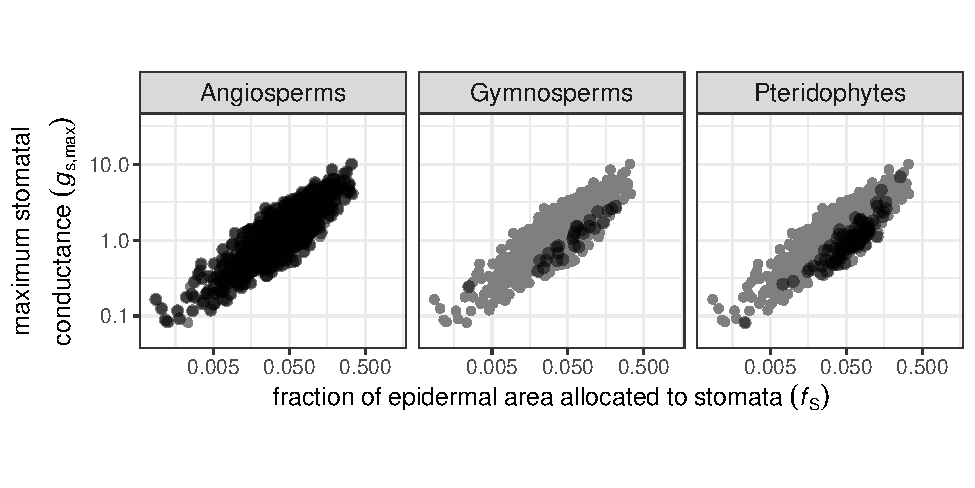
\includegraphics{figures/fig-gmax-fs.pdf}
\end{figure}

\newpage

\begin{figure}
\caption{The effect of mutational variance and strength of selection on $g_\mathrm{s,max}$ on the additive genetic variance within species under $H_2$: stomatal-area minimization hypothesis. The additive genetic variance within species at mutation-selection balance in stomatal density (left panel) and size (right panel) depends on mutational variance ($M_{d_\mathrm{S}}$ and $M_{a_\mathrm{S}}$) and the strength of selection on $g_\mathrm{s,max}$ ($\omega$). In the left panel, $M_{a_\mathrm{S}} = 3.77 \times 10^{-7}$ while $M_{d_\mathrm{S}}$ varied; in the right panel, $M_{d_\mathrm{S}} = 3.77 \times 10^{-7}$ while $M_{a_\mathrm{S}}$ varied. The strength of selection on $g_\mathrm{s,max}$ varied between $\omega = 7.54 \times 10^{-2}$ (weak, solid line), $\omega = 3.77 \times 10^{-2}$ (medium, dotted line), and $\omega = 1.89 \times 10^{-2}$ (strong, dashed line). We also assumed no mutational correlation and $\phi_f = 2$. See text for explanation of parameter values. Note that both stomatal density and size are expressed on a log-scale.}
% Created by tikzDevice version 0.12.6 on 2025-08-19 18:43:05
% !TEX encoding = UTF-8 Unicode
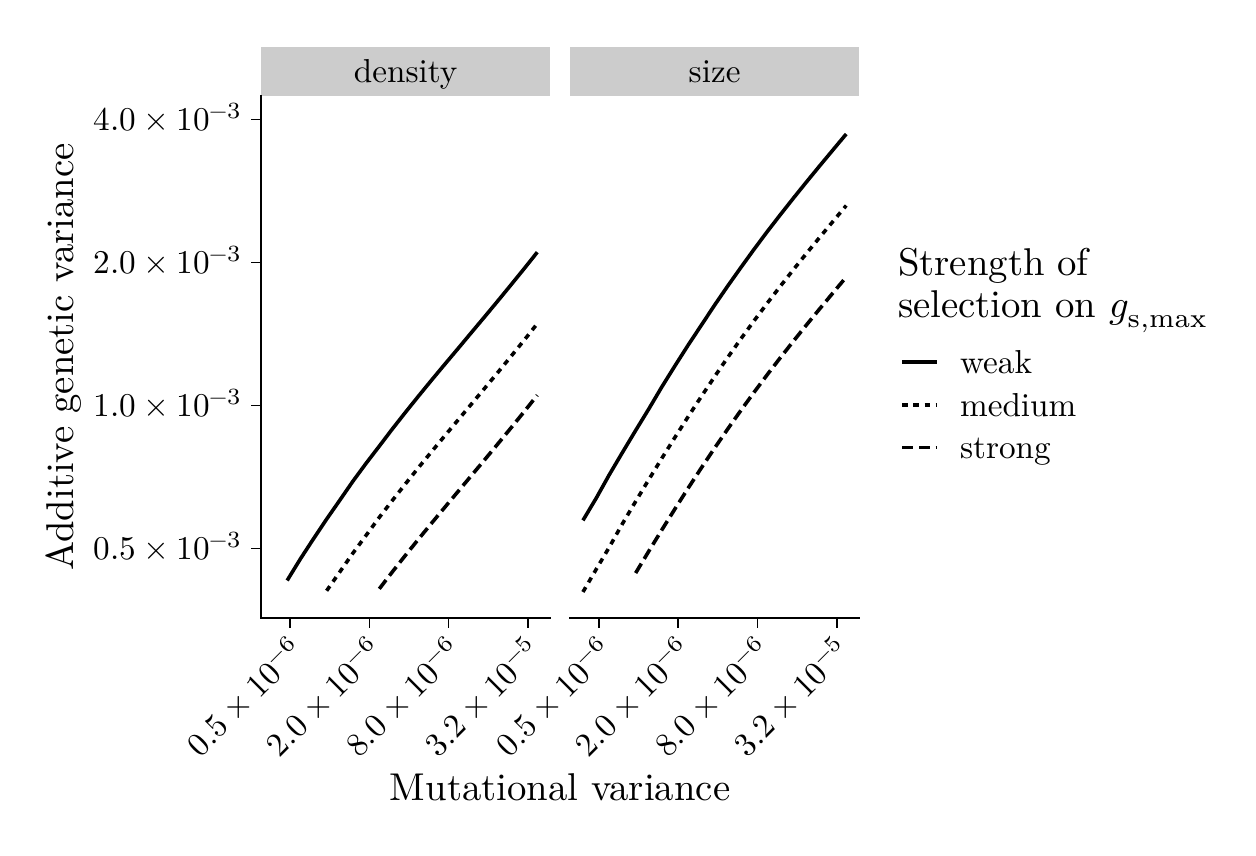
\begin{tikzpicture}[x=1pt,y=1pt]
\definecolor{fillColor}{RGB}{255,255,255}
\path[use as bounding box,fill=fillColor,fill opacity=0.00] (0,0) rectangle (433.62,289.08);
\begin{scope}
\path[clip] ( 84.25, 75.67) rectangle (188.89,264.48);
\definecolor{drawColor}{RGB}{0,0,0}

\path[draw=drawColor,line width= 1.3pt,line join=round] ( 93.76, 89.32) --
	( 98.52, 97.08) --
	(103.27,104.38) --
	(108.03,111.49) --
	(112.79,118.33) --
	(117.54,125.21) --
	(122.30,131.67) --
	(127.06,137.87) --
	(131.81,144.12) --
	(136.57,150.16) --
	(141.33,156.08) --
	(146.08,161.88) --
	(150.84,167.58) --
	(155.60,173.23) --
	(160.35,178.92) --
	(165.11,184.59) --
	(169.87,190.32) --
	(174.62,196.11) --
	(179.38,201.97) --
	(184.14,207.94);

\path[draw=drawColor,line width= 1.3pt,dash pattern=on 2pt off 2pt ,line join=round] (108.03, 85.61) --
	(112.79, 92.42) --
	(117.54, 99.22) --
	(122.30,105.64) --
	(127.06,112.13) --
	(131.81,118.27) --
	(136.57,124.31) --
	(141.33,130.25) --
	(146.08,136.02) --
	(150.84,141.74) --
	(155.60,147.41) --
	(160.35,153.08) --
	(165.11,158.75) --
	(169.87,164.47) --
	(174.62,170.26) --
	(179.38,176.13) --
	(184.14,182.11);

\path[draw=drawColor,line width= 1.3pt,dash pattern=on 4pt off 2pt ,line join=round] (127.06, 86.31) --
	(131.81, 92.48) --
	(136.57, 98.50) --
	(141.33,104.39) --
	(146.08,110.18) --
	(150.84,115.90) --
	(155.60,121.58) --
	(160.35,127.24) --
	(165.11,132.92) --
	(169.87,138.65) --
	(174.62,144.43) --
	(179.38,150.30) --
	(184.14,156.27);
\end{scope}
\begin{scope}
\path[clip] (195.89, 75.67) rectangle (300.54,264.48);
\definecolor{drawColor}{RGB}{0,0,0}

\path[draw=drawColor,line width= 1.3pt,line join=round] (200.65,111.05) --
	(205.41,119.01) --
	(210.16,127.53) --
	(214.92,135.59) --
	(219.68,143.51) --
	(224.43,151.29) --
	(229.19,159.34) --
	(233.95,166.98) --
	(238.70,174.43) --
	(243.46,181.62) --
	(248.22,188.82) --
	(252.97,195.74) --
	(257.73,202.44) --
	(262.49,209.02) --
	(267.24,215.37) --
	(272.00,221.53) --
	(276.76,227.55) --
	(281.51,233.44) --
	(286.27,239.24) --
	(291.03,244.96) --
	(295.78,250.64);

\path[draw=drawColor,line width= 1.3pt,dash pattern=on 2pt off 2pt ,line join=round] (200.65, 85.17) --
	(205.41, 93.32) --
	(210.16,101.35) --
	(214.92,109.84) --
	(219.68,117.87) --
	(224.43,125.76) --
	(229.19,133.53) --
	(233.95,141.13) --
	(238.70,148.58) --
	(243.46,155.86) --
	(248.22,162.99) --
	(252.97,169.93) --
	(257.73,176.65) --
	(262.49,183.17) --
	(267.24,189.52) --
	(272.00,195.69) --
	(276.76,201.72) --
	(281.51,207.62) --
	(286.27,213.41) --
	(291.03,219.12) --
	(295.78,224.80);

\path[draw=drawColor,line width= 1.3pt,dash pattern=on 4pt off 2pt ,line join=round] (219.68, 92.00) --
	(224.43, 99.88) --
	(229.19,107.66) --
	(233.95,115.28) --
	(238.70,122.75) --
	(243.46,130.05) --
	(248.22,137.16) --
	(252.97,144.07) --
	(257.73,150.80) --
	(262.49,157.34) --
	(267.24,163.68) --
	(272.00,169.86) --
	(276.76,175.88) --
	(281.51,181.78) --
	(286.27,187.57) --
	(291.03,193.29) --
	(295.78,198.96);
\end{scope}
\begin{scope}
\path[clip] ( 84.25,264.48) rectangle (188.89,282.08);
\definecolor{fillColor}{gray}{0.80}

\path[fill=fillColor] ( 84.25,264.48) rectangle (188.89,282.08);
\definecolor{drawColor}{RGB}{0,0,0}

\node[text=drawColor,anchor=base,inner sep=0pt, outer sep=0pt, scale=  1.20] at (136.57,269.15) {density};
\end{scope}
\begin{scope}
\path[clip] (195.89,264.48) rectangle (300.54,282.08);
\definecolor{fillColor}{gray}{0.80}

\path[fill=fillColor] (195.89,264.48) rectangle (300.54,282.08);
\definecolor{drawColor}{RGB}{0,0,0}

\node[text=drawColor,anchor=base,inner sep=0pt, outer sep=0pt, scale=  1.20] at (248.22,269.15) {size};
\end{scope}
\begin{scope}
\path[clip] (  0.00,  0.00) rectangle (433.62,289.08);
\definecolor{drawColor}{RGB}{0,0,0}

\path[draw=drawColor,line width= 0.6pt,line join=round,line cap=rect] ( 84.25, 75.67) --
	(188.89, 75.67);
\end{scope}
\begin{scope}
\path[clip] (  0.00,  0.00) rectangle (433.62,289.08);
\definecolor{drawColor}{RGB}{0,0,0}

\path[draw=drawColor,line width= 0.6pt,line join=round] ( 94.82, 72.17) --
	( 94.82, 75.67);

\path[draw=drawColor,line width= 0.6pt,line join=round] (123.46, 72.17) --
	(123.46, 75.67);

\path[draw=drawColor,line width= 0.6pt,line join=round] (152.10, 72.17) --
	(152.10, 75.67);

\path[draw=drawColor,line width= 0.6pt,line join=round] (180.73, 72.17) --
	(180.73, 75.67);
\end{scope}
\begin{scope}
\path[clip] (  0.00,  0.00) rectangle (433.62,289.08);
\definecolor{drawColor}{RGB}{0,0,0}

\node[text=drawColor,rotate= 45.00,anchor=base east,inner sep=0pt, outer sep=0pt, scale=  1.20] at (100.66, 63.32) {$0.5 \times 10^{-6}$};

\node[text=drawColor,rotate= 45.00,anchor=base east,inner sep=0pt, outer sep=0pt, scale=  1.20] at (129.30, 63.32) {$2.0 \times 10^{-6}$};

\node[text=drawColor,rotate= 45.00,anchor=base east,inner sep=0pt, outer sep=0pt, scale=  1.20] at (157.94, 63.32) {$8.0 \times 10^{-6}$};

\node[text=drawColor,rotate= 45.00,anchor=base east,inner sep=0pt, outer sep=0pt, scale=  1.20] at (186.58, 63.32) {$3.2 \times 10^{-5}$};
\end{scope}
\begin{scope}
\path[clip] (  0.00,  0.00) rectangle (433.62,289.08);
\definecolor{drawColor}{RGB}{0,0,0}

\path[draw=drawColor,line width= 0.6pt,line join=round,line cap=rect] (195.89, 75.67) --
	(300.54, 75.67);
\end{scope}
\begin{scope}
\path[clip] (  0.00,  0.00) rectangle (433.62,289.08);
\definecolor{drawColor}{RGB}{0,0,0}

\path[draw=drawColor,line width= 0.6pt,line join=round] (206.47, 72.17) --
	(206.47, 75.67);

\path[draw=drawColor,line width= 0.6pt,line join=round] (235.11, 72.17) --
	(235.11, 75.67);

\path[draw=drawColor,line width= 0.6pt,line join=round] (263.74, 72.17) --
	(263.74, 75.67);

\path[draw=drawColor,line width= 0.6pt,line join=round] (292.38, 72.17) --
	(292.38, 75.67);
\end{scope}
\begin{scope}
\path[clip] (  0.00,  0.00) rectangle (433.62,289.08);
\definecolor{drawColor}{RGB}{0,0,0}

\node[text=drawColor,rotate= 45.00,anchor=base east,inner sep=0pt, outer sep=0pt, scale=  1.20] at (212.31, 63.32) {$0.5 \times 10^{-6}$};

\node[text=drawColor,rotate= 45.00,anchor=base east,inner sep=0pt, outer sep=0pt, scale=  1.20] at (240.95, 63.32) {$2.0 \times 10^{-6}$};

\node[text=drawColor,rotate= 45.00,anchor=base east,inner sep=0pt, outer sep=0pt, scale=  1.20] at (269.59, 63.32) {$8.0 \times 10^{-6}$};

\node[text=drawColor,rotate= 45.00,anchor=base east,inner sep=0pt, outer sep=0pt, scale=  1.20] at (298.23, 63.32) {$3.2 \times 10^{-5}$};
\end{scope}
\begin{scope}
\path[clip] (  0.00,  0.00) rectangle (433.62,289.08);
\definecolor{drawColor}{RGB}{0,0,0}

\path[draw=drawColor,line width= 0.6pt,line join=round,line cap=rect] ( 84.25, 75.67) --
	( 84.25,264.48);
\end{scope}
\begin{scope}
\path[clip] (  0.00,  0.00) rectangle (433.62,289.08);
\definecolor{drawColor}{RGB}{0,0,0}

\node[text=drawColor,anchor=base east,inner sep=0pt, outer sep=0pt, scale=  1.20] at ( 77.75, 96.75) {$0.5 \times 10^{-3}$};

\node[text=drawColor,anchor=base east,inner sep=0pt, outer sep=0pt, scale=  1.20] at ( 77.75,148.42) {$1.0 \times 10^{-3}$};

\node[text=drawColor,anchor=base east,inner sep=0pt, outer sep=0pt, scale=  1.20] at ( 77.75,200.10) {$2.0 \times 10^{-3}$};

\node[text=drawColor,anchor=base east,inner sep=0pt, outer sep=0pt, scale=  1.20] at ( 77.75,251.77) {$4.0 \times 10^{-3}$};
\end{scope}
\begin{scope}
\path[clip] (  0.00,  0.00) rectangle (433.62,289.08);
\definecolor{drawColor}{RGB}{0,0,0}

\path[draw=drawColor,line width= 0.6pt,line join=round] ( 80.75,100.88) --
	( 84.25,100.88);

\path[draw=drawColor,line width= 0.6pt,line join=round] ( 80.75,152.56) --
	( 84.25,152.56);

\path[draw=drawColor,line width= 0.6pt,line join=round] ( 80.75,204.23) --
	( 84.25,204.23);

\path[draw=drawColor,line width= 0.6pt,line join=round] ( 80.75,255.90) --
	( 84.25,255.90);
\end{scope}
\begin{scope}
\path[clip] (  0.00,  0.00) rectangle (433.62,289.08);
\definecolor{drawColor}{RGB}{0,0,0}

\node[text=drawColor,anchor=base,inner sep=0pt, outer sep=0pt, scale=  1.40] at (192.39,  9.72) {Mutational variance};
\end{scope}
\begin{scope}
\path[clip] (  0.00,  0.00) rectangle (433.62,289.08);
\definecolor{drawColor}{RGB}{0,0,0}

\node[text=drawColor,rotate= 90.00,anchor=base,inner sep=0pt, outer sep=0pt, scale=  1.40] at ( 16.64,170.07) {Additive genetic variance};
\end{scope}
\begin{scope}
\path[clip] (  0.00,  0.00) rectangle (433.62,289.08);
\definecolor{drawColor}{RGB}{0,0,0}

\node[text=drawColor,anchor=base west,inner sep=0pt, outer sep=0pt, scale=  1.40] at (314.54,199.41) {Strength of};

\node[text=drawColor,anchor=base west,inner sep=0pt, outer sep=0pt, scale=  1.40] at (314.54,184.29) {selection on $g_\mathrm{s,max}$};
\end{scope}
\begin{scope}
\path[clip] (  0.00,  0.00) rectangle (433.62,289.08);
\definecolor{drawColor}{RGB}{0,0,0}

\path[draw=drawColor,line width= 1.3pt,line join=round] (316.08,168.23) -- (328.40,168.23);
\end{scope}
\begin{scope}
\path[clip] (  0.00,  0.00) rectangle (433.62,289.08);
\definecolor{drawColor}{RGB}{0,0,0}

\path[draw=drawColor,line width= 1.3pt,dash pattern=on 2pt off 2pt ,line join=round] (316.08,152.83) -- (328.40,152.83);
\end{scope}
\begin{scope}
\path[clip] (  0.00,  0.00) rectangle (433.62,289.08);
\definecolor{drawColor}{RGB}{0,0,0}

\path[draw=drawColor,line width= 1.3pt,dash pattern=on 4pt off 2pt ,line join=round] (316.08,137.43) -- (328.40,137.43);
\end{scope}
\begin{scope}
\path[clip] (  0.00,  0.00) rectangle (433.62,289.08);
\definecolor{drawColor}{RGB}{0,0,0}

\node[text=drawColor,anchor=base west,inner sep=0pt, outer sep=0pt, scale=  1.20] at (336.94,164.10) {weak};
\end{scope}
\begin{scope}
\path[clip] (  0.00,  0.00) rectangle (433.62,289.08);
\definecolor{drawColor}{RGB}{0,0,0}

\node[text=drawColor,anchor=base west,inner sep=0pt, outer sep=0pt, scale=  1.20] at (336.94,148.70) {medium};
\end{scope}
\begin{scope}
\path[clip] (  0.00,  0.00) rectangle (433.62,289.08);
\definecolor{drawColor}{RGB}{0,0,0}

\node[text=drawColor,anchor=base west,inner sep=0pt, outer sep=0pt, scale=  1.20] at (336.94,133.30) {strong};
\end{scope}
\end{tikzpicture}

\end{figure}

\newpage

\begin{figure}
\caption{The effect of mutational correlation between stomtal density and size ($\rho_\mathrm{M}$) on the additive genetic correlation under $H_2$: stomatal-area minimization hypothesis. The additive genetic correlation between stomatal density and size within species at mutation-selection balance depends on mutational correlation and the strength of selection on $f_\mathrm{S}$ ($\phi_f$). The strength of selection on stomatal size varied between $\phi_f = 0.5$ (strong, solid line), $\phi_f = 1$ (medium, dotted line), and $\phi_f = 2$ (weak, dashed line). Other parameters were set to $M_{d_\mathrm{S}} = M_{a_\mathrm{S}} = 3.77 \times 10^{-7}$ and $\omega = 3.77 \times 10^{-2}$. See text for explanation of parameter values.}
% Created by tikzDevice version 0.12.6 on 2025-08-19 18:43:19
% !TEX encoding = UTF-8 Unicode
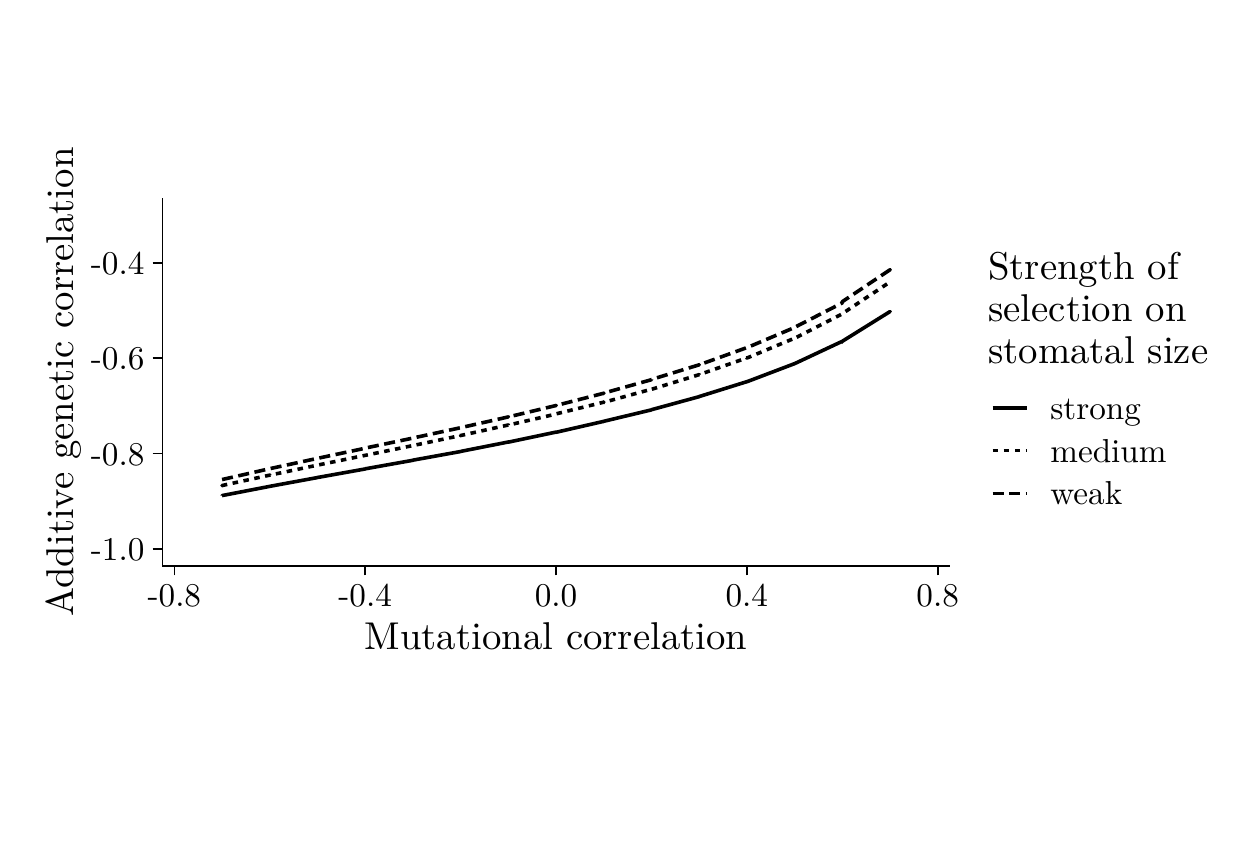
\begin{tikzpicture}[x=1pt,y=1pt]
\definecolor{fillColor}{RGB}{255,255,255}
\path[use as bounding box,fill=fillColor,fill opacity=0.00] (0,0) rectangle (433.62,289.08);
\begin{scope}
\path[clip] ( 48.69, 94.65) rectangle (333.15,227.39);
\definecolor{drawColor}{RGB}{0,0,0}

\path[draw=drawColor,line width= 1.3pt,line join=round] ( 70.24,119.98) --
	( 70.24,120.00) --
	( 87.48,123.33) --
	( 87.48,123.34) --
	(104.72,126.51) --
	(104.72,126.53) --
	(121.96,129.62) --
	(121.96,129.67) --
	(139.20,132.75) --
	(139.20,132.79) --
	(139.20,132.80) --
	(156.44,135.92) --
	(156.44,136.00) --
	(156.44,135.96) --
	(173.68,139.36) --
	(173.68,139.37) --
	(173.68,139.31) --
	(190.92,142.94) --
	(190.92,142.94) --
	(190.92,142.87) --
	(208.16,146.82) --
	(208.16,146.74) --
	(208.16,146.84) --
	(225.40,150.97) --
	(225.40,150.97) --
	(225.40,151.03) --
	(242.64,155.74) --
	(242.64,155.72) --
	(242.64,155.78) --
	(259.88,161.16) --
	(259.88,161.16) --
	(259.88,161.13) --
	(277.12,167.68) --
	(277.12,167.57) --
	(277.12,167.67) --
	(294.36,175.75) --
	(294.36,175.46) --
	(294.36,175.75) --
	(311.60,186.49) --
	(311.60,186.44) --
	(311.60,186.45);

\path[draw=drawColor,line width= 1.3pt,dash pattern=on 2pt off 2pt ,line join=round] ( 70.24,123.58) --
	( 70.24,123.56) --
	( 70.24,123.63) --
	( 87.48,127.39) --
	( 87.48,127.37) --
	( 87.48,127.37) --
	(104.72,131.00) --
	(104.72,131.00) --
	(104.72,131.00) --
	(121.96,134.54) --
	(121.96,134.55) --
	(121.96,134.53) --
	(139.20,138.08) --
	(139.20,138.11) --
	(139.20,138.07) --
	(156.44,141.70) --
	(156.44,141.72) --
	(156.44,141.70) --
	(173.68,145.51) --
	(173.68,145.49) --
	(173.68,145.47) --
	(190.92,149.45) --
	(190.92,149.46) --
	(190.92,149.52) --
	(208.16,153.74) --
	(208.16,153.83) --
	(208.16,153.69) --
	(225.40,158.44) --
	(225.40,158.52) --
	(225.40,158.39) --
	(242.64,163.70) --
	(242.64,163.70) --
	(242.64,163.69) --
	(259.88,169.76) --
	(259.88,169.74) --
	(259.88,169.69) --
	(277.12,176.87) --
	(277.12,176.94) --
	(277.12,176.81) --
	(294.36,185.67) --
	(294.36,185.68) --
	(294.36,185.74) --
	(311.60,197.19) --
	(311.60,197.16) --
	(311.60,197.23);

\path[draw=drawColor,line width= 1.3pt,dash pattern=on 4pt off 2pt ,line join=round] ( 70.24,125.79) --
	( 70.24,125.79) --
	( 87.48,129.72) --
	( 87.48,129.72) --
	(104.72,133.45) --
	(104.72,133.45) --
	(121.96,137.11) --
	(121.96,137.16) --
	(139.20,140.77) --
	(139.20,140.79) --
	(139.20,140.80) --
	(156.44,144.52) --
	(156.44,144.52) --
	(156.44,144.53) --
	(173.68,148.42) --
	(173.68,148.38) --
	(173.68,148.42) --
	(190.92,152.54) --
	(190.92,152.48) --
	(190.92,152.55) --
	(208.16,156.98) --
	(208.16,156.89) --
	(208.16,157.03) --
	(225.40,161.87) --
	(225.40,161.87) --
	(225.40,161.95) --
	(242.64,167.25) --
	(242.64,167.29) --
	(242.64,167.24) --
	(259.88,173.47) --
	(259.88,173.47) --
	(259.88,173.43) --
	(277.12,180.74) --
	(277.12,180.85) --
	(277.12,180.78) --
	(294.36,189.63) --
	(294.36,189.83) --
	(294.36,190.06) --
	(311.60,201.60) --
	(311.60,201.53) --
	(311.60,201.72);
\end{scope}
\begin{scope}
\path[clip] (  0.00,  0.00) rectangle (433.62,289.08);
\definecolor{drawColor}{RGB}{0,0,0}

\path[draw=drawColor,line width= 0.6pt,line join=round,line cap=rect] ( 48.69, 94.65) --
	( 48.69,227.39);
\end{scope}
\begin{scope}
\path[clip] (  0.00,  0.00) rectangle (433.62,289.08);
\definecolor{drawColor}{RGB}{0,0,0}

\node[text=drawColor,anchor=base east,inner sep=0pt, outer sep=0pt, scale=  1.20] at ( 42.19, 96.55) {-1.0};

\node[text=drawColor,anchor=base east,inner sep=0pt, outer sep=0pt, scale=  1.20] at ( 42.19,131.03) {-0.8};

\node[text=drawColor,anchor=base east,inner sep=0pt, outer sep=0pt, scale=  1.20] at ( 42.19,165.51) {-0.6};

\node[text=drawColor,anchor=base east,inner sep=0pt, outer sep=0pt, scale=  1.20] at ( 42.19,199.99) {-0.4};
\end{scope}
\begin{scope}
\path[clip] (  0.00,  0.00) rectangle (433.62,289.08);
\definecolor{drawColor}{RGB}{0,0,0}

\path[draw=drawColor,line width= 0.6pt,line join=round] ( 45.19,100.68) --
	( 48.69,100.68);

\path[draw=drawColor,line width= 0.6pt,line join=round] ( 45.19,135.16) --
	( 48.69,135.16);

\path[draw=drawColor,line width= 0.6pt,line join=round] ( 45.19,169.64) --
	( 48.69,169.64);

\path[draw=drawColor,line width= 0.6pt,line join=round] ( 45.19,204.12) --
	( 48.69,204.12);
\end{scope}
\begin{scope}
\path[clip] (  0.00,  0.00) rectangle (433.62,289.08);
\definecolor{drawColor}{RGB}{0,0,0}

\path[draw=drawColor,line width= 0.6pt,line join=round,line cap=rect] ( 48.69, 94.65) --
	(333.15, 94.65);
\end{scope}
\begin{scope}
\path[clip] (  0.00,  0.00) rectangle (433.62,289.08);
\definecolor{drawColor}{RGB}{0,0,0}

\path[draw=drawColor,line width= 0.6pt,line join=round] ( 53.00, 91.15) --
	( 53.00, 94.65);

\path[draw=drawColor,line width= 0.6pt,line join=round] (121.96, 91.15) --
	(121.96, 94.65);

\path[draw=drawColor,line width= 0.6pt,line join=round] (190.92, 91.15) --
	(190.92, 94.65);

\path[draw=drawColor,line width= 0.6pt,line join=round] (259.88, 91.15) --
	(259.88, 94.65);

\path[draw=drawColor,line width= 0.6pt,line join=round] (328.84, 91.15) --
	(328.84, 94.65);
\end{scope}
\begin{scope}
\path[clip] (  0.00,  0.00) rectangle (433.62,289.08);
\definecolor{drawColor}{RGB}{0,0,0}

\node[text=drawColor,anchor=base,inner sep=0pt, outer sep=0pt, scale=  1.20] at ( 53.00, 79.88) {-0.8};

\node[text=drawColor,anchor=base,inner sep=0pt, outer sep=0pt, scale=  1.20] at (121.96, 79.88) {-0.4};

\node[text=drawColor,anchor=base,inner sep=0pt, outer sep=0pt, scale=  1.20] at (190.92, 79.88) {0.0};

\node[text=drawColor,anchor=base,inner sep=0pt, outer sep=0pt, scale=  1.20] at (259.88, 79.88) {0.4};

\node[text=drawColor,anchor=base,inner sep=0pt, outer sep=0pt, scale=  1.20] at (328.84, 79.88) {0.8};
\end{scope}
\begin{scope}
\path[clip] (  0.00,  0.00) rectangle (433.62,289.08);
\definecolor{drawColor}{RGB}{0,0,0}

\node[text=drawColor,anchor=base,inner sep=0pt, outer sep=0pt, scale=  1.40] at (190.92, 64.41) {Mutational correlation};
\end{scope}
\begin{scope}
\path[clip] (  0.00,  0.00) rectangle (433.62,289.08);
\definecolor{drawColor}{RGB}{0,0,0}

\node[text=drawColor,rotate= 90.00,anchor=base,inner sep=0pt, outer sep=0pt, scale=  1.40] at ( 16.64,161.02) {Additive genetic correlation};
\end{scope}
\begin{scope}
\path[clip] (  0.00,  0.00) rectangle (433.62,289.08);
\definecolor{drawColor}{RGB}{0,0,0}

\node[text=drawColor,anchor=base west,inner sep=0pt, outer sep=0pt, scale=  1.40] at (347.15,197.92) {Strength of};

\node[text=drawColor,anchor=base west,inner sep=0pt, outer sep=0pt, scale=  1.40] at (347.15,182.80) {selection on};

\node[text=drawColor,anchor=base west,inner sep=0pt, outer sep=0pt, scale=  1.40] at (347.15,167.68) {stomatal size};
\end{scope}
\begin{scope}
\path[clip] (  0.00,  0.00) rectangle (433.62,289.08);
\definecolor{drawColor}{RGB}{0,0,0}

\path[draw=drawColor,line width= 1.3pt,line join=round] (348.69,151.62) -- (361.01,151.62);
\end{scope}
\begin{scope}
\path[clip] (  0.00,  0.00) rectangle (433.62,289.08);
\definecolor{drawColor}{RGB}{0,0,0}

\path[draw=drawColor,line width= 1.3pt,dash pattern=on 2pt off 2pt ,line join=round] (348.69,136.22) -- (361.01,136.22);
\end{scope}
\begin{scope}
\path[clip] (  0.00,  0.00) rectangle (433.62,289.08);
\definecolor{drawColor}{RGB}{0,0,0}

\path[draw=drawColor,line width= 1.3pt,dash pattern=on 4pt off 2pt ,line join=round] (348.69,120.82) -- (361.01,120.82);
\end{scope}
\begin{scope}
\path[clip] (  0.00,  0.00) rectangle (433.62,289.08);
\definecolor{drawColor}{RGB}{0,0,0}

\node[text=drawColor,anchor=base west,inner sep=0pt, outer sep=0pt, scale=  1.20] at (369.55,147.49) {strong};
\end{scope}
\begin{scope}
\path[clip] (  0.00,  0.00) rectangle (433.62,289.08);
\definecolor{drawColor}{RGB}{0,0,0}

\node[text=drawColor,anchor=base west,inner sep=0pt, outer sep=0pt, scale=  1.20] at (369.55,132.09) {medium};
\end{scope}
\begin{scope}
\path[clip] (  0.00,  0.00) rectangle (433.62,289.08);
\definecolor{drawColor}{RGB}{0,0,0}

\node[text=drawColor,anchor=base west,inner sep=0pt, outer sep=0pt, scale=  1.20] at (369.55,116.69) {weak};
\end{scope}
\end{tikzpicture}

\end{figure}

\newpage

\begin{figure}
\caption{The effect of selection on and mutational variance in stomatal size on the additive genetic variance under $H_2$: stomatal-area minimization hypothesis. The ratio of additive genetic variance within species at mutation-selection balance in stomatal density and size depends on the relative mutational variance ($M_{d_\mathrm{S}} / M_{a_\mathrm{S}}$) and the strength of selection on $f_\mathrm{S}$ ($\phi_f \omega$). Results are shown for $M_{d_\mathrm{S}} = 3.77 \times 10^{-7}$ while $M_{a_\mathrm{S}}$ varied from $0.1 M_{d_\mathrm{S}}$ (low, solid line), $M_{d_\mathrm{S}}$ (medium, dotted line), and $10 M_{d_\mathrm{S}}$ (high, dashed line). The relative strength of selection on $f_\mathrm{S}$ varied between $\phi_f = 0.5$ and 2. We also assumed no mutational correlation and $\omega = 3.77 \times 10^{-2}$. See text for explanation of parameter values.}
% Created by tikzDevice version 0.12.6 on 2025-08-19 18:43:27
% !TEX encoding = UTF-8 Unicode
\begin{tikzpicture}[x=1pt,y=1pt]
\definecolor{fillColor}{RGB}{255,255,255}
\path[use as bounding box,fill=fillColor,fill opacity=0.00] (0,0) rectangle (433.62,289.08);
\begin{scope}
\path[clip] (118.07, 39.96) rectangle (222.34,282.08);
\definecolor{drawColor}{RGB}{0,0,0}

\path[draw=drawColor,line width= 1.3pt,line join=round] (122.81,183.61) --
	(134.66,183.04) --
	(146.51,182.17) --
	(158.36,181.01) --
	(170.21,179.79) --
	(182.06,178.04) --
	(193.91,176.01) --
	(205.76,173.71) --
	(217.60,171.17);

\path[draw=drawColor,line width= 1.3pt,dash pattern=on 2pt off 2pt ,line join=round] (122.81,145.57) --
	(134.66,143.58) --
	(146.51,141.43) --
	(158.36,139.11) --
	(170.21,136.63) --
	(182.06,134.03) --
	(193.91,131.31) --
	(205.76,128.45) --
	(217.60,125.54);

\path[draw=drawColor,line width= 1.3pt,dash pattern=on 4pt off 2pt ,line join=round] (122.81,109.74) --
	(134.66,106.65) --
	(146.51,103.52) --
	(158.36,100.35) --
	(170.21, 97.19) --
	(182.06, 94.05) --
	(193.91, 90.96) --
	(205.76, 87.95) --
	(217.60, 85.04);
\end{scope}
\begin{scope}
\path[clip] (  0.00,  0.00) rectangle (433.62,289.08);
\definecolor{drawColor}{RGB}{0,0,0}

\path[draw=drawColor,line width= 0.6pt,line join=round,line cap=rect] (118.07, 39.96) --
	(118.07,282.08);
\end{scope}
\begin{scope}
\path[clip] (  0.00,  0.00) rectangle (433.62,289.08);
\definecolor{drawColor}{RGB}{0,0,0}

\node[text=drawColor,anchor=base east,inner sep=0pt, outer sep=0pt, scale=  1.20] at (111.57, 62.09) {0.25};

\node[text=drawColor,anchor=base east,inner sep=0pt, outer sep=0pt, scale=  1.20] at (111.57,156.89) {1.00};

\node[text=drawColor,anchor=base east,inner sep=0pt, outer sep=0pt, scale=  1.20] at (111.57,251.68) {4.00};
\end{scope}
\begin{scope}
\path[clip] (  0.00,  0.00) rectangle (433.62,289.08);
\definecolor{drawColor}{RGB}{0,0,0}

\path[draw=drawColor,line width= 0.6pt,line join=round] (114.57, 66.23) --
	(118.07, 66.23);

\path[draw=drawColor,line width= 0.6pt,line join=round] (114.57,161.02) --
	(118.07,161.02);

\path[draw=drawColor,line width= 0.6pt,line join=round] (114.57,255.82) --
	(118.07,255.82);
\end{scope}
\begin{scope}
\path[clip] (  0.00,  0.00) rectangle (433.62,289.08);
\definecolor{drawColor}{RGB}{0,0,0}

\path[draw=drawColor,line width= 0.6pt,line join=round,line cap=rect] (118.07, 39.96) --
	(222.34, 39.96);
\end{scope}
\begin{scope}
\path[clip] (  0.00,  0.00) rectangle (433.62,289.08);
\definecolor{drawColor}{RGB}{0,0,0}

\path[draw=drawColor,line width= 0.6pt,line join=round] (122.81, 36.46) --
	(122.81, 39.96);

\path[draw=drawColor,line width= 0.6pt,line join=round] (170.21, 36.46) --
	(170.21, 39.96);

\path[draw=drawColor,line width= 0.6pt,line join=round] (217.60, 36.46) --
	(217.60, 39.96);
\end{scope}
\begin{scope}
\path[clip] (  0.00,  0.00) rectangle (433.62,289.08);
\definecolor{drawColor}{RGB}{0,0,0}

\node[text=drawColor,anchor=base,inner sep=0pt, outer sep=0pt, scale=  1.20] at (122.81, 25.20) {$0.5\omega$};

\node[text=drawColor,anchor=base,inner sep=0pt, outer sep=0pt, scale=  1.20] at (170.21, 25.20) {$1\omega$};

\node[text=drawColor,anchor=base,inner sep=0pt, outer sep=0pt, scale=  1.20] at (217.60, 25.20) {$2\omega$};
\end{scope}
\begin{scope}
\path[clip] (  0.00,  0.00) rectangle (433.62,289.08);
\definecolor{drawColor}{RGB}{0,0,0}

\node[text=drawColor,anchor=base,inner sep=0pt, outer sep=0pt, scale=  1.40] at (170.21,  9.72) {Strength of selection on $f_\mathrm{S}$};
\end{scope}
\begin{scope}
\path[clip] (  0.00,  0.00) rectangle (433.62,289.08);
\definecolor{drawColor}{RGB}{0,0,0}

\node[text=drawColor,rotate= 90.00,anchor=base,inner sep=0pt, outer sep=0pt, scale=  1.40] at ( 84.02,161.02) {Relative genetic variance, $G^*_{d_\mathrm{S}} / G^*_{a_\mathrm{S}}$};
\end{scope}
\begin{scope}
\path[clip] (  0.00,  0.00) rectangle (433.62,289.08);
\definecolor{drawColor}{RGB}{0,0,0}

\node[text=drawColor,anchor=base west,inner sep=0pt, outer sep=0pt, scale=  1.40] at (236.34,190.36) {Mutational variance};

\node[text=drawColor,anchor=base west,inner sep=0pt, outer sep=0pt, scale=  1.40] at (236.34,175.24) {of stomatal size};
\end{scope}
\begin{scope}
\path[clip] (  0.00,  0.00) rectangle (433.62,289.08);
\definecolor{drawColor}{RGB}{0,0,0}

\path[draw=drawColor,line width= 1.3pt,line join=round] (237.88,159.18) -- (250.20,159.18);
\end{scope}
\begin{scope}
\path[clip] (  0.00,  0.00) rectangle (433.62,289.08);
\definecolor{drawColor}{RGB}{0,0,0}

\path[draw=drawColor,line width= 1.3pt,dash pattern=on 2pt off 2pt ,line join=round] (237.88,143.78) -- (250.20,143.78);
\end{scope}
\begin{scope}
\path[clip] (  0.00,  0.00) rectangle (433.62,289.08);
\definecolor{drawColor}{RGB}{0,0,0}

\path[draw=drawColor,line width= 1.3pt,dash pattern=on 4pt off 2pt ,line join=round] (237.88,128.38) -- (250.20,128.38);
\end{scope}
\begin{scope}
\path[clip] (  0.00,  0.00) rectangle (433.62,289.08);
\definecolor{drawColor}{RGB}{0,0,0}

\node[text=drawColor,anchor=base west,inner sep=0pt, outer sep=0pt, scale=  1.20] at (258.74,155.05) {low};
\end{scope}
\begin{scope}
\path[clip] (  0.00,  0.00) rectangle (433.62,289.08);
\definecolor{drawColor}{RGB}{0,0,0}

\node[text=drawColor,anchor=base west,inner sep=0pt, outer sep=0pt, scale=  1.20] at (258.74,139.65) {medium};
\end{scope}
\begin{scope}
\path[clip] (  0.00,  0.00) rectangle (433.62,289.08);
\definecolor{drawColor}{RGB}{0,0,0}

\node[text=drawColor,anchor=base west,inner sep=0pt, outer sep=0pt, scale=  1.20] at (258.74,124.25) {high};
\end{scope}
\end{tikzpicture}

\end{figure}

\newpage

\begin{figure}
\caption{The effect of mutational variance and strength of selection on $g_\mathrm{s,max}$ on the additive genetic variance within species under $H_3$: stomatal adaptation + bounded size hypothesis. The additive genetic variance within species at mutation-selection balance in stomatal density (left panel) and size (right panel) depends on mutational variance ($M_{d_\mathrm{S}}$ and $M_{a_\mathrm{S}}$) and the strength of selection on $g_\mathrm{s,max}$ ($\omega$). In the left panel, $M_{a_\mathrm{S}} = 3.77 \times 10^{-7}$ while $M_{d_\mathrm{S}}$ varied; in the right panel, $M_{d_\mathrm{S}} = 3.77 \times 10^{-7}$ while $M_{a_\mathrm{S}}$ varied. The strength of selection on $g_\mathrm{s,max}$ varied between $\omega = 7.54 \times 10^{-2}$ (weak, solid line), $\omega = 3.77 \times 10^{-2}$ (medium, dotted line), and $\omega = 1.89 \times 10^{-2}$ (strong, dashed line). We also assumed no mutational correlation and $\phi_a = 2$. See text for explanation of parameter values. Note that both stomatal density and size are expressed on a log-scale.}
% Created by tikzDevice version 0.12.6 on 2025-08-19 18:47:20
% !TEX encoding = UTF-8 Unicode
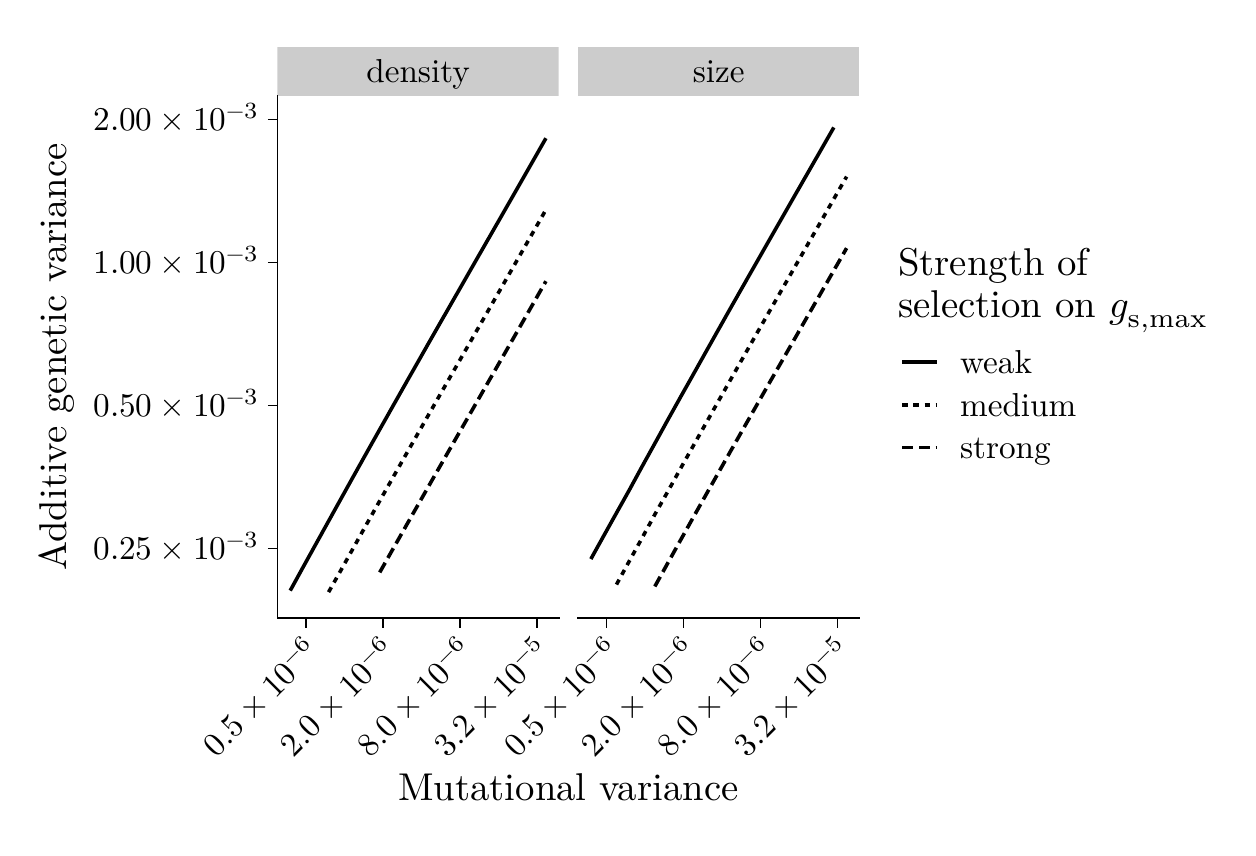
\begin{tikzpicture}[x=1pt,y=1pt]
\definecolor{fillColor}{RGB}{255,255,255}
\path[use as bounding box,fill=fillColor,fill opacity=0.00] (0,0) rectangle (433.62,289.08);
\begin{scope}
\path[clip] ( 90.25, 75.67) rectangle (191.89,264.48);
\definecolor{drawColor}{RGB}{0,0,0}

\path[draw=drawColor,line width= 1.3pt,line join=round] ( 94.87, 85.66) --
	( 99.49, 94.08) --
	(104.11,102.43) --
	(108.73,110.77) --
	(113.35,119.10) --
	(117.97,127.41) --
	(122.59,135.68) --
	(127.21,143.89) --
	(131.83,152.08) --
	(136.45,160.25) --
	(141.07,168.37) --
	(145.69,176.51) --
	(150.31,184.58) --
	(154.93,192.64) --
	(159.55,200.71) --
	(164.17,208.76) --
	(168.79,216.81) --
	(173.41,224.87) --
	(178.03,232.93) --
	(182.65,241.03) --
	(187.27,249.13);

\path[draw=drawColor,line width= 1.3pt,dash pattern=on 2pt off 2pt ,line join=round] (108.73, 85.11) --
	(113.35, 93.31) --
	(117.97,101.59) --
	(122.59,109.88) --
	(127.21,118.08) --
	(131.83,126.25) --
	(136.45,134.40) --
	(141.07,142.53) --
	(145.69,150.65) --
	(150.31,158.73) --
	(154.93,166.80) --
	(159.55,174.86) --
	(164.17,182.92) --
	(168.79,190.98) --
	(173.41,199.03) --
	(178.03,207.11) --
	(182.65,215.19) --
	(187.27,223.29);

\path[draw=drawColor,line width= 1.3pt,dash pattern=on 4pt off 2pt ,line join=round] (127.21, 92.24) --
	(131.83,100.42) --
	(136.45,108.56) --
	(141.07,116.69) --
	(145.69,124.80) --
	(150.31,132.90) --
	(154.93,140.99) --
	(159.55,149.02) --
	(164.17,157.08) --
	(168.79,165.15) --
	(173.41,173.20) --
	(178.03,181.27) --
	(182.65,189.36) --
	(187.27,197.46);
\end{scope}
\begin{scope}
\path[clip] (198.89, 75.67) rectangle (300.54,264.48);
\definecolor{drawColor}{RGB}{0,0,0}

\path[draw=drawColor,line width= 1.3pt,line join=round] (203.51, 97.07) --
	(208.13,105.41) --
	(212.76,113.72) --
	(217.38,121.97) --
	(222.00,130.48) --
	(226.62,138.83) --
	(231.24,147.23) --
	(235.86,155.51) --
	(240.48,163.72) --
	(245.10,171.97) --
	(249.72,180.18) --
	(254.34,188.38) --
	(258.96,196.50) --
	(263.58,204.61) --
	(268.20,212.70) --
	(272.82,220.78) --
	(277.44,228.85) --
	(282.06,236.90) --
	(286.68,244.96) --
	(291.30,253.02);

\path[draw=drawColor,line width= 1.3pt,dash pattern=on 2pt off 2pt ,line join=round] (212.76, 87.86) --
	(217.38, 96.30) --
	(222.00,104.65) --
	(226.62,113.17) --
	(231.24,121.34) --
	(235.86,129.68) --
	(240.48,137.92) --
	(245.10,146.14) --
	(249.72,154.34) --
	(254.34,162.51) --
	(258.96,170.67) --
	(263.58,178.80) --
	(268.20,186.86) --
	(272.82,194.94) --
	(277.44,203.01) --
	(282.06,211.08) --
	(286.68,219.12) --
	(291.30,227.19) --
	(295.92,235.25);

\path[draw=drawColor,line width= 1.3pt,dash pattern=on 4pt off 2pt ,line join=round] (226.62, 87.17) --
	(231.24, 95.50) --
	(235.86,103.80) --
	(240.48,112.08) --
	(245.10,120.29) --
	(249.72,128.49) --
	(254.34,136.67) --
	(258.96,144.81) --
	(263.58,152.94) --
	(268.20,161.05) --
	(272.82,169.10) --
	(277.44,177.17) --
	(282.06,185.24) --
	(286.68,193.28) --
	(291.30,201.34) --
	(295.92,209.41);
\end{scope}
\begin{scope}
\path[clip] ( 90.25,264.48) rectangle (191.89,282.08);
\definecolor{fillColor}{gray}{0.80}

\path[fill=fillColor] ( 90.25,264.48) rectangle (191.89,282.08);
\definecolor{drawColor}{RGB}{0,0,0}

\node[text=drawColor,anchor=base,inner sep=0pt, outer sep=0pt, scale=  1.20] at (141.07,269.15) {density};
\end{scope}
\begin{scope}
\path[clip] (198.89,264.48) rectangle (300.54,282.08);
\definecolor{fillColor}{gray}{0.80}

\path[fill=fillColor] (198.89,264.48) rectangle (300.54,282.08);
\definecolor{drawColor}{RGB}{0,0,0}

\node[text=drawColor,anchor=base,inner sep=0pt, outer sep=0pt, scale=  1.20] at (249.72,269.15) {size};
\end{scope}
\begin{scope}
\path[clip] (  0.00,  0.00) rectangle (433.62,289.08);
\definecolor{drawColor}{RGB}{0,0,0}

\path[draw=drawColor,line width= 0.6pt,line join=round,line cap=rect] ( 90.25, 75.67) --
	(191.89, 75.67);
\end{scope}
\begin{scope}
\path[clip] (  0.00,  0.00) rectangle (433.62,289.08);
\definecolor{drawColor}{RGB}{0,0,0}

\path[draw=drawColor,line width= 0.6pt,line join=round] (100.52, 72.17) --
	(100.52, 75.67);

\path[draw=drawColor,line width= 0.6pt,line join=round] (128.33, 72.17) --
	(128.33, 75.67);

\path[draw=drawColor,line width= 0.6pt,line join=round] (156.15, 72.17) --
	(156.15, 75.67);

\path[draw=drawColor,line width= 0.6pt,line join=round] (183.97, 72.17) --
	(183.97, 75.67);
\end{scope}
\begin{scope}
\path[clip] (  0.00,  0.00) rectangle (433.62,289.08);
\definecolor{drawColor}{RGB}{0,0,0}

\node[text=drawColor,rotate= 45.00,anchor=base east,inner sep=0pt, outer sep=0pt, scale=  1.20] at (106.36, 63.32) {$0.5 \times 10^{-6}$};

\node[text=drawColor,rotate= 45.00,anchor=base east,inner sep=0pt, outer sep=0pt, scale=  1.20] at (134.18, 63.32) {$2.0 \times 10^{-6}$};

\node[text=drawColor,rotate= 45.00,anchor=base east,inner sep=0pt, outer sep=0pt, scale=  1.20] at (162.00, 63.32) {$8.0 \times 10^{-6}$};

\node[text=drawColor,rotate= 45.00,anchor=base east,inner sep=0pt, outer sep=0pt, scale=  1.20] at (189.81, 63.32) {$3.2 \times 10^{-5}$};
\end{scope}
\begin{scope}
\path[clip] (  0.00,  0.00) rectangle (433.62,289.08);
\definecolor{drawColor}{RGB}{0,0,0}

\path[draw=drawColor,line width= 0.6pt,line join=round,line cap=rect] (198.89, 75.67) --
	(300.54, 75.67);
\end{scope}
\begin{scope}
\path[clip] (  0.00,  0.00) rectangle (433.62,289.08);
\definecolor{drawColor}{RGB}{0,0,0}

\path[draw=drawColor,line width= 0.6pt,line join=round] (209.16, 72.17) --
	(209.16, 75.67);

\path[draw=drawColor,line width= 0.6pt,line join=round] (236.98, 72.17) --
	(236.98, 75.67);

\path[draw=drawColor,line width= 0.6pt,line join=round] (264.80, 72.17) --
	(264.80, 75.67);

\path[draw=drawColor,line width= 0.6pt,line join=round] (292.62, 72.17) --
	(292.62, 75.67);
\end{scope}
\begin{scope}
\path[clip] (  0.00,  0.00) rectangle (433.62,289.08);
\definecolor{drawColor}{RGB}{0,0,0}

\node[text=drawColor,rotate= 45.00,anchor=base east,inner sep=0pt, outer sep=0pt, scale=  1.20] at (215.01, 63.32) {$0.5 \times 10^{-6}$};

\node[text=drawColor,rotate= 45.00,anchor=base east,inner sep=0pt, outer sep=0pt, scale=  1.20] at (242.83, 63.32) {$2.0 \times 10^{-6}$};

\node[text=drawColor,rotate= 45.00,anchor=base east,inner sep=0pt, outer sep=0pt, scale=  1.20] at (270.64, 63.32) {$8.0 \times 10^{-6}$};

\node[text=drawColor,rotate= 45.00,anchor=base east,inner sep=0pt, outer sep=0pt, scale=  1.20] at (298.46, 63.32) {$3.2 \times 10^{-5}$};
\end{scope}
\begin{scope}
\path[clip] (  0.00,  0.00) rectangle (433.62,289.08);
\definecolor{drawColor}{RGB}{0,0,0}

\path[draw=drawColor,line width= 0.6pt,line join=round,line cap=rect] ( 90.25, 75.67) --
	( 90.25,264.48);
\end{scope}
\begin{scope}
\path[clip] (  0.00,  0.00) rectangle (433.62,289.08);
\definecolor{drawColor}{RGB}{0,0,0}

\node[text=drawColor,anchor=base east,inner sep=0pt, outer sep=0pt, scale=  1.20] at ( 83.75, 96.75) {$0.25 \times 10^{-3}$};

\node[text=drawColor,anchor=base east,inner sep=0pt, outer sep=0pt, scale=  1.20] at ( 83.75,148.42) {$0.50 \times 10^{-3}$};

\node[text=drawColor,anchor=base east,inner sep=0pt, outer sep=0pt, scale=  1.20] at ( 83.75,200.10) {$1.00 \times 10^{-3}$};

\node[text=drawColor,anchor=base east,inner sep=0pt, outer sep=0pt, scale=  1.20] at ( 83.75,251.77) {$2.00 \times 10^{-3}$};
\end{scope}
\begin{scope}
\path[clip] (  0.00,  0.00) rectangle (433.62,289.08);
\definecolor{drawColor}{RGB}{0,0,0}

\path[draw=drawColor,line width= 0.6pt,line join=round] ( 86.75,100.88) --
	( 90.25,100.88);

\path[draw=drawColor,line width= 0.6pt,line join=round] ( 86.75,152.56) --
	( 90.25,152.56);

\path[draw=drawColor,line width= 0.6pt,line join=round] ( 86.75,204.23) --
	( 90.25,204.23);

\path[draw=drawColor,line width= 0.6pt,line join=round] ( 86.75,255.90) --
	( 90.25,255.90);
\end{scope}
\begin{scope}
\path[clip] (  0.00,  0.00) rectangle (433.62,289.08);
\definecolor{drawColor}{RGB}{0,0,0}

\node[text=drawColor,anchor=base,inner sep=0pt, outer sep=0pt, scale=  1.40] at (195.39,  9.72) {Mutational variance};
\end{scope}
\begin{scope}
\path[clip] (  0.00,  0.00) rectangle (433.62,289.08);
\definecolor{drawColor}{RGB}{0,0,0}

\node[text=drawColor,rotate= 90.00,anchor=base,inner sep=0pt, outer sep=0pt, scale=  1.40] at ( 13.92,170.07) {Additive genetic variance};
\end{scope}
\begin{scope}
\path[clip] (  0.00,  0.00) rectangle (433.62,289.08);
\definecolor{drawColor}{RGB}{0,0,0}

\node[text=drawColor,anchor=base west,inner sep=0pt, outer sep=0pt, scale=  1.40] at (314.54,199.41) {Strength of};

\node[text=drawColor,anchor=base west,inner sep=0pt, outer sep=0pt, scale=  1.40] at (314.54,184.29) {selection on $g_\mathrm{s,max}$};
\end{scope}
\begin{scope}
\path[clip] (  0.00,  0.00) rectangle (433.62,289.08);
\definecolor{drawColor}{RGB}{0,0,0}

\path[draw=drawColor,line width= 1.3pt,line join=round] (316.08,168.23) -- (328.40,168.23);
\end{scope}
\begin{scope}
\path[clip] (  0.00,  0.00) rectangle (433.62,289.08);
\definecolor{drawColor}{RGB}{0,0,0}

\path[draw=drawColor,line width= 1.3pt,dash pattern=on 2pt off 2pt ,line join=round] (316.08,152.83) -- (328.40,152.83);
\end{scope}
\begin{scope}
\path[clip] (  0.00,  0.00) rectangle (433.62,289.08);
\definecolor{drawColor}{RGB}{0,0,0}

\path[draw=drawColor,line width= 1.3pt,dash pattern=on 4pt off 2pt ,line join=round] (316.08,137.43) -- (328.40,137.43);
\end{scope}
\begin{scope}
\path[clip] (  0.00,  0.00) rectangle (433.62,289.08);
\definecolor{drawColor}{RGB}{0,0,0}

\node[text=drawColor,anchor=base west,inner sep=0pt, outer sep=0pt, scale=  1.20] at (336.94,164.10) {weak};
\end{scope}
\begin{scope}
\path[clip] (  0.00,  0.00) rectangle (433.62,289.08);
\definecolor{drawColor}{RGB}{0,0,0}

\node[text=drawColor,anchor=base west,inner sep=0pt, outer sep=0pt, scale=  1.20] at (336.94,148.70) {medium};
\end{scope}
\begin{scope}
\path[clip] (  0.00,  0.00) rectangle (433.62,289.08);
\definecolor{drawColor}{RGB}{0,0,0}

\node[text=drawColor,anchor=base west,inner sep=0pt, outer sep=0pt, scale=  1.20] at (336.94,133.30) {strong};
\end{scope}
\end{tikzpicture}

\end{figure}

\newpage

\begin{figure}
\caption{The effect of mutational correlation between stomtal density and size ($\rho_\mathrm{M}$) on the additive genetic correlation under $H_3$: stomatal adaptation + bounded size hypothesis. The additive genetic correlation between stomatal density and size within species at mutation-selection balance depends on mutational correlation and the strength of selection on stomatal size ($\phi_a$). The strength of selection on stomatal size varied between $\phi_a = 0.5$ (strong, solid line), $\phi_a = 1$ (medium, dotted line), and $\phi_a = 2$ (weak, dashed line). Other parameters were set to $M_{d_\mathrm{S}} = M_{a_\mathrm{S}} = 3.77 \times 10^{-7}$ and $\omega = 3.77 \times 10^{-2}$. See text for explanation of parameter values.}
% Created by tikzDevice version 0.12.6 on 2025-08-19 18:47:24
% !TEX encoding = UTF-8 Unicode
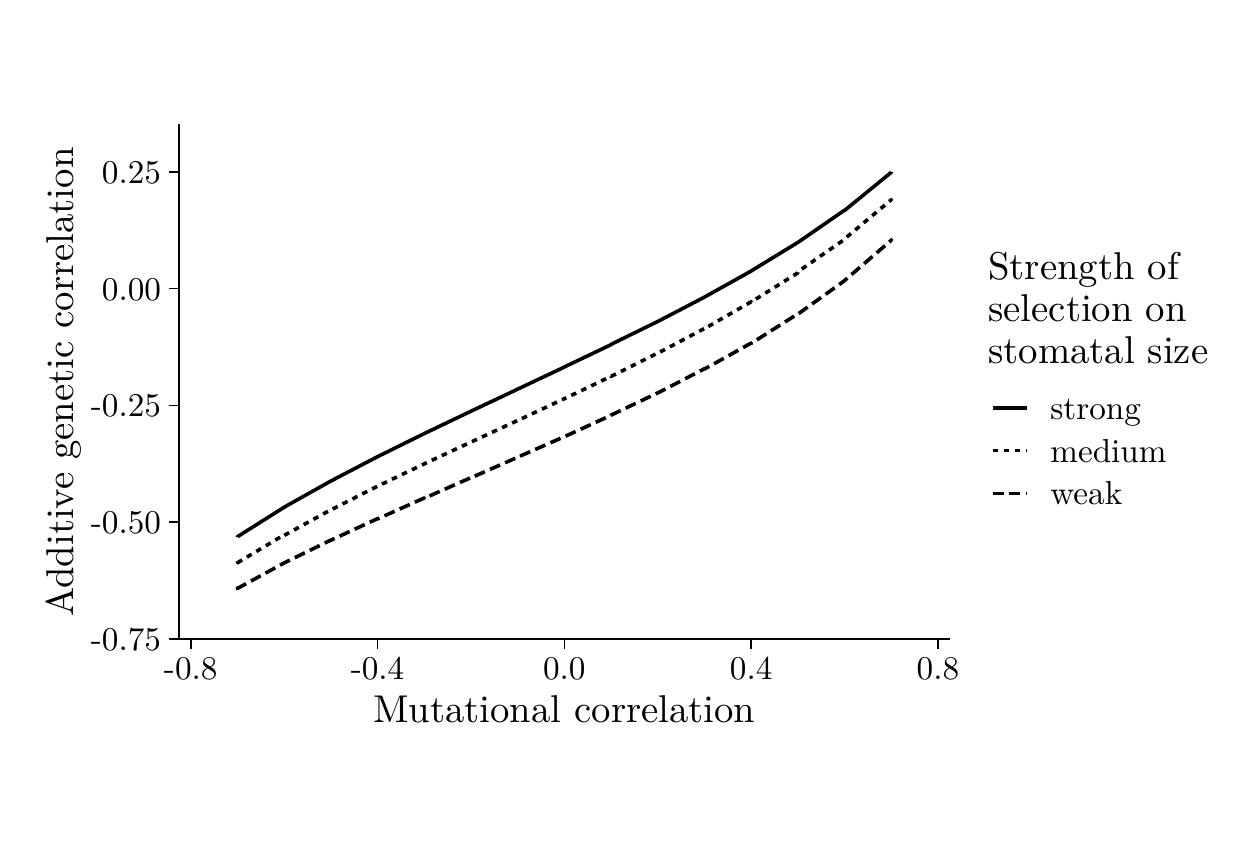
\begin{tikzpicture}[x=1pt,y=1pt]
\definecolor{fillColor}{RGB}{255,255,255}
\path[use as bounding box,fill=fillColor,fill opacity=0.00] (0,0) rectangle (433.62,289.08);
\begin{scope}
\path[clip] ( 54.69, 68.20) rectangle (333.15,253.84);
\definecolor{drawColor}{RGB}{0,0,0}

\path[draw=drawColor,line width= 1.3pt,line join=round] ( 75.79,105.11) --
	( 75.79,105.13) --
	( 75.79,105.14) --
	( 92.66,115.77) --
	( 92.66,115.79) --
	( 92.66,115.79) --
	(109.54,125.26) --
	(109.54,125.29) --
	(109.54,125.24) --
	(126.42,134.06) --
	(126.42,134.06) --
	(126.42,134.05) --
	(143.29,142.40) --
	(143.29,142.40) --
	(143.29,142.40) --
	(160.17,150.48) --
	(160.17,150.48) --
	(160.17,150.48) --
	(177.04,158.44) --
	(177.04,158.45) --
	(177.04,158.46) --
	(193.92,166.42) --
	(193.92,166.44) --
	(193.92,166.47) --
	(210.80,174.53) --
	(210.80,174.56) --
	(210.80,174.64) --
	(227.67,182.91) --
	(227.67,182.92) --
	(227.67,182.90) --
	(244.55,191.71) --
	(244.55,191.74) --
	(244.55,191.72) --
	(261.43,201.14) --
	(261.43,201.20) --
	(261.43,201.15) --
	(278.30,211.48) --
	(278.30,211.48) --
	(278.30,211.46) --
	(295.18,223.14) --
	(295.18,223.17) --
	(295.18,223.02) --
	(312.06,236.81) --
	(312.06,236.87) --
	(312.06,236.94);

\path[draw=drawColor,line width= 1.3pt,dash pattern=on 2pt off 2pt ,line join=round] ( 75.79, 95.71) --
	( 75.79, 95.70) --
	( 75.79, 95.71) --
	( 92.66,105.80) --
	( 92.66,105.82) --
	( 92.66,105.60) --
	(109.54,114.87) --
	(109.54,114.88) --
	(109.54,114.82) --
	(126.42,123.39) --
	(126.42,123.36) --
	(126.42,123.38) --
	(143.29,131.45) --
	(143.29,131.48) --
	(143.29,131.47) --
	(160.17,139.33) --
	(160.17,139.32) --
	(160.17,139.32) --
	(177.04,147.13) --
	(177.04,147.18) --
	(177.04,147.12) --
	(193.92,155.01) --
	(193.92,155.15) --
	(193.92,154.99) --
	(210.80,163.08) --
	(210.80,163.10) --
	(210.80,163.05) --
	(227.67,171.48) --
	(227.67,171.53) --
	(227.67,171.43) --
	(244.55,180.38) --
	(244.55,180.46) --
	(244.55,180.29) --
	(261.43,190.03) --
	(261.43,189.95) --
	(261.43,189.93) --
	(278.30,200.48) --
	(278.30,200.58) --
	(278.30,200.88) --
	(295.18,212.57) --
	(295.18,212.72) --
	(295.18,212.74) --
	(312.06,226.91) --
	(312.06,226.99) --
	(312.06,226.84);

\path[draw=drawColor,line width= 1.3pt,dash pattern=on 4pt off 2pt ,line join=round] ( 75.79, 86.47) --
	( 75.79, 86.67) --
	( 75.79, 86.44) --
	( 92.66, 95.65) --
	( 92.66, 95.67) --
	( 92.66, 95.66) --
	(109.54,103.91) --
	(109.54,103.90) --
	(109.54,103.87) --
	(126.42,111.66) --
	(126.42,111.67) --
	(126.42,111.55) --
	(143.29,119.13) --
	(143.29,119.15) --
	(143.29,119.01) --
	(160.17,126.49) --
	(160.17,126.52) --
	(160.17,126.40) --
	(177.04,133.86) --
	(177.04,133.92) --
	(177.04,133.87) --
	(193.92,141.29) --
	(193.92,141.28) --
	(193.92,141.27) --
	(210.80,149.00) --
	(210.80,149.00) --
	(210.80,149.06) --
	(227.67,157.11) --
	(227.67,157.10) --
	(227.67,157.07) --
	(244.55,165.83) --
	(244.55,165.75) --
	(244.55,165.70) --
	(261.43,175.11) --
	(261.43,175.15) --
	(261.43,174.98) --
	(278.30,185.67) --
	(278.30,185.67) --
	(278.30,185.55) --
	(295.18,197.66) --
	(295.18,197.81) --
	(295.18,197.70) --
	(312.06,212.27) --
	(312.06,212.52) --
	(312.06,212.47);
\end{scope}
\begin{scope}
\path[clip] (  0.00,  0.00) rectangle (433.62,289.08);
\definecolor{drawColor}{RGB}{0,0,0}

\path[draw=drawColor,line width= 0.6pt,line join=round,line cap=rect] ( 54.69, 68.20) --
	( 54.69,253.84);
\end{scope}
\begin{scope}
\path[clip] (  0.00,  0.00) rectangle (433.62,289.08);
\definecolor{drawColor}{RGB}{0,0,0}

\node[text=drawColor,anchor=base east,inner sep=0pt, outer sep=0pt, scale=  1.20] at ( 48.19, 64.07) {-0.75};

\node[text=drawColor,anchor=base east,inner sep=0pt, outer sep=0pt, scale=  1.20] at ( 48.19,106.26) {-0.50};

\node[text=drawColor,anchor=base east,inner sep=0pt, outer sep=0pt, scale=  1.20] at ( 48.19,148.45) {-0.25};

\node[text=drawColor,anchor=base east,inner sep=0pt, outer sep=0pt, scale=  1.20] at ( 48.19,190.64) {0.00};

\node[text=drawColor,anchor=base east,inner sep=0pt, outer sep=0pt, scale=  1.20] at ( 48.19,232.83) {0.25};
\end{scope}
\begin{scope}
\path[clip] (  0.00,  0.00) rectangle (433.62,289.08);
\definecolor{drawColor}{RGB}{0,0,0}

\path[draw=drawColor,line width= 0.6pt,line join=round] ( 51.19, 68.20) --
	( 54.69, 68.20);

\path[draw=drawColor,line width= 0.6pt,line join=round] ( 51.19,110.39) --
	( 54.69,110.39);

\path[draw=drawColor,line width= 0.6pt,line join=round] ( 51.19,152.58) --
	( 54.69,152.58);

\path[draw=drawColor,line width= 0.6pt,line join=round] ( 51.19,194.77) --
	( 54.69,194.77);

\path[draw=drawColor,line width= 0.6pt,line join=round] ( 51.19,236.96) --
	( 54.69,236.96);
\end{scope}
\begin{scope}
\path[clip] (  0.00,  0.00) rectangle (433.62,289.08);
\definecolor{drawColor}{RGB}{0,0,0}

\path[draw=drawColor,line width= 0.6pt,line join=round,line cap=rect] ( 54.69, 68.20) --
	(333.15, 68.20);
\end{scope}
\begin{scope}
\path[clip] (  0.00,  0.00) rectangle (433.62,289.08);
\definecolor{drawColor}{RGB}{0,0,0}

\path[draw=drawColor,line width= 0.6pt,line join=round] ( 58.91, 64.70) --
	( 58.91, 68.20);

\path[draw=drawColor,line width= 0.6pt,line join=round] (126.42, 64.70) --
	(126.42, 68.20);

\path[draw=drawColor,line width= 0.6pt,line join=round] (193.92, 64.70) --
	(193.92, 68.20);

\path[draw=drawColor,line width= 0.6pt,line join=round] (261.43, 64.70) --
	(261.43, 68.20);

\path[draw=drawColor,line width= 0.6pt,line join=round] (328.93, 64.70) --
	(328.93, 68.20);
\end{scope}
\begin{scope}
\path[clip] (  0.00,  0.00) rectangle (433.62,289.08);
\definecolor{drawColor}{RGB}{0,0,0}

\node[text=drawColor,anchor=base,inner sep=0pt, outer sep=0pt, scale=  1.20] at ( 58.91, 53.44) {-0.8};

\node[text=drawColor,anchor=base,inner sep=0pt, outer sep=0pt, scale=  1.20] at (126.42, 53.44) {-0.4};

\node[text=drawColor,anchor=base,inner sep=0pt, outer sep=0pt, scale=  1.20] at (193.92, 53.44) {0.0};

\node[text=drawColor,anchor=base,inner sep=0pt, outer sep=0pt, scale=  1.20] at (261.43, 53.44) {0.4};

\node[text=drawColor,anchor=base,inner sep=0pt, outer sep=0pt, scale=  1.20] at (328.93, 53.44) {0.8};
\end{scope}
\begin{scope}
\path[clip] (  0.00,  0.00) rectangle (433.62,289.08);
\definecolor{drawColor}{RGB}{0,0,0}

\node[text=drawColor,anchor=base,inner sep=0pt, outer sep=0pt, scale=  1.40] at (193.92, 37.96) {Mutational correlation};
\end{scope}
\begin{scope}
\path[clip] (  0.00,  0.00) rectangle (433.62,289.08);
\definecolor{drawColor}{RGB}{0,0,0}

\node[text=drawColor,rotate= 90.00,anchor=base,inner sep=0pt, outer sep=0pt, scale=  1.40] at ( 16.64,161.02) {Additive genetic correlation};
\end{scope}
\begin{scope}
\path[clip] (  0.00,  0.00) rectangle (433.62,289.08);
\definecolor{drawColor}{RGB}{0,0,0}

\node[text=drawColor,anchor=base west,inner sep=0pt, outer sep=0pt, scale=  1.40] at (347.15,197.92) {Strength of};

\node[text=drawColor,anchor=base west,inner sep=0pt, outer sep=0pt, scale=  1.40] at (347.15,182.80) {selection on};

\node[text=drawColor,anchor=base west,inner sep=0pt, outer sep=0pt, scale=  1.40] at (347.15,167.68) {stomatal size};
\end{scope}
\begin{scope}
\path[clip] (  0.00,  0.00) rectangle (433.62,289.08);
\definecolor{drawColor}{RGB}{0,0,0}

\path[draw=drawColor,line width= 1.3pt,line join=round] (348.69,151.62) -- (361.01,151.62);
\end{scope}
\begin{scope}
\path[clip] (  0.00,  0.00) rectangle (433.62,289.08);
\definecolor{drawColor}{RGB}{0,0,0}

\path[draw=drawColor,line width= 1.3pt,dash pattern=on 2pt off 2pt ,line join=round] (348.69,136.22) -- (361.01,136.22);
\end{scope}
\begin{scope}
\path[clip] (  0.00,  0.00) rectangle (433.62,289.08);
\definecolor{drawColor}{RGB}{0,0,0}

\path[draw=drawColor,line width= 1.3pt,dash pattern=on 4pt off 2pt ,line join=round] (348.69,120.82) -- (361.01,120.82);
\end{scope}
\begin{scope}
\path[clip] (  0.00,  0.00) rectangle (433.62,289.08);
\definecolor{drawColor}{RGB}{0,0,0}

\node[text=drawColor,anchor=base west,inner sep=0pt, outer sep=0pt, scale=  1.20] at (369.55,147.49) {strong};
\end{scope}
\begin{scope}
\path[clip] (  0.00,  0.00) rectangle (433.62,289.08);
\definecolor{drawColor}{RGB}{0,0,0}

\node[text=drawColor,anchor=base west,inner sep=0pt, outer sep=0pt, scale=  1.20] at (369.55,132.09) {medium};
\end{scope}
\begin{scope}
\path[clip] (  0.00,  0.00) rectangle (433.62,289.08);
\definecolor{drawColor}{RGB}{0,0,0}

\node[text=drawColor,anchor=base west,inner sep=0pt, outer sep=0pt, scale=  1.20] at (369.55,116.69) {weak};
\end{scope}
\end{tikzpicture}

\end{figure}

\newpage

\begin{figure}
\caption{The effect of selection on and mutational variance in stomatal size on the additive genetic variance under $H_3$: stomatal adaptation + bounded size hypothesis. The ratio of additive genetic variance within species at mutation-selection balance in stomatal density and size depends on the relative mutational variance ($M_{d_\mathrm{S}} / M_{a_\mathrm{S}}$) and the strength of selection on stomatal size ($\phi_a \omega$). Results are shown for $M_{d_\mathrm{S}} = 3.77 \times 10^{-7}$ while $M_{a_\mathrm{S}}$ varied from $0.1 M_{d_\mathrm{S}}$ (low, solid line), $M_{d_\mathrm{S}}$ (medium, dotted line), and $10 M_{d_\mathrm{S}}$ (high, dashed line). The relative strength of selection on stomatal size varied between $\phi_a = 0.5$ and 2. We also assumed no mutational correlation and $\omega = 3.77 \times 10^{-2}$. See text for explanation of parameter values.}
% Created by tikzDevice version 0.12.6 on 2025-08-19 18:47:28
% !TEX encoding = UTF-8 Unicode
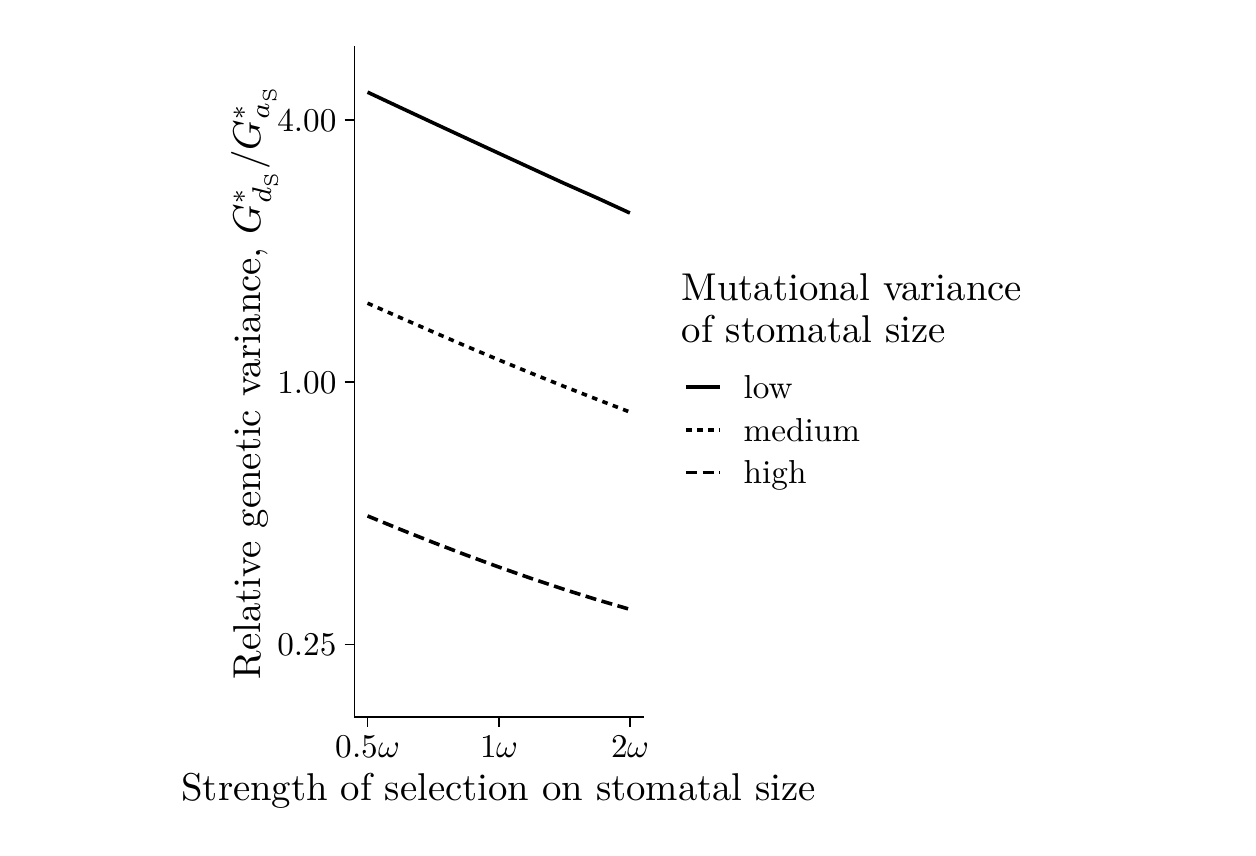
\begin{tikzpicture}[x=1pt,y=1pt]
\definecolor{fillColor}{RGB}{255,255,255}
\path[use as bounding box,fill=fillColor,fill opacity=0.00] (0,0) rectangle (433.62,289.08);
\begin{scope}
\path[clip] (118.07, 39.96) rectangle (222.34,282.08);
\definecolor{drawColor}{RGB}{0,0,0}

\path[draw=drawColor,line width= 1.3pt,line join=round] (122.81,265.77) --
	(134.66,260.21) --
	(146.51,254.68) --
	(158.36,249.18) --
	(170.21,243.70) --
	(182.06,238.24) --
	(193.91,232.80) --
	(205.76,227.55) --
	(217.60,222.11);

\path[draw=drawColor,line width= 1.3pt,dash pattern=on 2pt off 2pt ,line join=round] (122.81,189.52) --
	(134.66,184.30) --
	(146.51,179.13) --
	(158.36,174.02) --
	(170.21,169.04) --
	(182.06,164.18) --
	(193.91,159.41) --
	(205.76,154.76) --
	(217.60,150.19);

\path[draw=drawColor,line width= 1.3pt,dash pattern=on 4pt off 2pt ,line join=round] (122.81,112.64) --
	(134.66,107.78) --
	(146.51,103.08) --
	(158.36, 98.54) --
	(170.21, 94.19) --
	(182.06, 90.03) --
	(193.91, 86.08) --
	(205.76, 82.36) --
	(217.60, 78.89);
\end{scope}
\begin{scope}
\path[clip] (  0.00,  0.00) rectangle (433.62,289.08);
\definecolor{drawColor}{RGB}{0,0,0}

\path[draw=drawColor,line width= 0.6pt,line join=round,line cap=rect] (118.07, 39.96) --
	(118.07,282.08);
\end{scope}
\begin{scope}
\path[clip] (  0.00,  0.00) rectangle (433.62,289.08);
\definecolor{drawColor}{RGB}{0,0,0}

\node[text=drawColor,anchor=base east,inner sep=0pt, outer sep=0pt, scale=  1.20] at (111.57, 62.09) {0.25};

\node[text=drawColor,anchor=base east,inner sep=0pt, outer sep=0pt, scale=  1.20] at (111.57,156.89) {1.00};

\node[text=drawColor,anchor=base east,inner sep=0pt, outer sep=0pt, scale=  1.20] at (111.57,251.68) {4.00};
\end{scope}
\begin{scope}
\path[clip] (  0.00,  0.00) rectangle (433.62,289.08);
\definecolor{drawColor}{RGB}{0,0,0}

\path[draw=drawColor,line width= 0.6pt,line join=round] (114.57, 66.23) --
	(118.07, 66.23);

\path[draw=drawColor,line width= 0.6pt,line join=round] (114.57,161.02) --
	(118.07,161.02);

\path[draw=drawColor,line width= 0.6pt,line join=round] (114.57,255.82) --
	(118.07,255.82);
\end{scope}
\begin{scope}
\path[clip] (  0.00,  0.00) rectangle (433.62,289.08);
\definecolor{drawColor}{RGB}{0,0,0}

\path[draw=drawColor,line width= 0.6pt,line join=round,line cap=rect] (118.07, 39.96) --
	(222.34, 39.96);
\end{scope}
\begin{scope}
\path[clip] (  0.00,  0.00) rectangle (433.62,289.08);
\definecolor{drawColor}{RGB}{0,0,0}

\path[draw=drawColor,line width= 0.6pt,line join=round] (122.81, 36.46) --
	(122.81, 39.96);

\path[draw=drawColor,line width= 0.6pt,line join=round] (170.21, 36.46) --
	(170.21, 39.96);

\path[draw=drawColor,line width= 0.6pt,line join=round] (217.60, 36.46) --
	(217.60, 39.96);
\end{scope}
\begin{scope}
\path[clip] (  0.00,  0.00) rectangle (433.62,289.08);
\definecolor{drawColor}{RGB}{0,0,0}

\node[text=drawColor,anchor=base,inner sep=0pt, outer sep=0pt, scale=  1.20] at (122.81, 25.20) {$0.5\omega$};

\node[text=drawColor,anchor=base,inner sep=0pt, outer sep=0pt, scale=  1.20] at (170.21, 25.20) {$1\omega$};

\node[text=drawColor,anchor=base,inner sep=0pt, outer sep=0pt, scale=  1.20] at (217.60, 25.20) {$2\omega$};
\end{scope}
\begin{scope}
\path[clip] (  0.00,  0.00) rectangle (433.62,289.08);
\definecolor{drawColor}{RGB}{0,0,0}

\node[text=drawColor,anchor=base,inner sep=0pt, outer sep=0pt, scale=  1.40] at (170.21,  9.72) {Strength of selection on stomatal size};
\end{scope}
\begin{scope}
\path[clip] (  0.00,  0.00) rectangle (433.62,289.08);
\definecolor{drawColor}{RGB}{0,0,0}

\node[text=drawColor,rotate= 90.00,anchor=base,inner sep=0pt, outer sep=0pt, scale=  1.40] at ( 84.02,161.02) {Relative genetic variance, $G^*_{d_\mathrm{S}} / G^*_{a_\mathrm{S}}$};
\end{scope}
\begin{scope}
\path[clip] (  0.00,  0.00) rectangle (433.62,289.08);
\definecolor{drawColor}{RGB}{0,0,0}

\node[text=drawColor,anchor=base west,inner sep=0pt, outer sep=0pt, scale=  1.40] at (236.34,190.36) {Mutational variance};

\node[text=drawColor,anchor=base west,inner sep=0pt, outer sep=0pt, scale=  1.40] at (236.34,175.24) {of stomatal size};
\end{scope}
\begin{scope}
\path[clip] (  0.00,  0.00) rectangle (433.62,289.08);
\definecolor{drawColor}{RGB}{0,0,0}

\path[draw=drawColor,line width= 1.3pt,line join=round] (237.88,159.18) -- (250.20,159.18);
\end{scope}
\begin{scope}
\path[clip] (  0.00,  0.00) rectangle (433.62,289.08);
\definecolor{drawColor}{RGB}{0,0,0}

\path[draw=drawColor,line width= 1.3pt,dash pattern=on 2pt off 2pt ,line join=round] (237.88,143.78) -- (250.20,143.78);
\end{scope}
\begin{scope}
\path[clip] (  0.00,  0.00) rectangle (433.62,289.08);
\definecolor{drawColor}{RGB}{0,0,0}

\path[draw=drawColor,line width= 1.3pt,dash pattern=on 4pt off 2pt ,line join=round] (237.88,128.38) -- (250.20,128.38);
\end{scope}
\begin{scope}
\path[clip] (  0.00,  0.00) rectangle (433.62,289.08);
\definecolor{drawColor}{RGB}{0,0,0}

\node[text=drawColor,anchor=base west,inner sep=0pt, outer sep=0pt, scale=  1.20] at (258.74,155.05) {low};
\end{scope}
\begin{scope}
\path[clip] (  0.00,  0.00) rectangle (433.62,289.08);
\definecolor{drawColor}{RGB}{0,0,0}

\node[text=drawColor,anchor=base west,inner sep=0pt, outer sep=0pt, scale=  1.20] at (258.74,139.65) {medium};
\end{scope}
\begin{scope}
\path[clip] (  0.00,  0.00) rectangle (433.62,289.08);
\definecolor{drawColor}{RGB}{0,0,0}

\node[text=drawColor,anchor=base west,inner sep=0pt, outer sep=0pt, scale=  1.20] at (258.74,124.25) {high};
\end{scope}
\end{tikzpicture}

\end{figure}

\newpage

\begin{figure}
\caption{The predicted response to selection on greater $g_\mathrm{s,max}$ under three hypotheses: $H_2$: stomatal-area adaptation (blue); $H_1$: stomatal-area minimization (green); and $H_3$: stomatal adaptation + bounded size (red). Each vector shows the relative response of stomatal density (log-scale, $x$-axis) and stomatal size (log-scale, $y$-axis). The predicted response assumes the additive genetic variance is at equilibrium and there is no other change in parameters from the baseline scenario described in the Supporting Information. The left and right panels show how mutational correlation between stomatal density and size affect the response vectors.}
% Created by tikzDevice version 0.12.6 on 2025-05-24 13:23:51
% !TEX encoding = UTF-8 Unicode
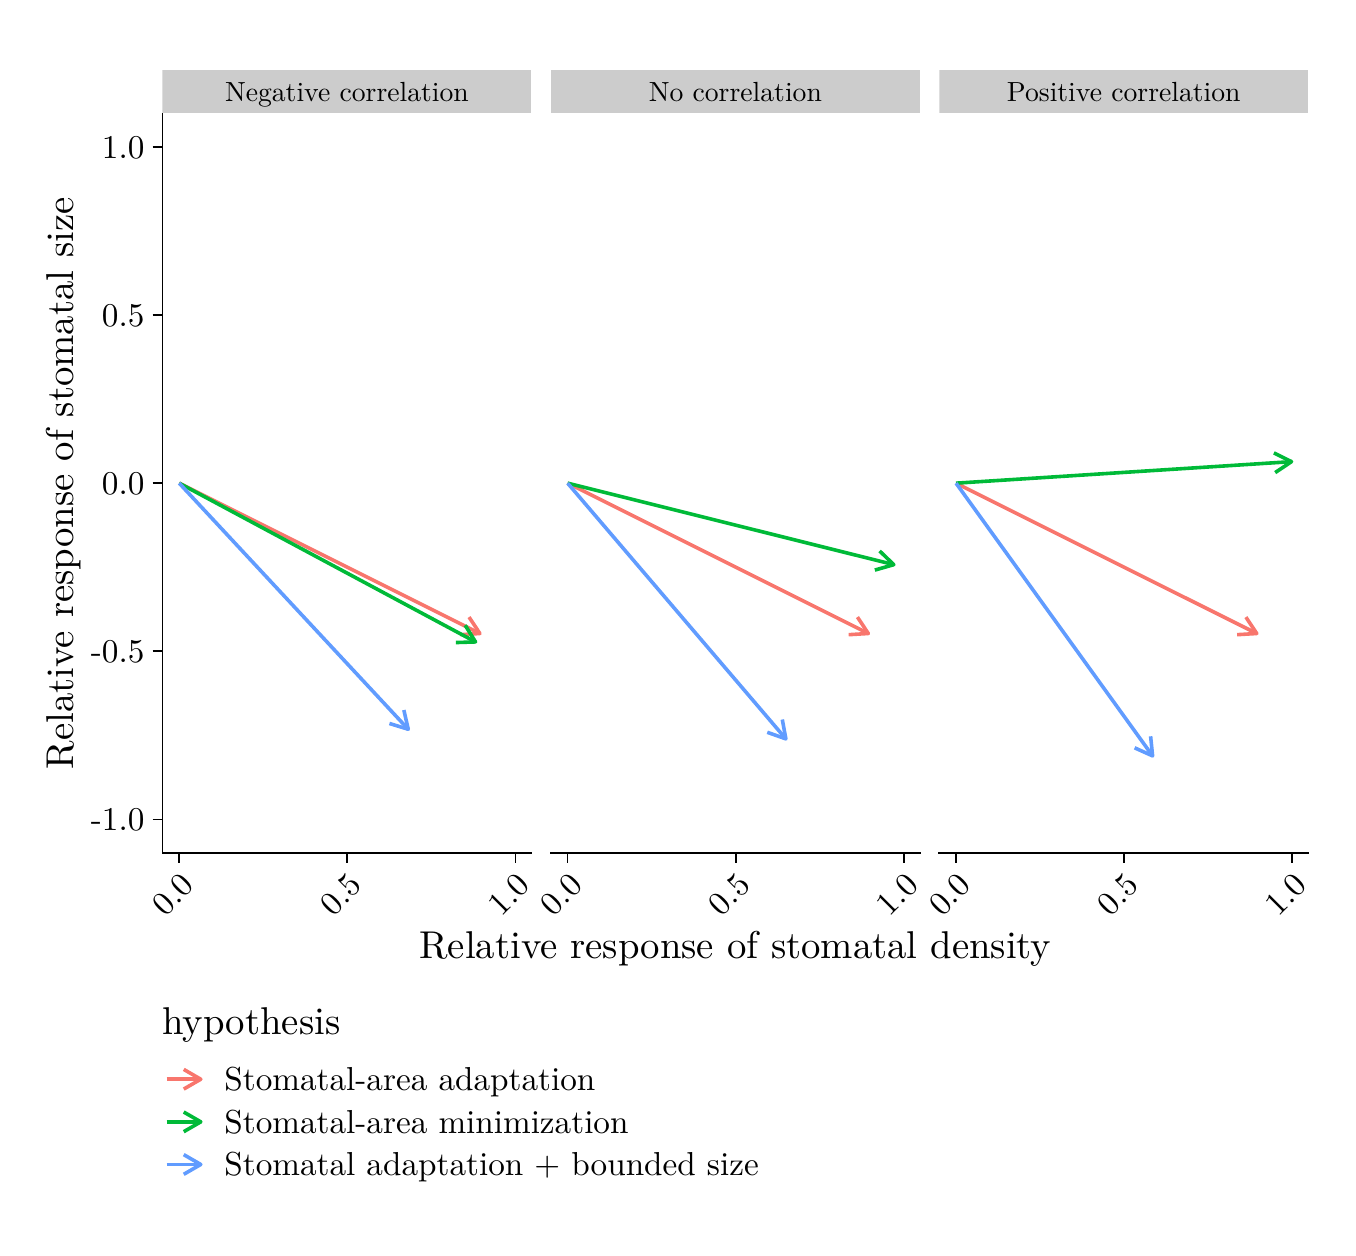
\begin{tikzpicture}[x=1pt,y=1pt]
\definecolor{fillColor}{RGB}{255,255,255}
\path[use as bounding box,fill=fillColor,fill opacity=0.00] (0,0) rectangle (469.75,433.62);
\begin{scope}
\path[clip] ( 48.69,135.40) rectangle (182.05,402.65);
\definecolor{drawColor}{RGB}{248,118,109}

\path[draw=drawColor,line width= 1.3pt,line join=round] ( 54.75,269.02) -- (163.41,214.70);

\path[draw=drawColor,line width= 1.3pt,line join=round] (156.31,214.27) --
	(163.41,214.70) --
	(159.49,220.63);
\definecolor{drawColor}{RGB}{0,186,56}

\path[draw=drawColor,line width= 1.3pt,line join=round] ( 54.75,269.02) -- (161.83,211.66);

\path[draw=drawColor,line width= 1.3pt,line join=round] (154.73,211.43) --
	(161.83,211.66) --
	(158.08,217.70);
\definecolor{drawColor}{RGB}{97,156,255}

\path[draw=drawColor,line width= 1.3pt,line join=round] ( 54.75,269.02) -- (137.52,180.10);

\path[draw=drawColor,line width= 1.3pt,line join=round] (130.72,182.19) --
	(137.52,180.10) --
	(135.93,187.04);
\end{scope}
\begin{scope}
\path[clip] (189.05,135.40) rectangle (322.40,402.65);
\definecolor{drawColor}{RGB}{248,118,109}

\path[draw=drawColor,line width= 1.3pt,line join=round] (195.11,269.02) -- (303.76,214.70);

\path[draw=drawColor,line width= 1.3pt,line join=round] (296.66,214.27) --
	(303.76,214.70) --
	(299.84,220.63);
\definecolor{drawColor}{RGB}{0,186,56}

\path[draw=drawColor,line width= 1.3pt,line join=round] (195.11,269.02) -- (312.97,239.58);

\path[draw=drawColor,line width= 1.3pt,line join=round] (306.13,237.62) --
	(312.97,239.58) --
	(307.85,244.52);
\definecolor{drawColor}{RGB}{97,156,255}

\path[draw=drawColor,line width= 1.3pt,line join=round] (195.11,269.02) -- (273.97,176.62);

\path[draw=drawColor,line width= 1.3pt,line join=round] (267.26,179.00) --
	(273.97,176.62) --
	(272.68,183.62);
\end{scope}
\begin{scope}
\path[clip] (329.40,135.40) rectangle (462.76,402.65);
\definecolor{drawColor}{RGB}{248,118,109}

\path[draw=drawColor,line width= 1.3pt,line join=round] (335.46,269.02) -- (444.12,214.70);

\path[draw=drawColor,line width= 1.3pt,line join=round] (437.02,214.27) --
	(444.12,214.70) --
	(440.20,220.63);
\definecolor{drawColor}{RGB}{0,186,56}

\path[draw=drawColor,line width= 1.3pt,line join=round] (335.46,269.02) -- (456.69,276.80);

\path[draw=drawColor,line width= 1.3pt,line join=round] (450.77,272.85) --
	(456.69,276.80) --
	(450.32,279.95);
\definecolor{drawColor}{RGB}{97,156,255}

\path[draw=drawColor,line width= 1.3pt,line join=round] (335.46,269.02) -- (406.49,170.47);

\path[draw=drawColor,line width= 1.3pt,line join=round] (400.00,173.39) --
	(406.49,170.47) --
	(405.77,177.55);
\end{scope}
\begin{scope}
\path[clip] ( 48.69,402.65) rectangle (182.05,418.48);
\definecolor{fillColor}{gray}{0.80}

\path[fill=fillColor] ( 48.69,402.65) rectangle (182.05,418.48);
\definecolor{drawColor}{RGB}{0,0,0}

\node[text=drawColor,anchor=base,inner sep=0pt, outer sep=0pt, scale=  1.00] at (115.37,407.12) {Negative correlation};
\end{scope}
\begin{scope}
\path[clip] (189.05,402.65) rectangle (322.40,418.48);
\definecolor{fillColor}{gray}{0.80}

\path[fill=fillColor] (189.05,402.65) rectangle (322.40,418.48);
\definecolor{drawColor}{RGB}{0,0,0}

\node[text=drawColor,anchor=base,inner sep=0pt, outer sep=0pt, scale=  1.00] at (255.72,407.12) {No correlation};
\end{scope}
\begin{scope}
\path[clip] (329.40,402.65) rectangle (462.76,418.48);
\definecolor{fillColor}{gray}{0.80}

\path[fill=fillColor] (329.40,402.65) rectangle (462.75,418.48);
\definecolor{drawColor}{RGB}{0,0,0}

\node[text=drawColor,anchor=base,inner sep=0pt, outer sep=0pt, scale=  1.00] at (396.08,407.12) {Positive correlation};
\end{scope}
\begin{scope}
\path[clip] (  0.00,  0.00) rectangle (469.75,433.62);
\definecolor{drawColor}{RGB}{0,0,0}

\path[draw=drawColor,line width= 0.6pt,line join=round,line cap=rect] ( 48.69,135.40) --
	(182.05,135.40);
\end{scope}
\begin{scope}
\path[clip] (  0.00,  0.00) rectangle (469.75,433.62);
\definecolor{drawColor}{RGB}{0,0,0}

\path[draw=drawColor,line width= 0.6pt,line join=round] ( 54.75,131.90) --
	( 54.75,135.40);

\path[draw=drawColor,line width= 0.6pt,line join=round] (115.49,131.90) --
	(115.49,135.40);

\path[draw=drawColor,line width= 0.6pt,line join=round] (176.23,131.90) --
	(176.23,135.40);
\end{scope}
\begin{scope}
\path[clip] (  0.00,  0.00) rectangle (469.75,433.62);
\definecolor{drawColor}{RGB}{0,0,0}

\node[text=drawColor,rotate= 45.00,anchor=base east,inner sep=0pt, outer sep=0pt, scale=  1.20] at ( 60.60,123.05) {0.0};

\node[text=drawColor,rotate= 45.00,anchor=base east,inner sep=0pt, outer sep=0pt, scale=  1.20] at (121.34,123.05) {0.5};

\node[text=drawColor,rotate= 45.00,anchor=base east,inner sep=0pt, outer sep=0pt, scale=  1.20] at (182.08,123.05) {1.0};
\end{scope}
\begin{scope}
\path[clip] (  0.00,  0.00) rectangle (469.75,433.62);
\definecolor{drawColor}{RGB}{0,0,0}

\path[draw=drawColor,line width= 0.6pt,line join=round,line cap=rect] (189.05,135.40) --
	(322.40,135.40);
\end{scope}
\begin{scope}
\path[clip] (  0.00,  0.00) rectangle (469.75,433.62);
\definecolor{drawColor}{RGB}{0,0,0}

\path[draw=drawColor,line width= 0.6pt,line join=round] (195.11,131.90) --
	(195.11,135.40);

\path[draw=drawColor,line width= 0.6pt,line join=round] (255.85,131.90) --
	(255.85,135.40);

\path[draw=drawColor,line width= 0.6pt,line join=round] (316.59,131.90) --
	(316.59,135.40);
\end{scope}
\begin{scope}
\path[clip] (  0.00,  0.00) rectangle (469.75,433.62);
\definecolor{drawColor}{RGB}{0,0,0}

\node[text=drawColor,rotate= 45.00,anchor=base east,inner sep=0pt, outer sep=0pt, scale=  1.20] at (200.95,123.05) {0.0};

\node[text=drawColor,rotate= 45.00,anchor=base east,inner sep=0pt, outer sep=0pt, scale=  1.20] at (261.69,123.05) {0.5};

\node[text=drawColor,rotate= 45.00,anchor=base east,inner sep=0pt, outer sep=0pt, scale=  1.20] at (322.43,123.05) {1.0};
\end{scope}
\begin{scope}
\path[clip] (  0.00,  0.00) rectangle (469.75,433.62);
\definecolor{drawColor}{RGB}{0,0,0}

\path[draw=drawColor,line width= 0.6pt,line join=round,line cap=rect] (329.40,135.40) --
	(462.76,135.40);
\end{scope}
\begin{scope}
\path[clip] (  0.00,  0.00) rectangle (469.75,433.62);
\definecolor{drawColor}{RGB}{0,0,0}

\path[draw=drawColor,line width= 0.6pt,line join=round] (335.46,131.90) --
	(335.46,135.40);

\path[draw=drawColor,line width= 0.6pt,line join=round] (396.20,131.90) --
	(396.20,135.40);

\path[draw=drawColor,line width= 0.6pt,line join=round] (456.94,131.90) --
	(456.94,135.40);
\end{scope}
\begin{scope}
\path[clip] (  0.00,  0.00) rectangle (469.75,433.62);
\definecolor{drawColor}{RGB}{0,0,0}

\node[text=drawColor,rotate= 45.00,anchor=base east,inner sep=0pt, outer sep=0pt, scale=  1.20] at (341.31,123.05) {0.0};

\node[text=drawColor,rotate= 45.00,anchor=base east,inner sep=0pt, outer sep=0pt, scale=  1.20] at (402.05,123.05) {0.5};

\node[text=drawColor,rotate= 45.00,anchor=base east,inner sep=0pt, outer sep=0pt, scale=  1.20] at (462.79,123.05) {1.0};
\end{scope}
\begin{scope}
\path[clip] (  0.00,  0.00) rectangle (469.75,433.62);
\definecolor{drawColor}{RGB}{0,0,0}

\path[draw=drawColor,line width= 0.6pt,line join=round,line cap=rect] ( 48.69,135.40) --
	( 48.69,402.65);
\end{scope}
\begin{scope}
\path[clip] (  0.00,  0.00) rectangle (469.75,433.62);
\definecolor{drawColor}{RGB}{0,0,0}

\node[text=drawColor,anchor=base east,inner sep=0pt, outer sep=0pt, scale=  1.20] at ( 42.19,143.41) {-1.0};

\node[text=drawColor,anchor=base east,inner sep=0pt, outer sep=0pt, scale=  1.20] at ( 42.19,204.15) {-0.5};

\node[text=drawColor,anchor=base east,inner sep=0pt, outer sep=0pt, scale=  1.20] at ( 42.19,264.89) {0.0};

\node[text=drawColor,anchor=base east,inner sep=0pt, outer sep=0pt, scale=  1.20] at ( 42.19,325.63) {0.5};

\node[text=drawColor,anchor=base east,inner sep=0pt, outer sep=0pt, scale=  1.20] at ( 42.19,386.37) {1.0};
\end{scope}
\begin{scope}
\path[clip] (  0.00,  0.00) rectangle (469.75,433.62);
\definecolor{drawColor}{RGB}{0,0,0}

\path[draw=drawColor,line width= 0.6pt,line join=round] ( 45.19,147.54) --
	( 48.69,147.54);

\path[draw=drawColor,line width= 0.6pt,line join=round] ( 45.19,208.28) --
	( 48.69,208.28);

\path[draw=drawColor,line width= 0.6pt,line join=round] ( 45.19,269.02) --
	( 48.69,269.02);

\path[draw=drawColor,line width= 0.6pt,line join=round] ( 45.19,329.76) --
	( 48.69,329.76);

\path[draw=drawColor,line width= 0.6pt,line join=round] ( 45.19,390.50) --
	( 48.69,390.50);
\end{scope}
\begin{scope}
\path[clip] (  0.00,  0.00) rectangle (469.75,433.62);
\definecolor{drawColor}{RGB}{0,0,0}

\node[text=drawColor,anchor=base,inner sep=0pt, outer sep=0pt, scale=  1.40] at (255.72, 97.42) {Relative response of stomatal density};
\end{scope}
\begin{scope}
\path[clip] (  0.00,  0.00) rectangle (469.75,433.62);
\definecolor{drawColor}{RGB}{0,0,0}

\node[text=drawColor,rotate= 90.00,anchor=base,inner sep=0pt, outer sep=0pt, scale=  1.40] at ( 16.64,269.02) {Relative response of stomatal size};
\end{scope}
\begin{scope}
\path[clip] (  0.00,  0.00) rectangle (469.75,433.62);
\definecolor{drawColor}{RGB}{0,0,0}

\node[text=drawColor,anchor=base west,inner sep=0pt, outer sep=0pt, scale=  1.40] at ( 48.69, 69.70) {hypothesis};
\end{scope}
\begin{scope}
\path[clip] (  0.00,  0.00) rectangle (469.75,433.62);
\definecolor{drawColor}{RGB}{248,118,109}

\path[draw=drawColor,line width= 1.3pt,line join=round] ( 50.23, 53.64) -- ( 62.55, 53.64);

\path[draw=drawColor,line width= 1.3pt,line join=round] ( 56.39, 50.08) --
	( 62.55, 53.64) --
	( 56.39, 57.19);
\end{scope}
\begin{scope}
\path[clip] (  0.00,  0.00) rectangle (469.75,433.62);
\definecolor{drawColor}{RGB}{0,186,56}

\path[draw=drawColor,line width= 1.3pt,line join=round] ( 50.23, 38.24) -- ( 62.55, 38.24);

\path[draw=drawColor,line width= 1.3pt,line join=round] ( 56.39, 34.68) --
	( 62.55, 38.24) --
	( 56.39, 41.79);
\end{scope}
\begin{scope}
\path[clip] (  0.00,  0.00) rectangle (469.75,433.62);
\definecolor{drawColor}{RGB}{97,156,255}

\path[draw=drawColor,line width= 1.3pt,line join=round] ( 50.23, 22.84) -- ( 62.55, 22.84);

\path[draw=drawColor,line width= 1.3pt,line join=round] ( 56.39, 19.28) --
	( 62.55, 22.84) --
	( 56.39, 26.39);
\end{scope}
\begin{scope}
\path[clip] (  0.00,  0.00) rectangle (469.75,433.62);
\definecolor{drawColor}{RGB}{0,0,0}

\node[text=drawColor,anchor=base west,inner sep=0pt, outer sep=0pt, scale=  1.20] at ( 71.09, 49.50) {Stomatal-area adaptation};
\end{scope}
\begin{scope}
\path[clip] (  0.00,  0.00) rectangle (469.75,433.62);
\definecolor{drawColor}{RGB}{0,0,0}

\node[text=drawColor,anchor=base west,inner sep=0pt, outer sep=0pt, scale=  1.20] at ( 71.09, 34.10) {Stomatal-area minimization};
\end{scope}
\begin{scope}
\path[clip] (  0.00,  0.00) rectangle (469.75,433.62);
\definecolor{drawColor}{RGB}{0,0,0}

\node[text=drawColor,anchor=base west,inner sep=0pt, outer sep=0pt, scale=  1.20] at ( 71.09, 18.70) {Stomatal adaptation + bounded size};
\end{scope}
\end{tikzpicture}

\end{figure}

\newpage

\begin{figure}
\caption{(Caption on next page.)}
% Created by tikzDevice version 0.12.6 on 2025-05-24 13:23:59
% !TEX encoding = UTF-8 Unicode
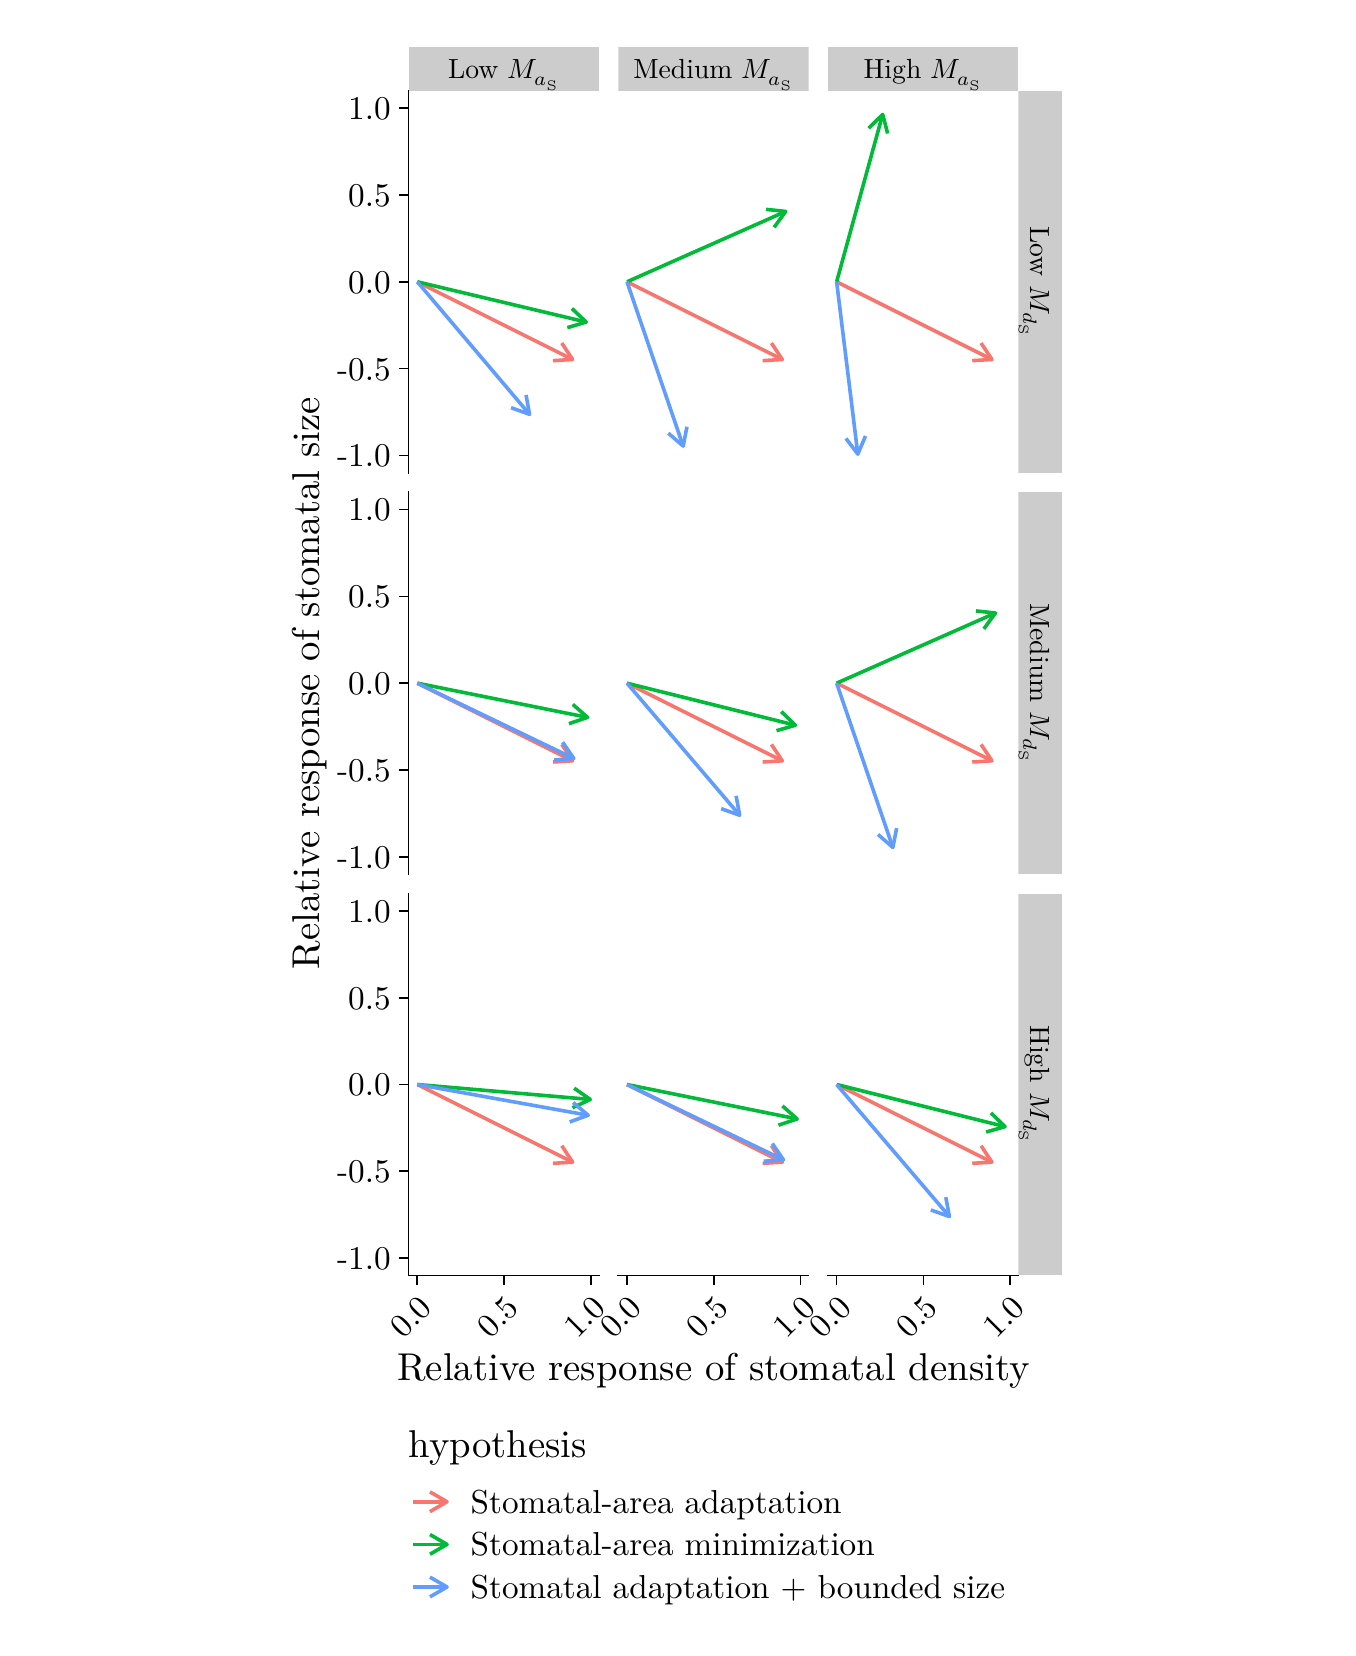
\begin{tikzpicture}[x=1pt,y=1pt]
\definecolor{fillColor}{RGB}{255,255,255}
\path[use as bounding box,fill=fillColor,fill opacity=0.00] (0,0) rectangle (469.75,578.16);
\begin{scope}
\path[clip] (137.67,417.31) rectangle (206.43,555.33);
\definecolor{drawColor}{RGB}{248,118,109}

\path[draw=drawColor,line width= 1.3pt,line join=round] (140.80,486.32) -- (196.91,458.26);

\path[draw=drawColor,line width= 1.3pt,line join=round] (189.81,457.83) --
	(196.91,458.26) --
	(192.99,464.20);
\definecolor{drawColor}{RGB}{0,186,56}

\path[draw=drawColor,line width= 1.3pt,line join=round] (140.80,486.32) -- (201.83,471.78);

\path[draw=drawColor,line width= 1.3pt,line join=round] (195.01,469.75) --
	(201.83,471.78) --
	(196.66,476.67);
\definecolor{drawColor}{RGB}{97,156,255}

\path[draw=drawColor,line width= 1.3pt,line join=round] (140.80,486.32) -- (181.35,438.44);

\path[draw=drawColor,line width= 1.3pt,line join=round] (174.65,440.85) --
	(181.35,438.44) --
	(180.08,445.44);
\end{scope}
\begin{scope}
\path[clip] (137.67,272.28) rectangle (206.43,410.31);
\definecolor{drawColor}{RGB}{248,118,109}

\path[draw=drawColor,line width= 1.3pt,line join=round] (140.80,341.29) -- (196.91,313.24);

\path[draw=drawColor,line width= 1.3pt,line join=round] (189.81,312.81) --
	(196.91,313.24) --
	(192.99,319.17);
\definecolor{drawColor}{RGB}{0,186,56}

\path[draw=drawColor,line width= 1.3pt,line join=round] (140.80,341.29) -- (202.31,328.93);

\path[draw=drawColor,line width= 1.3pt,line join=round] (195.57,326.65) --
	(202.31,328.93) --
	(196.97,333.63);
\definecolor{drawColor}{RGB}{97,156,255}

\path[draw=drawColor,line width= 1.3pt,line join=round] (140.80,341.29) -- (197.33,314.08);

\path[draw=drawColor,line width= 1.3pt,line join=round] (190.24,313.55) --
	(197.33,314.08) --
	(193.32,319.96);
\end{scope}
\begin{scope}
\path[clip] (137.67,127.26) rectangle (206.43,265.28);
\definecolor{drawColor}{RGB}{248,118,109}

\path[draw=drawColor,line width= 1.3pt,line join=round] (140.80,196.27) -- (196.91,168.21);

\path[draw=drawColor,line width= 1.3pt,line join=round] (189.81,167.79) --
	(196.91,168.21) --
	(192.99,174.15);
\definecolor{drawColor}{RGB}{0,186,56}

\path[draw=drawColor,line width= 1.3pt,line join=round] (140.80,196.27) -- (203.30,190.87);

\path[draw=drawColor,line width= 1.3pt,line join=round] (196.86,187.86) --
	(203.30,190.87) --
	(197.47,194.95);
\definecolor{drawColor}{RGB}{97,156,255}

\path[draw=drawColor,line width= 1.3pt,line join=round] (140.80,196.27) -- (202.55,185.16);

\path[draw=drawColor,line width= 1.3pt,line join=round] (195.85,182.75) --
	(202.55,185.16) --
	(197.11,189.75);
\end{scope}
\begin{scope}
\path[clip] (213.43,417.31) rectangle (282.19,555.33);
\definecolor{drawColor}{RGB}{248,118,109}

\path[draw=drawColor,line width= 1.3pt,line join=round] (216.56,486.32) -- (272.67,458.26);

\path[draw=drawColor,line width= 1.3pt,line join=round] (265.57,457.83) --
	(272.67,458.26) --
	(268.75,464.20);
\definecolor{drawColor}{RGB}{0,186,56}

\path[draw=drawColor,line width= 1.3pt,line join=round] (216.56,486.32) -- (273.91,511.75);

\path[draw=drawColor,line width= 1.3pt,line join=round] (269.72,506.00) --
	(273.91,511.75) --
	(266.84,512.50);
\definecolor{drawColor}{RGB}{97,156,255}

\path[draw=drawColor,line width= 1.3pt,line join=round] (216.56,486.32) -- (236.86,426.96);

\path[draw=drawColor,line width= 1.3pt,line join=round] (231.50,431.63) --
	(236.86,426.96) --
	(238.23,433.94);
\end{scope}
\begin{scope}
\path[clip] (213.43,272.28) rectangle (282.19,410.31);
\definecolor{drawColor}{RGB}{248,118,109}

\path[draw=drawColor,line width= 1.3pt,line join=round] (216.56,341.29) -- (272.67,313.24);

\path[draw=drawColor,line width= 1.3pt,line join=round] (265.57,312.81) --
	(272.67,313.24) --
	(268.75,319.17);
\definecolor{drawColor}{RGB}{0,186,56}

\path[draw=drawColor,line width= 1.3pt,line join=round] (216.56,341.29) -- (277.42,326.09);

\path[draw=drawColor,line width= 1.3pt,line join=round] (270.58,324.13) --
	(277.42,326.09) --
	(272.31,331.03);
\definecolor{drawColor}{RGB}{97,156,255}

\path[draw=drawColor,line width= 1.3pt,line join=round] (216.56,341.29) -- (257.28,293.57);

\path[draw=drawColor,line width= 1.3pt,line join=round] (250.58,295.95) --
	(257.28,293.57) --
	(255.99,300.57);
\end{scope}
\begin{scope}
\path[clip] (213.43,127.26) rectangle (282.19,265.28);
\definecolor{drawColor}{RGB}{248,118,109}

\path[draw=drawColor,line width= 1.3pt,line join=round] (216.56,196.27) -- (272.67,168.21);

\path[draw=drawColor,line width= 1.3pt,line join=round] (265.57,167.79) --
	(272.67,168.21) --
	(268.75,174.15);
\definecolor{drawColor}{RGB}{0,186,56}

\path[draw=drawColor,line width= 1.3pt,line join=round] (216.56,196.27) -- (278.05,183.83);

\path[draw=drawColor,line width= 1.3pt,line join=round] (271.30,181.57) --
	(278.05,183.83) --
	(272.72,188.54);
\definecolor{drawColor}{RGB}{97,156,255}

\path[draw=drawColor,line width= 1.3pt,line join=round] (216.56,196.27) -- (273.09,169.07);

\path[draw=drawColor,line width= 1.3pt,line join=round] (266.00,168.54) --
	(273.09,169.07) --
	(269.08,174.95);
\end{scope}
\begin{scope}
\path[clip] (289.19,417.31) rectangle (357.94,555.33);
\definecolor{drawColor}{RGB}{248,118,109}

\path[draw=drawColor,line width= 1.3pt,line join=round] (292.31,486.32) -- (348.43,458.26);

\path[draw=drawColor,line width= 1.3pt,line join=round] (341.32,457.83) --
	(348.43,458.26) --
	(344.51,464.20);
\definecolor{drawColor}{RGB}{0,186,56}

\path[draw=drawColor,line width= 1.3pt,line join=round] (292.31,486.32) -- (308.95,546.81);

\path[draw=drawColor,line width= 1.3pt,line join=round] (310.75,539.92) --
	(308.95,546.81) --
	(303.89,541.81);
\definecolor{drawColor}{RGB}{97,156,255}

\path[draw=drawColor,line width= 1.3pt,line join=round] (292.31,486.32) -- (299.97,424.05);

\path[draw=drawColor,line width= 1.3pt,line join=round] (295.69,429.73) --
	(299.97,424.05) --
	(302.75,430.60);
\end{scope}
\begin{scope}
\path[clip] (289.19,272.28) rectangle (357.94,410.31);
\definecolor{drawColor}{RGB}{248,118,109}

\path[draw=drawColor,line width= 1.3pt,line join=round] (292.31,341.29) -- (348.43,313.24);

\path[draw=drawColor,line width= 1.3pt,line join=round] (341.32,312.81) --
	(348.43,313.24) --
	(344.51,319.17);
\definecolor{drawColor}{RGB}{0,186,56}

\path[draw=drawColor,line width= 1.3pt,line join=round] (292.31,341.29) -- (349.70,366.64);

\path[draw=drawColor,line width= 1.3pt,line join=round] (345.50,360.90) --
	(349.70,366.64) --
	(342.63,367.40);
\definecolor{drawColor}{RGB}{97,156,255}

\path[draw=drawColor,line width= 1.3pt,line join=round] (292.31,341.29) -- (312.63,281.94);

\path[draw=drawColor,line width= 1.3pt,line join=round] (307.27,286.61) --
	(312.63,281.94) --
	(314.00,288.92);
\end{scope}
\begin{scope}
\path[clip] (289.19,127.26) rectangle (357.94,265.28);
\definecolor{drawColor}{RGB}{248,118,109}

\path[draw=drawColor,line width= 1.3pt,line join=round] (292.31,196.27) -- (348.43,168.21);

\path[draw=drawColor,line width= 1.3pt,line join=round] (341.32,167.79) --
	(348.43,168.21) --
	(344.51,174.15);
\definecolor{drawColor}{RGB}{0,186,56}

\path[draw=drawColor,line width= 1.3pt,line join=round] (292.31,196.27) -- (353.18,181.05);

\path[draw=drawColor,line width= 1.3pt,line join=round] (346.34,179.10) --
	(353.18,181.05) --
	(348.06,186.00);
\definecolor{drawColor}{RGB}{97,156,255}

\path[draw=drawColor,line width= 1.3pt,line join=round] (292.31,196.27) -- (333.06,148.57);

\path[draw=drawColor,line width= 1.3pt,line join=round] (326.35,150.94) --
	(333.06,148.57) --
	(331.76,155.56);
\end{scope}
\begin{scope}
\path[clip] (137.67,555.33) rectangle (206.43,571.16);
\definecolor{fillColor}{gray}{0.80}

\path[fill=fillColor] (137.67,555.33) rectangle (206.43,571.16);
\definecolor{drawColor}{RGB}{0,0,0}

\node[text=drawColor,anchor=base,inner sep=0pt, outer sep=0pt, scale=  1.00] at (172.05,559.80) {Low $M_{a_\mathrm{S}}$};
\end{scope}
\begin{scope}
\path[clip] (213.43,555.33) rectangle (282.19,571.16);
\definecolor{fillColor}{gray}{0.80}

\path[fill=fillColor] (213.43,555.33) rectangle (282.19,571.16);
\definecolor{drawColor}{RGB}{0,0,0}

\node[text=drawColor,anchor=base,inner sep=0pt, outer sep=0pt, scale=  1.00] at (247.81,559.80) {Medium $M_{a_\mathrm{S}}$};
\end{scope}
\begin{scope}
\path[clip] (289.19,555.33) rectangle (357.94,571.16);
\definecolor{fillColor}{gray}{0.80}

\path[fill=fillColor] (289.19,555.33) rectangle (357.94,571.16);
\definecolor{drawColor}{RGB}{0,0,0}

\node[text=drawColor,anchor=base,inner sep=0pt, outer sep=0pt, scale=  1.00] at (323.56,559.80) {High $M_{a_\mathrm{S}}$};
\end{scope}
\begin{scope}
\path[clip] (357.94,417.31) rectangle (373.77,555.33);
\definecolor{fillColor}{gray}{0.80}

\path[fill=fillColor] (357.94,417.31) rectangle (373.77,555.33);
\definecolor{drawColor}{RGB}{0,0,0}

\node[text=drawColor,rotate=-90.00,anchor=base,inner sep=0pt, outer sep=0pt, scale=  1.00] at (362.41,486.32) {Low $M_{d_\mathrm{S}}$};
\end{scope}
\begin{scope}
\path[clip] (357.94,272.28) rectangle (373.77,410.31);
\definecolor{fillColor}{gray}{0.80}

\path[fill=fillColor] (357.94,272.28) rectangle (373.77,410.31);
\definecolor{drawColor}{RGB}{0,0,0}

\node[text=drawColor,rotate=-90.00,anchor=base,inner sep=0pt, outer sep=0pt, scale=  1.00] at (362.41,341.29) {Medium $M_{d_\mathrm{S}}$};
\end{scope}
\begin{scope}
\path[clip] (357.94,127.26) rectangle (373.77,265.28);
\definecolor{fillColor}{gray}{0.80}

\path[fill=fillColor] (357.94,127.26) rectangle (373.77,265.28);
\definecolor{drawColor}{RGB}{0,0,0}

\node[text=drawColor,rotate=-90.00,anchor=base,inner sep=0pt, outer sep=0pt, scale=  1.00] at (362.41,196.27) {High $M_{d_\mathrm{S}}$};
\end{scope}
\begin{scope}
\path[clip] (  0.00,  0.00) rectangle (469.75,578.16);
\definecolor{drawColor}{RGB}{0,0,0}

\path[draw=drawColor,line width= 0.6pt,line join=round,line cap=rect] (137.67,127.26) --
	(206.43,127.26);
\end{scope}
\begin{scope}
\path[clip] (  0.00,  0.00) rectangle (469.75,578.16);
\definecolor{drawColor}{RGB}{0,0,0}

\path[draw=drawColor,line width= 0.6pt,line join=round] (140.80,123.76) --
	(140.80,127.26);

\path[draw=drawColor,line width= 0.6pt,line join=round] (172.17,123.76) --
	(172.17,127.26);

\path[draw=drawColor,line width= 0.6pt,line join=round] (203.54,123.76) --
	(203.54,127.26);
\end{scope}
\begin{scope}
\path[clip] (  0.00,  0.00) rectangle (469.75,578.16);
\definecolor{drawColor}{RGB}{0,0,0}

\node[text=drawColor,rotate= 45.00,anchor=base east,inner sep=0pt, outer sep=0pt, scale=  1.20] at (146.64,114.92) {0.0};

\node[text=drawColor,rotate= 45.00,anchor=base east,inner sep=0pt, outer sep=0pt, scale=  1.20] at (178.01,114.92) {0.5};

\node[text=drawColor,rotate= 45.00,anchor=base east,inner sep=0pt, outer sep=0pt, scale=  1.20] at (209.38,114.92) {1.0};
\end{scope}
\begin{scope}
\path[clip] (  0.00,  0.00) rectangle (469.75,578.16);
\definecolor{drawColor}{RGB}{0,0,0}

\path[draw=drawColor,line width= 0.6pt,line join=round,line cap=rect] (213.43,127.26) --
	(282.19,127.26);
\end{scope}
\begin{scope}
\path[clip] (  0.00,  0.00) rectangle (469.75,578.16);
\definecolor{drawColor}{RGB}{0,0,0}

\path[draw=drawColor,line width= 0.6pt,line join=round] (216.56,123.76) --
	(216.56,127.26);

\path[draw=drawColor,line width= 0.6pt,line join=round] (247.92,123.76) --
	(247.92,127.26);

\path[draw=drawColor,line width= 0.6pt,line join=round] (279.29,123.76) --
	(279.29,127.26);
\end{scope}
\begin{scope}
\path[clip] (  0.00,  0.00) rectangle (469.75,578.16);
\definecolor{drawColor}{RGB}{0,0,0}

\node[text=drawColor,rotate= 45.00,anchor=base east,inner sep=0pt, outer sep=0pt, scale=  1.20] at (222.40,114.92) {0.0};

\node[text=drawColor,rotate= 45.00,anchor=base east,inner sep=0pt, outer sep=0pt, scale=  1.20] at (253.77,114.92) {0.5};

\node[text=drawColor,rotate= 45.00,anchor=base east,inner sep=0pt, outer sep=0pt, scale=  1.20] at (285.14,114.92) {1.0};
\end{scope}
\begin{scope}
\path[clip] (  0.00,  0.00) rectangle (469.75,578.16);
\definecolor{drawColor}{RGB}{0,0,0}

\path[draw=drawColor,line width= 0.6pt,line join=round,line cap=rect] (289.19,127.26) --
	(357.94,127.26);
\end{scope}
\begin{scope}
\path[clip] (  0.00,  0.00) rectangle (469.75,578.16);
\definecolor{drawColor}{RGB}{0,0,0}

\path[draw=drawColor,line width= 0.6pt,line join=round] (292.31,123.76) --
	(292.31,127.26);

\path[draw=drawColor,line width= 0.6pt,line join=round] (323.68,123.76) --
	(323.68,127.26);

\path[draw=drawColor,line width= 0.6pt,line join=round] (355.05,123.76) --
	(355.05,127.26);
\end{scope}
\begin{scope}
\path[clip] (  0.00,  0.00) rectangle (469.75,578.16);
\definecolor{drawColor}{RGB}{0,0,0}

\node[text=drawColor,rotate= 45.00,anchor=base east,inner sep=0pt, outer sep=0pt, scale=  1.20] at (298.15,114.92) {0.0};

\node[text=drawColor,rotate= 45.00,anchor=base east,inner sep=0pt, outer sep=0pt, scale=  1.20] at (329.52,114.92) {0.5};

\node[text=drawColor,rotate= 45.00,anchor=base east,inner sep=0pt, outer sep=0pt, scale=  1.20] at (360.89,114.92) {1.0};
\end{scope}
\begin{scope}
\path[clip] (  0.00,  0.00) rectangle (469.75,578.16);
\definecolor{drawColor}{RGB}{0,0,0}

\path[draw=drawColor,line width= 0.6pt,line join=round,line cap=rect] (137.67,417.31) --
	(137.67,555.33);
\end{scope}
\begin{scope}
\path[clip] (  0.00,  0.00) rectangle (469.75,578.16);
\definecolor{drawColor}{RGB}{0,0,0}

\node[text=drawColor,anchor=base east,inner sep=0pt, outer sep=0pt, scale=  1.20] at (131.17,419.45) {-1.0};

\node[text=drawColor,anchor=base east,inner sep=0pt, outer sep=0pt, scale=  1.20] at (131.17,450.82) {-0.5};

\node[text=drawColor,anchor=base east,inner sep=0pt, outer sep=0pt, scale=  1.20] at (131.17,482.19) {0.0};

\node[text=drawColor,anchor=base east,inner sep=0pt, outer sep=0pt, scale=  1.20] at (131.17,513.55) {0.5};

\node[text=drawColor,anchor=base east,inner sep=0pt, outer sep=0pt, scale=  1.20] at (131.17,544.92) {1.0};
\end{scope}
\begin{scope}
\path[clip] (  0.00,  0.00) rectangle (469.75,578.16);
\definecolor{drawColor}{RGB}{0,0,0}

\path[draw=drawColor,line width= 0.6pt,line join=round] (134.17,423.58) --
	(137.67,423.58);

\path[draw=drawColor,line width= 0.6pt,line join=round] (134.17,454.95) --
	(137.67,454.95);

\path[draw=drawColor,line width= 0.6pt,line join=round] (134.17,486.32) --
	(137.67,486.32);

\path[draw=drawColor,line width= 0.6pt,line join=round] (134.17,517.69) --
	(137.67,517.69);

\path[draw=drawColor,line width= 0.6pt,line join=round] (134.17,549.06) --
	(137.67,549.06);
\end{scope}
\begin{scope}
\path[clip] (  0.00,  0.00) rectangle (469.75,578.16);
\definecolor{drawColor}{RGB}{0,0,0}

\path[draw=drawColor,line width= 0.6pt,line join=round,line cap=rect] (137.67,272.28) --
	(137.67,410.31);
\end{scope}
\begin{scope}
\path[clip] (  0.00,  0.00) rectangle (469.75,578.16);
\definecolor{drawColor}{RGB}{0,0,0}

\node[text=drawColor,anchor=base east,inner sep=0pt, outer sep=0pt, scale=  1.20] at (131.17,274.42) {-1.0};

\node[text=drawColor,anchor=base east,inner sep=0pt, outer sep=0pt, scale=  1.20] at (131.17,305.79) {-0.5};

\node[text=drawColor,anchor=base east,inner sep=0pt, outer sep=0pt, scale=  1.20] at (131.17,337.16) {0.0};

\node[text=drawColor,anchor=base east,inner sep=0pt, outer sep=0pt, scale=  1.20] at (131.17,368.53) {0.5};

\node[text=drawColor,anchor=base east,inner sep=0pt, outer sep=0pt, scale=  1.20] at (131.17,399.90) {1.0};
\end{scope}
\begin{scope}
\path[clip] (  0.00,  0.00) rectangle (469.75,578.16);
\definecolor{drawColor}{RGB}{0,0,0}

\path[draw=drawColor,line width= 0.6pt,line join=round] (134.17,278.56) --
	(137.67,278.56);

\path[draw=drawColor,line width= 0.6pt,line join=round] (134.17,309.93) --
	(137.67,309.93);

\path[draw=drawColor,line width= 0.6pt,line join=round] (134.17,341.29) --
	(137.67,341.29);

\path[draw=drawColor,line width= 0.6pt,line join=round] (134.17,372.66) --
	(137.67,372.66);

\path[draw=drawColor,line width= 0.6pt,line join=round] (134.17,404.03) --
	(137.67,404.03);
\end{scope}
\begin{scope}
\path[clip] (  0.00,  0.00) rectangle (469.75,578.16);
\definecolor{drawColor}{RGB}{0,0,0}

\path[draw=drawColor,line width= 0.6pt,line join=round,line cap=rect] (137.67,127.26) --
	(137.67,265.28);
\end{scope}
\begin{scope}
\path[clip] (  0.00,  0.00) rectangle (469.75,578.16);
\definecolor{drawColor}{RGB}{0,0,0}

\node[text=drawColor,anchor=base east,inner sep=0pt, outer sep=0pt, scale=  1.20] at (131.17,129.40) {-1.0};

\node[text=drawColor,anchor=base east,inner sep=0pt, outer sep=0pt, scale=  1.20] at (131.17,160.77) {-0.5};

\node[text=drawColor,anchor=base east,inner sep=0pt, outer sep=0pt, scale=  1.20] at (131.17,192.14) {0.0};

\node[text=drawColor,anchor=base east,inner sep=0pt, outer sep=0pt, scale=  1.20] at (131.17,223.51) {0.5};

\node[text=drawColor,anchor=base east,inner sep=0pt, outer sep=0pt, scale=  1.20] at (131.17,254.88) {1.0};
\end{scope}
\begin{scope}
\path[clip] (  0.00,  0.00) rectangle (469.75,578.16);
\definecolor{drawColor}{RGB}{0,0,0}

\path[draw=drawColor,line width= 0.6pt,line join=round] (134.17,133.53) --
	(137.67,133.53);

\path[draw=drawColor,line width= 0.6pt,line join=round] (134.17,164.90) --
	(137.67,164.90);

\path[draw=drawColor,line width= 0.6pt,line join=round] (134.17,196.27) --
	(137.67,196.27);

\path[draw=drawColor,line width= 0.6pt,line join=round] (134.17,227.64) --
	(137.67,227.64);

\path[draw=drawColor,line width= 0.6pt,line join=round] (134.17,259.01) --
	(137.67,259.01);
\end{scope}
\begin{scope}
\path[clip] (  0.00,  0.00) rectangle (469.75,578.16);
\definecolor{drawColor}{RGB}{0,0,0}

\node[text=drawColor,anchor=base,inner sep=0pt, outer sep=0pt, scale=  1.40] at (247.81, 89.29) {Relative response of stomatal density};
\end{scope}
\begin{scope}
\path[clip] (  0.00,  0.00) rectangle (469.75,578.16);
\definecolor{drawColor}{RGB}{0,0,0}

\node[text=drawColor,rotate= 90.00,anchor=base,inner sep=0pt, outer sep=0pt, scale=  1.40] at (105.62,341.29) {Relative response of stomatal size};
\end{scope}
\begin{scope}
\path[clip] (  0.00,  0.00) rectangle (469.75,578.16);
\definecolor{drawColor}{RGB}{0,0,0}

\node[text=drawColor,anchor=base west,inner sep=0pt, outer sep=0pt, scale=  1.40] at (137.67, 61.56) {hypothesis};
\end{scope}
\begin{scope}
\path[clip] (  0.00,  0.00) rectangle (469.75,578.16);
\definecolor{drawColor}{RGB}{248,118,109}

\path[draw=drawColor,line width= 1.3pt,line join=round] (139.21, 45.50) -- (151.53, 45.50);

\path[draw=drawColor,line width= 1.3pt,line join=round] (145.37, 41.94) --
	(151.53, 45.50) --
	(145.37, 49.06);
\end{scope}
\begin{scope}
\path[clip] (  0.00,  0.00) rectangle (469.75,578.16);
\definecolor{drawColor}{RGB}{0,186,56}

\path[draw=drawColor,line width= 1.3pt,line join=round] (139.21, 30.10) -- (151.53, 30.10);

\path[draw=drawColor,line width= 1.3pt,line join=round] (145.37, 26.54) --
	(151.53, 30.10) --
	(145.37, 33.66);
\end{scope}
\begin{scope}
\path[clip] (  0.00,  0.00) rectangle (469.75,578.16);
\definecolor{drawColor}{RGB}{97,156,255}

\path[draw=drawColor,line width= 1.3pt,line join=round] (139.21, 14.70) -- (151.53, 14.70);

\path[draw=drawColor,line width= 1.3pt,line join=round] (145.37, 11.14) --
	(151.53, 14.70) --
	(145.37, 18.26);
\end{scope}
\begin{scope}
\path[clip] (  0.00,  0.00) rectangle (469.75,578.16);
\definecolor{drawColor}{RGB}{0,0,0}

\node[text=drawColor,anchor=base west,inner sep=0pt, outer sep=0pt, scale=  1.20] at (160.07, 41.37) {Stomatal-area adaptation};
\end{scope}
\begin{scope}
\path[clip] (  0.00,  0.00) rectangle (469.75,578.16);
\definecolor{drawColor}{RGB}{0,0,0}

\node[text=drawColor,anchor=base west,inner sep=0pt, outer sep=0pt, scale=  1.20] at (160.07, 25.97) {Stomatal-area minimization};
\end{scope}
\begin{scope}
\path[clip] (  0.00,  0.00) rectangle (469.75,578.16);
\definecolor{drawColor}{RGB}{0,0,0}

\node[text=drawColor,anchor=base west,inner sep=0pt, outer sep=0pt, scale=  1.20] at (160.07, 10.57) {Stomatal adaptation + bounded size};
\end{scope}
\end{tikzpicture}

\setcounter{figure}{\value{figure} - 1}
\end{figure}

\newpage

\begin{figure}
\caption{(previous page) The predicted response to selection on greater $g_\mathrm{s,max}$ under three hypotheses: $H_2$: stomatal-area adaptation (blue); $H_1$: stomatal-area minimization (green); and $H_3$: stomatal adaptation + bounded size (red). Each vector shows the relative response of stomatal density (log-scale, $x$-axis) and stomatal size (log-scale, $y$-axis). The predicted response assumes the additive genetic variance is at equilibrium and there is no other change in parameters from the baseline scenario described in the Supporting Information. The left and right columns of panels show how mutational variance in stomatal size ($M_{a_\mathrm{S}}$) affects the response vectors; the bottom and top rows of panels show how mutational variance in stomatal density ($M_{d_\mathrm{S}}$) affects the response vectors.}
\end{figure}

\newpage

\begin{figure}
\caption{The predicted response to selection on greater $g_\mathrm{s,max}$ under three hypotheses: $H_2$: stomatal-area adaptation (blue); $H_1$: stomatal-area minimization (green); and $H_3$: stomatal adaptation + bounded size (red). Each vector shows the relative response of stomatal density (log-scale, $x$-axis) and stomatal size (log-scale, $y$-axis). The predicted response assumes the additive genetic variance is at equilibrium and there is no other change in parameters from the baseline scenario described in the Supporting Information. The left and right panels show how the strength of selection to minimize $f_\mathrm{S}$ affects the response vectors.}
% Created by tikzDevice version 0.12.6 on 2025-05-24 13:24:01
% !TEX encoding = UTF-8 Unicode
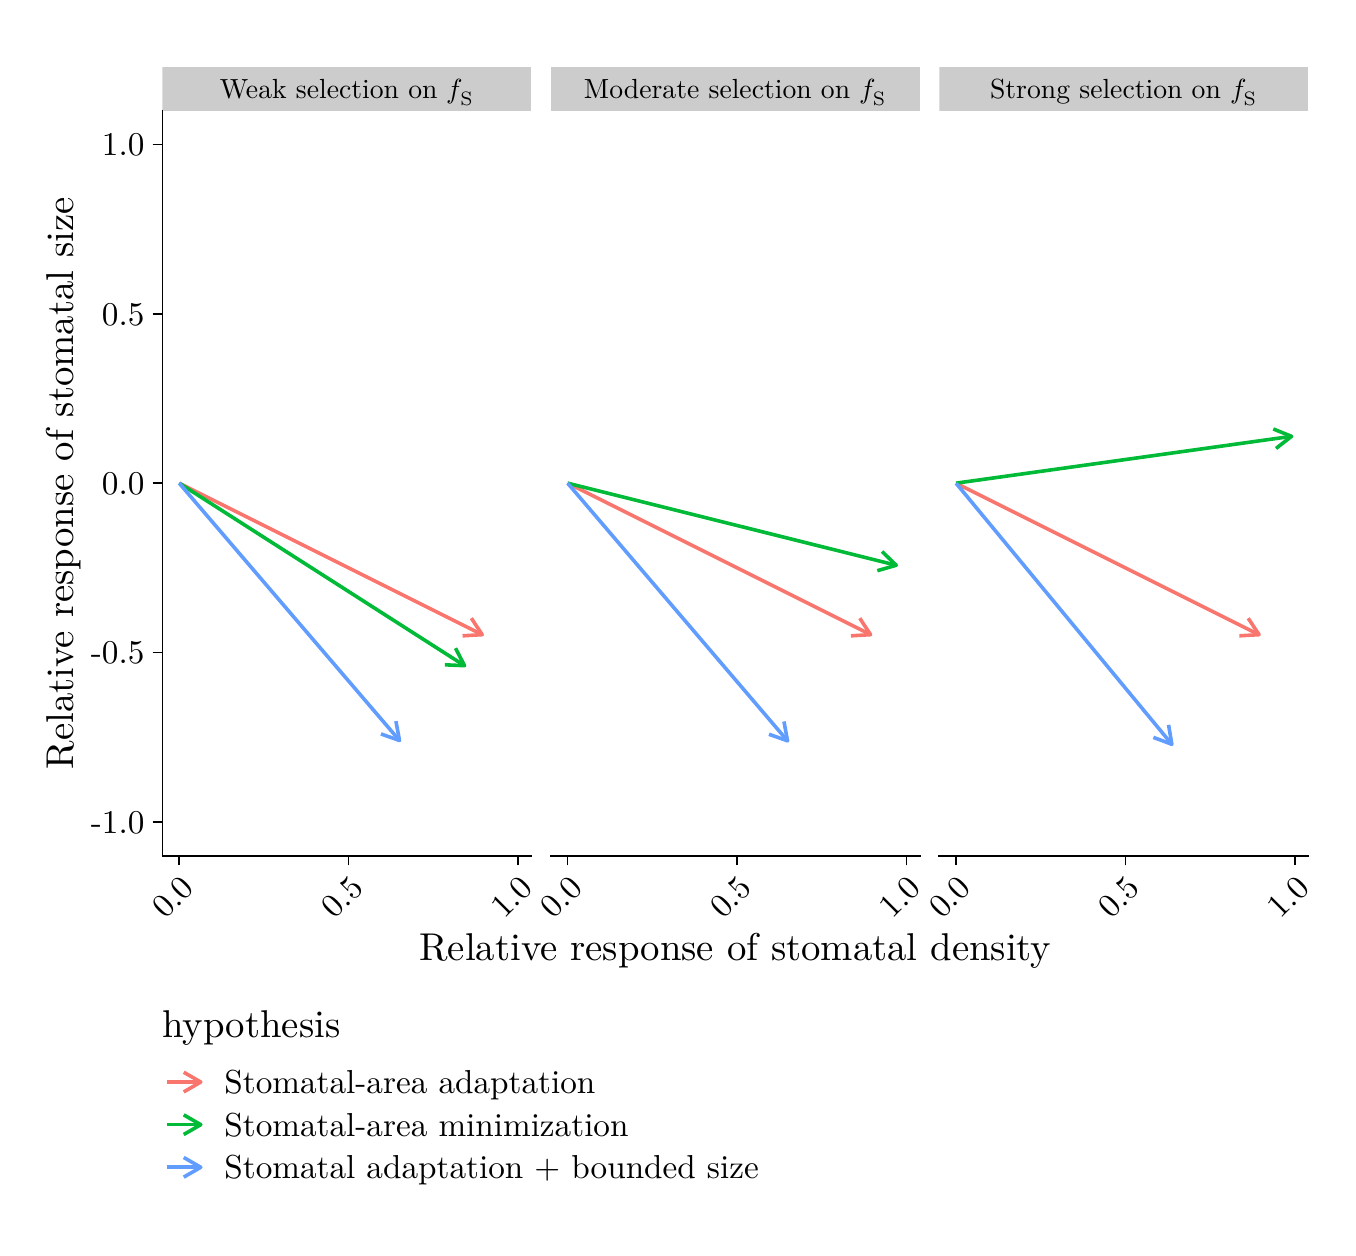
\begin{tikzpicture}[x=1pt,y=1pt]
\definecolor{fillColor}{RGB}{255,255,255}
\path[use as bounding box,fill=fillColor,fill opacity=0.00] (0,0) rectangle (469.75,433.62);
\begin{scope}
\path[clip] ( 48.69,134.38) rectangle (182.05,403.67);
\definecolor{drawColor}{RGB}{248,118,109}

\path[draw=drawColor,line width= 1.3pt,line join=round] ( 54.75,269.02) -- (164.24,214.28);

\path[draw=drawColor,line width= 1.3pt,line join=round] (157.14,213.86) --
	(164.24,214.28) --
	(160.32,220.22);
\definecolor{drawColor}{RGB}{0,186,56}

\path[draw=drawColor,line width= 1.3pt,line join=round] ( 54.75,269.02) -- (157.87,203.07);

\path[draw=drawColor,line width= 1.3pt,line join=round] (150.77,203.39) --
	(157.87,203.07) --
	(154.60,209.39);
\definecolor{drawColor}{RGB}{97,156,255}

\path[draw=drawColor,line width= 1.3pt,line join=round] ( 54.75,269.02) -- (134.36,176.04);

\path[draw=drawColor,line width= 1.3pt,line join=round] (127.65,178.41) --
	(134.36,176.04) --
	(133.06,183.03);
\end{scope}
\begin{scope}
\path[clip] (189.05,134.38) rectangle (322.40,403.67);
\definecolor{drawColor}{RGB}{248,118,109}

\path[draw=drawColor,line width= 1.3pt,line join=round] (195.11,269.02) -- (304.59,214.28);

\path[draw=drawColor,line width= 1.3pt,line join=round] (297.49,213.86) --
	(304.59,214.28) --
	(300.67,220.22);
\definecolor{drawColor}{RGB}{0,186,56}

\path[draw=drawColor,line width= 1.3pt,line join=round] (195.11,269.02) -- (313.86,239.36);

\path[draw=drawColor,line width= 1.3pt,line join=round] (307.02,237.40) --
	(313.86,239.36) --
	(308.75,244.30);
\definecolor{drawColor}{RGB}{97,156,255}

\path[draw=drawColor,line width= 1.3pt,line join=round] (195.11,269.02) -- (274.57,175.92);

\path[draw=drawColor,line width= 1.3pt,line join=round] (267.87,178.29) --
	(274.57,175.92) --
	(273.28,182.91);
\end{scope}
\begin{scope}
\path[clip] (329.40,134.38) rectangle (462.76,403.67);
\definecolor{drawColor}{RGB}{248,118,109}

\path[draw=drawColor,line width= 1.3pt,line join=round] (335.46,269.02) -- (444.95,214.28);

\path[draw=drawColor,line width= 1.3pt,line join=round] (437.84,213.86) --
	(444.95,214.28) --
	(441.03,220.22);
\definecolor{drawColor}{RGB}{0,186,56}

\path[draw=drawColor,line width= 1.3pt,line join=round] (335.46,269.02) -- (456.69,285.94);

\path[draw=drawColor,line width= 1.3pt,line join=round] (451.08,281.57) --
	(456.69,285.94) --
	(450.10,288.61);
\definecolor{drawColor}{RGB}{97,156,255}

\path[draw=drawColor,line width= 1.3pt,line join=round] (335.46,269.02) -- (413.44,174.67);

\path[draw=drawColor,line width= 1.3pt,line join=round] (406.78,177.16) --
	(413.44,174.67) --
	(412.26,181.69);
\end{scope}
\begin{scope}
\path[clip] ( 48.69,403.67) rectangle (182.05,419.50);
\definecolor{fillColor}{gray}{0.80}

\path[fill=fillColor] ( 48.69,403.67) rectangle (182.05,419.50);
\definecolor{drawColor}{RGB}{0,0,0}

\node[text=drawColor,anchor=base,inner sep=0pt, outer sep=0pt, scale=  1.00] at (115.37,408.14) {Weak selection on $f_\textrm{S}$};
\end{scope}
\begin{scope}
\path[clip] (189.05,403.67) rectangle (322.40,419.50);
\definecolor{fillColor}{gray}{0.80}

\path[fill=fillColor] (189.05,403.67) rectangle (322.40,419.50);
\definecolor{drawColor}{RGB}{0,0,0}

\node[text=drawColor,anchor=base,inner sep=0pt, outer sep=0pt, scale=  1.00] at (255.72,408.14) {Moderate selection on $f_\textrm{S}$};
\end{scope}
\begin{scope}
\path[clip] (329.40,403.67) rectangle (462.76,419.50);
\definecolor{fillColor}{gray}{0.80}

\path[fill=fillColor] (329.40,403.67) rectangle (462.75,419.50);
\definecolor{drawColor}{RGB}{0,0,0}

\node[text=drawColor,anchor=base,inner sep=0pt, outer sep=0pt, scale=  1.00] at (396.08,408.14) {Strong selection on $f_\textrm{S}$};
\end{scope}
\begin{scope}
\path[clip] (  0.00,  0.00) rectangle (469.75,433.62);
\definecolor{drawColor}{RGB}{0,0,0}

\path[draw=drawColor,line width= 0.6pt,line join=round,line cap=rect] ( 48.69,134.38) --
	(182.05,134.38);
\end{scope}
\begin{scope}
\path[clip] (  0.00,  0.00) rectangle (469.75,433.62);
\definecolor{drawColor}{RGB}{0,0,0}

\path[draw=drawColor,line width= 0.6pt,line join=round] ( 54.75,130.88) --
	( 54.75,134.38);

\path[draw=drawColor,line width= 0.6pt,line join=round] (115.96,130.88) --
	(115.96,134.38);

\path[draw=drawColor,line width= 0.6pt,line join=round] (177.16,130.88) --
	(177.16,134.38);
\end{scope}
\begin{scope}
\path[clip] (  0.00,  0.00) rectangle (469.75,433.62);
\definecolor{drawColor}{RGB}{0,0,0}

\node[text=drawColor,rotate= 45.00,anchor=base east,inner sep=0pt, outer sep=0pt, scale=  1.20] at ( 60.60,122.03) {0.0};

\node[text=drawColor,rotate= 45.00,anchor=base east,inner sep=0pt, outer sep=0pt, scale=  1.20] at (121.80,122.03) {0.5};

\node[text=drawColor,rotate= 45.00,anchor=base east,inner sep=0pt, outer sep=0pt, scale=  1.20] at (183.00,122.03) {1.0};
\end{scope}
\begin{scope}
\path[clip] (  0.00,  0.00) rectangle (469.75,433.62);
\definecolor{drawColor}{RGB}{0,0,0}

\path[draw=drawColor,line width= 0.6pt,line join=round,line cap=rect] (189.05,134.38) --
	(322.40,134.38);
\end{scope}
\begin{scope}
\path[clip] (  0.00,  0.00) rectangle (469.75,433.62);
\definecolor{drawColor}{RGB}{0,0,0}

\path[draw=drawColor,line width= 0.6pt,line join=round] (195.11,130.88) --
	(195.11,134.38);

\path[draw=drawColor,line width= 0.6pt,line join=round] (256.31,130.88) --
	(256.31,134.38);

\path[draw=drawColor,line width= 0.6pt,line join=round] (317.51,130.88) --
	(317.51,134.38);
\end{scope}
\begin{scope}
\path[clip] (  0.00,  0.00) rectangle (469.75,433.62);
\definecolor{drawColor}{RGB}{0,0,0}

\node[text=drawColor,rotate= 45.00,anchor=base east,inner sep=0pt, outer sep=0pt, scale=  1.20] at (200.95,122.03) {0.0};

\node[text=drawColor,rotate= 45.00,anchor=base east,inner sep=0pt, outer sep=0pt, scale=  1.20] at (262.15,122.03) {0.5};

\node[text=drawColor,rotate= 45.00,anchor=base east,inner sep=0pt, outer sep=0pt, scale=  1.20] at (323.36,122.03) {1.0};
\end{scope}
\begin{scope}
\path[clip] (  0.00,  0.00) rectangle (469.75,433.62);
\definecolor{drawColor}{RGB}{0,0,0}

\path[draw=drawColor,line width= 0.6pt,line join=round,line cap=rect] (329.40,134.38) --
	(462.76,134.38);
\end{scope}
\begin{scope}
\path[clip] (  0.00,  0.00) rectangle (469.75,433.62);
\definecolor{drawColor}{RGB}{0,0,0}

\path[draw=drawColor,line width= 0.6pt,line join=round] (335.46,130.88) --
	(335.46,134.38);

\path[draw=drawColor,line width= 0.6pt,line join=round] (396.67,130.88) --
	(396.67,134.38);

\path[draw=drawColor,line width= 0.6pt,line join=round] (457.87,130.88) --
	(457.87,134.38);
\end{scope}
\begin{scope}
\path[clip] (  0.00,  0.00) rectangle (469.75,433.62);
\definecolor{drawColor}{RGB}{0,0,0}

\node[text=drawColor,rotate= 45.00,anchor=base east,inner sep=0pt, outer sep=0pt, scale=  1.20] at (341.31,122.03) {0.0};

\node[text=drawColor,rotate= 45.00,anchor=base east,inner sep=0pt, outer sep=0pt, scale=  1.20] at (402.51,122.03) {0.5};

\node[text=drawColor,rotate= 45.00,anchor=base east,inner sep=0pt, outer sep=0pt, scale=  1.20] at (463.71,122.03) {1.0};
\end{scope}
\begin{scope}
\path[clip] (  0.00,  0.00) rectangle (469.75,433.62);
\definecolor{drawColor}{RGB}{0,0,0}

\path[draw=drawColor,line width= 0.6pt,line join=round,line cap=rect] ( 48.69,134.38) --
	( 48.69,403.67);
\end{scope}
\begin{scope}
\path[clip] (  0.00,  0.00) rectangle (469.75,433.62);
\definecolor{drawColor}{RGB}{0,0,0}

\node[text=drawColor,anchor=base east,inner sep=0pt, outer sep=0pt, scale=  1.20] at ( 42.19,142.49) {-1.0};

\node[text=drawColor,anchor=base east,inner sep=0pt, outer sep=0pt, scale=  1.20] at ( 42.19,203.69) {-0.5};

\node[text=drawColor,anchor=base east,inner sep=0pt, outer sep=0pt, scale=  1.20] at ( 42.19,264.89) {0.0};

\node[text=drawColor,anchor=base east,inner sep=0pt, outer sep=0pt, scale=  1.20] at ( 42.19,326.10) {0.5};

\node[text=drawColor,anchor=base east,inner sep=0pt, outer sep=0pt, scale=  1.20] at ( 42.19,387.30) {1.0};
\end{scope}
\begin{scope}
\path[clip] (  0.00,  0.00) rectangle (469.75,433.62);
\definecolor{drawColor}{RGB}{0,0,0}

\path[draw=drawColor,line width= 0.6pt,line join=round] ( 45.19,146.62) --
	( 48.69,146.62);

\path[draw=drawColor,line width= 0.6pt,line join=round] ( 45.19,207.82) --
	( 48.69,207.82);

\path[draw=drawColor,line width= 0.6pt,line join=round] ( 45.19,269.02) --
	( 48.69,269.02);

\path[draw=drawColor,line width= 0.6pt,line join=round] ( 45.19,330.23) --
	( 48.69,330.23);

\path[draw=drawColor,line width= 0.6pt,line join=round] ( 45.19,391.43) --
	( 48.69,391.43);
\end{scope}
\begin{scope}
\path[clip] (  0.00,  0.00) rectangle (469.75,433.62);
\definecolor{drawColor}{RGB}{0,0,0}

\node[text=drawColor,anchor=base,inner sep=0pt, outer sep=0pt, scale=  1.40] at (255.72, 96.40) {Relative response of stomatal density};
\end{scope}
\begin{scope}
\path[clip] (  0.00,  0.00) rectangle (469.75,433.62);
\definecolor{drawColor}{RGB}{0,0,0}

\node[text=drawColor,rotate= 90.00,anchor=base,inner sep=0pt, outer sep=0pt, scale=  1.40] at ( 16.64,269.02) {Relative response of stomatal size};
\end{scope}
\begin{scope}
\path[clip] (  0.00,  0.00) rectangle (469.75,433.62);
\definecolor{drawColor}{RGB}{0,0,0}

\node[text=drawColor,anchor=base west,inner sep=0pt, outer sep=0pt, scale=  1.40] at ( 48.69, 68.68) {hypothesis};
\end{scope}
\begin{scope}
\path[clip] (  0.00,  0.00) rectangle (469.75,433.62);
\definecolor{drawColor}{RGB}{248,118,109}

\path[draw=drawColor,line width= 1.3pt,line join=round] ( 50.23, 52.62) -- ( 62.55, 52.62);

\path[draw=drawColor,line width= 1.3pt,line join=round] ( 56.39, 49.06) --
	( 62.55, 52.62) --
	( 56.39, 56.17);
\end{scope}
\begin{scope}
\path[clip] (  0.00,  0.00) rectangle (469.75,433.62);
\definecolor{drawColor}{RGB}{0,186,56}

\path[draw=drawColor,line width= 1.3pt,line join=round] ( 50.23, 37.22) -- ( 62.55, 37.22);

\path[draw=drawColor,line width= 1.3pt,line join=round] ( 56.39, 33.66) --
	( 62.55, 37.22) --
	( 56.39, 40.77);
\end{scope}
\begin{scope}
\path[clip] (  0.00,  0.00) rectangle (469.75,433.62);
\definecolor{drawColor}{RGB}{97,156,255}

\path[draw=drawColor,line width= 1.3pt,line join=round] ( 50.23, 21.82) -- ( 62.55, 21.82);

\path[draw=drawColor,line width= 1.3pt,line join=round] ( 56.39, 18.26) --
	( 62.55, 21.82) --
	( 56.39, 25.37);
\end{scope}
\begin{scope}
\path[clip] (  0.00,  0.00) rectangle (469.75,433.62);
\definecolor{drawColor}{RGB}{0,0,0}

\node[text=drawColor,anchor=base west,inner sep=0pt, outer sep=0pt, scale=  1.20] at ( 71.09, 48.49) {Stomatal-area adaptation};
\end{scope}
\begin{scope}
\path[clip] (  0.00,  0.00) rectangle (469.75,433.62);
\definecolor{drawColor}{RGB}{0,0,0}

\node[text=drawColor,anchor=base west,inner sep=0pt, outer sep=0pt, scale=  1.20] at ( 71.09, 33.09) {Stomatal-area minimization};
\end{scope}
\begin{scope}
\path[clip] (  0.00,  0.00) rectangle (469.75,433.62);
\definecolor{drawColor}{RGB}{0,0,0}

\node[text=drawColor,anchor=base west,inner sep=0pt, outer sep=0pt, scale=  1.20] at ( 71.09, 17.69) {Stomatal adaptation + bounded size};
\end{scope}
\end{tikzpicture}

\end{figure}

\newpage

\begin{figure}
\caption{Among-species trait (co)variances are not sensitive to mutational ratio at stationarity. Dashed lines are the theoretical expectations for the interspecific variance in stomatal density ($V_{d_\mathrm{S}}^*$), stomatal size ($V_{a_\mathrm{S}}^*$), anatomical maximum stomatal conductance ($V_{g_\mathrm{s,max}}^*$), and covariance between density and size ($V_{d_\mathrm{S},a_\mathrm{S}}^*$) at stationarity. The theoretical expectations differ between the hypotheses, $H_2$: stomatal-area minimization (upper panel) and $H_3$: stomatal adaptation + bounded size (lower panel). The points are estimated from simulations of an ensemble of 1000 over a range of mutational ratios ($M_{d_\mathrm{S}} / M_{a_\mathrm{S}}$), where a value of 1 corresponds to the baseline scenario. The solid line behind each points indicates the 95\% bootstrap confidence interval. All other parameters are set to their baseline value as described in the ``Baseline parameter values'' subsection.}
% Created by tikzDevice version 0.12.6 on 2025-08-19 18:35:36
% !TEX encoding = UTF-8 Unicode
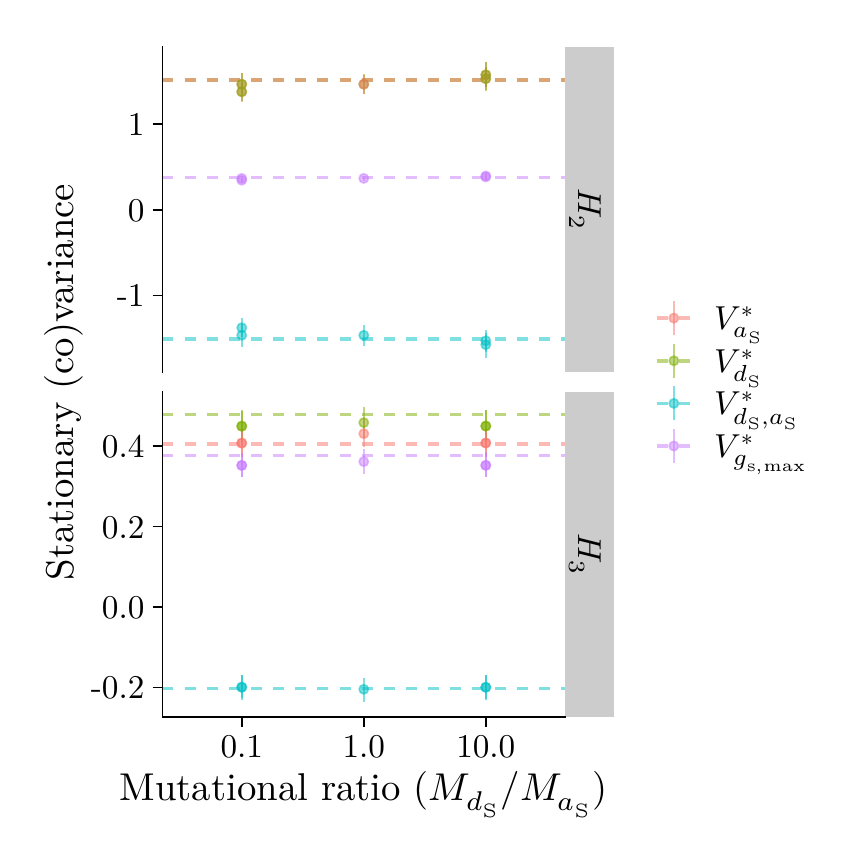
\begin{tikzpicture}[x=1pt,y=1pt]
\definecolor{fillColor}{RGB}{255,255,255}
\path[use as bounding box,fill=fillColor,fill opacity=0.00] (0,0) rectangle (289.08,289.08);
\begin{scope}
\path[clip] ( 48.69,164.52) rectangle (194.20,282.08);
\definecolor{drawColor}{RGB}{124,174,0}

\path[draw=drawColor,draw opacity=0.50,line width= 1.3pt,dash pattern=on 4pt off 4pt ,line join=round] ( 48.69,270.08) -- (194.20,270.08);
\definecolor{drawColor}{RGB}{248,118,109}

\path[draw=drawColor,draw opacity=0.50,line width= 1.3pt,dash pattern=on 4pt off 4pt ,line join=round] ( 48.69,270.08) -- (194.20,270.08);
\definecolor{drawColor}{RGB}{0,191,196}

\path[draw=drawColor,draw opacity=0.50,line width= 1.3pt,dash pattern=on 4pt off 4pt ,line join=round] ( 48.69,176.49) -- (194.20,176.49);
\definecolor{drawColor}{RGB}{199,124,255}

\path[draw=drawColor,draw opacity=0.50,line width= 1.3pt,dash pattern=on 4pt off 4pt ,line join=round] ( 48.69,234.98) -- (194.20,234.98);
\definecolor{drawColor}{RGB}{248,118,109}

\path[draw=drawColor,draw opacity=0.50,line width= 0.7pt,line join=round] (165.54,267.51) -- (165.54,276.74);
\definecolor{drawColor}{RGB}{124,174,0}

\path[draw=drawColor,draw opacity=0.50,line width= 0.7pt,line join=round] (165.54,267.63) -- (165.54,276.60);
\definecolor{drawColor}{RGB}{0,191,196}

\path[draw=drawColor,draw opacity=0.50,line width= 0.7pt,line join=round] (165.54,169.86) -- (165.54,178.74);
\definecolor{drawColor}{RGB}{248,118,109}

\path[draw=drawColor,draw opacity=0.50,line width= 0.7pt,line join=round] (165.54,266.39) -- (165.54,274.89);
\definecolor{drawColor}{RGB}{124,174,0}

\path[draw=drawColor,draw opacity=0.50,line width= 0.7pt,line join=round] (165.54,266.37) -- (165.54,274.72);
\definecolor{drawColor}{RGB}{0,191,196}

\path[draw=drawColor,draw opacity=0.50,line width= 0.7pt,line join=round] ( 77.35,173.76) -- ( 77.35,181.84);

\path[draw=drawColor,draw opacity=0.50,line width= 0.7pt,line join=round] (165.54,171.96) -- (165.54,179.99);
\definecolor{drawColor}{RGB}{248,118,109}

\path[draw=drawColor,draw opacity=0.50,line width= 0.7pt,line join=round] ( 77.35,264.67) -- ( 77.35,272.66);
\definecolor{drawColor}{RGB}{124,174,0}

\path[draw=drawColor,draw opacity=0.50,line width= 0.7pt,line join=round] ( 77.35,264.93) -- ( 77.35,272.84);
\definecolor{drawColor}{RGB}{0,191,196}

\path[draw=drawColor,draw opacity=0.50,line width= 0.7pt,line join=round] (121.45,174.03) -- (121.45,181.49);
\definecolor{drawColor}{RGB}{248,118,109}

\path[draw=drawColor,draw opacity=0.50,line width= 0.7pt,line join=round] ( 77.35,262.14) -- ( 77.35,269.46);
\definecolor{drawColor}{RGB}{124,174,0}

\path[draw=drawColor,draw opacity=0.50,line width= 0.7pt,line join=round] (121.45,265.02) -- (121.45,272.24);
\definecolor{drawColor}{RGB}{248,118,109}

\path[draw=drawColor,draw opacity=0.50,line width= 0.7pt,line join=round] (121.45,265.17) -- (121.45,272.15);
\definecolor{drawColor}{RGB}{124,174,0}

\path[draw=drawColor,draw opacity=0.50,line width= 0.7pt,line join=round] ( 77.35,262.52) -- ( 77.35,269.37);
\definecolor{drawColor}{RGB}{0,191,196}

\path[draw=drawColor,draw opacity=0.50,line width= 0.7pt,line join=round] ( 77.35,177.41) -- ( 77.35,184.21);
\definecolor{drawColor}{RGB}{199,124,255}

\path[draw=drawColor,draw opacity=0.50,line width= 0.7pt,line join=round] (165.54,234.40) -- (165.54,236.69);

\path[draw=drawColor,draw opacity=0.50,line width= 0.7pt,line join=round] (165.54,234.16) -- (165.54,236.22);

\path[draw=drawColor,draw opacity=0.50,line width= 0.7pt,line join=round] ( 77.35,233.63) -- ( 77.35,235.65);

\path[draw=drawColor,draw opacity=0.50,line width= 0.7pt,line join=round] (121.45,233.72) -- (121.45,235.59);

\path[draw=drawColor,draw opacity=0.50,line width= 0.7pt,line join=round] ( 77.35,233.07) -- ( 77.35,234.76);
\definecolor{drawColor}{RGB}{248,118,109}
\definecolor{fillColor}{RGB}{248,118,109}

\path[draw=drawColor,draw opacity=0.50,line width= 0.6pt,line join=round,line cap=round,fill=fillColor,fill opacity=0.50] (165.54,272.04) circle (  1.69);
\definecolor{drawColor}{RGB}{124,174,0}
\definecolor{fillColor}{RGB}{124,174,0}

\path[draw=drawColor,draw opacity=0.50,line width= 0.6pt,line join=round,line cap=round,fill=fillColor,fill opacity=0.50] (165.54,272.05) circle (  1.69);
\definecolor{drawColor}{RGB}{0,191,196}
\definecolor{fillColor}{RGB}{0,191,196}

\path[draw=drawColor,draw opacity=0.50,line width= 0.6pt,line join=round,line cap=round,fill=fillColor,fill opacity=0.50] (165.54,174.53) circle (  1.69);
\definecolor{drawColor}{RGB}{248,118,109}
\definecolor{fillColor}{RGB}{248,118,109}

\path[draw=drawColor,draw opacity=0.50,line width= 0.6pt,line join=round,line cap=round,fill=fillColor,fill opacity=0.50] (165.54,270.62) circle (  1.69);
\definecolor{drawColor}{RGB}{124,174,0}
\definecolor{fillColor}{RGB}{124,174,0}

\path[draw=drawColor,draw opacity=0.50,line width= 0.6pt,line join=round,line cap=round,fill=fillColor,fill opacity=0.50] (165.54,270.66) circle (  1.69);
\definecolor{drawColor}{RGB}{0,191,196}
\definecolor{fillColor}{RGB}{0,191,196}

\path[draw=drawColor,draw opacity=0.50,line width= 0.6pt,line join=round,line cap=round,fill=fillColor,fill opacity=0.50] ( 77.35,177.93) circle (  1.69);

\path[draw=drawColor,draw opacity=0.50,line width= 0.6pt,line join=round,line cap=round,fill=fillColor,fill opacity=0.50] (165.54,175.93) circle (  1.69);
\definecolor{drawColor}{RGB}{248,118,109}
\definecolor{fillColor}{RGB}{248,118,109}

\path[draw=drawColor,draw opacity=0.50,line width= 0.6pt,line join=round,line cap=round,fill=fillColor,fill opacity=0.50] ( 77.35,268.65) circle (  1.69);
\definecolor{drawColor}{RGB}{124,174,0}
\definecolor{fillColor}{RGB}{124,174,0}

\path[draw=drawColor,draw opacity=0.50,line width= 0.6pt,line join=round,line cap=round,fill=fillColor,fill opacity=0.50] ( 77.35,268.64) circle (  1.69);
\definecolor{drawColor}{RGB}{0,191,196}
\definecolor{fillColor}{RGB}{0,191,196}

\path[draw=drawColor,draw opacity=0.50,line width= 0.6pt,line join=round,line cap=round,fill=fillColor,fill opacity=0.50] (121.45,177.92) circle (  1.69);
\definecolor{drawColor}{RGB}{248,118,109}
\definecolor{fillColor}{RGB}{248,118,109}

\path[draw=drawColor,draw opacity=0.50,line width= 0.6pt,line join=round,line cap=round,fill=fillColor,fill opacity=0.50] ( 77.35,265.93) circle (  1.69);
\definecolor{drawColor}{RGB}{124,174,0}
\definecolor{fillColor}{RGB}{124,174,0}

\path[draw=drawColor,draw opacity=0.50,line width= 0.6pt,line join=round,line cap=round,fill=fillColor,fill opacity=0.50] (121.45,268.64) circle (  1.69);
\definecolor{drawColor}{RGB}{248,118,109}
\definecolor{fillColor}{RGB}{248,118,109}

\path[draw=drawColor,draw opacity=0.50,line width= 0.6pt,line join=round,line cap=round,fill=fillColor,fill opacity=0.50] (121.45,268.66) circle (  1.69);
\definecolor{drawColor}{RGB}{124,174,0}
\definecolor{fillColor}{RGB}{124,174,0}

\path[draw=drawColor,draw opacity=0.50,line width= 0.6pt,line join=round,line cap=round,fill=fillColor,fill opacity=0.50] ( 77.35,265.92) circle (  1.69);
\definecolor{drawColor}{RGB}{0,191,196}
\definecolor{fillColor}{RGB}{0,191,196}

\path[draw=drawColor,draw opacity=0.50,line width= 0.6pt,line join=round,line cap=round,fill=fillColor,fill opacity=0.50] ( 77.35,180.65) circle (  1.69);
\definecolor{drawColor}{RGB}{199,124,255}
\definecolor{fillColor}{RGB}{199,124,255}

\path[draw=drawColor,draw opacity=0.50,line width= 0.6pt,line join=round,line cap=round,fill=fillColor,fill opacity=0.50] (165.54,235.48) circle (  1.69);

\path[draw=drawColor,draw opacity=0.50,line width= 0.6pt,line join=round,line cap=round,fill=fillColor,fill opacity=0.50] (165.54,235.14) circle (  1.69);

\path[draw=drawColor,draw opacity=0.50,line width= 0.6pt,line join=round,line cap=round,fill=fillColor,fill opacity=0.50] ( 77.35,234.62) circle (  1.69);

\path[draw=drawColor,draw opacity=0.50,line width= 0.6pt,line join=round,line cap=round,fill=fillColor,fill opacity=0.50] (121.45,234.62) circle (  1.69);

\path[draw=drawColor,draw opacity=0.50,line width= 0.6pt,line join=round,line cap=round,fill=fillColor,fill opacity=0.50] ( 77.35,233.95) circle (  1.69);
\end{scope}
\begin{scope}
\path[clip] ( 48.69, 39.96) rectangle (194.20,157.52);
\definecolor{drawColor}{RGB}{124,174,0}

\path[draw=drawColor,draw opacity=0.50,line width= 1.3pt,dash pattern=on 4pt off 4pt ,line join=round] ( 48.69,149.24) -- (194.20,149.24);
\definecolor{drawColor}{RGB}{248,118,109}

\path[draw=drawColor,draw opacity=0.50,line width= 1.3pt,dash pattern=on 4pt off 4pt ,line join=round] ( 48.69,138.54) -- (194.20,138.54);
\definecolor{drawColor}{RGB}{0,191,196}

\path[draw=drawColor,draw opacity=0.50,line width= 1.3pt,dash pattern=on 4pt off 4pt ,line join=round] ( 48.69, 50.35) -- (194.20, 50.35);
\definecolor{drawColor}{RGB}{199,124,255}

\path[draw=drawColor,draw opacity=0.50,line width= 1.3pt,dash pattern=on 4pt off 4pt ,line join=round] ( 48.69,134.54) -- (194.20,134.54);
\definecolor{drawColor}{RGB}{124,174,0}

\path[draw=drawColor,draw opacity=0.50,line width= 0.7pt,line join=round] (165.54,139.22) -- (165.54,150.96);

\path[draw=drawColor,draw opacity=0.50,line width= 0.7pt,line join=round] ( 77.35,139.24) -- ( 77.35,150.95);

\path[draw=drawColor,draw opacity=0.50,line width= 0.7pt,line join=round] ( 77.35,139.09) -- ( 77.35,150.69);

\path[draw=drawColor,draw opacity=0.50,line width= 0.7pt,line join=round] (121.45,140.92) -- (121.45,152.18);

\path[draw=drawColor,draw opacity=0.50,line width= 0.7pt,line join=round] (165.54,139.90) -- (165.54,150.99);
\definecolor{drawColor}{RGB}{248,118,109}

\path[draw=drawColor,draw opacity=0.50,line width= 0.7pt,line join=round] ( 77.35,134.07) -- ( 77.35,144.35);

\path[draw=drawColor,draw opacity=0.50,line width= 0.7pt,line join=round] (121.45,137.38) -- (121.45,147.62);

\path[draw=drawColor,draw opacity=0.50,line width= 0.7pt,line join=round] ( 77.35,133.79) -- ( 77.35,143.93);

\path[draw=drawColor,draw opacity=0.50,line width= 0.7pt,line join=round] (165.54,133.81) -- (165.54,143.89);

\path[draw=drawColor,draw opacity=0.50,line width= 0.7pt,line join=round] (165.54,133.98) -- (165.54,143.75);
\definecolor{drawColor}{RGB}{199,124,255}

\path[draw=drawColor,draw opacity=0.50,line width= 0.7pt,line join=round] (121.45,127.64) -- (121.45,136.85);
\definecolor{drawColor}{RGB}{0,191,196}

\path[draw=drawColor,draw opacity=0.50,line width= 0.7pt,line join=round] (165.54, 46.11) -- (165.54, 55.03);
\definecolor{drawColor}{RGB}{199,124,255}

\path[draw=drawColor,draw opacity=0.50,line width= 0.7pt,line join=round] (165.54,126.77) -- (165.54,135.68);
\definecolor{drawColor}{RGB}{0,191,196}

\path[draw=drawColor,draw opacity=0.50,line width= 0.7pt,line join=round] ( 77.35, 46.22) -- ( 77.35, 55.08);

\path[draw=drawColor,draw opacity=0.50,line width= 0.7pt,line join=round] (121.45, 45.30) -- (121.45, 54.09);
\definecolor{drawColor}{RGB}{199,124,255}

\path[draw=drawColor,draw opacity=0.50,line width= 0.7pt,line join=round] ( 77.35,126.72) -- ( 77.35,135.43);
\definecolor{drawColor}{RGB}{0,191,196}

\path[draw=drawColor,draw opacity=0.50,line width= 0.7pt,line join=round] (165.54, 46.44) -- (165.54, 55.03);
\definecolor{drawColor}{RGB}{199,124,255}

\path[draw=drawColor,draw opacity=0.50,line width= 0.7pt,line join=round] ( 77.35,126.59) -- ( 77.35,135.14);
\definecolor{drawColor}{RGB}{0,191,196}

\path[draw=drawColor,draw opacity=0.50,line width= 0.7pt,line join=round] ( 77.35, 46.77) -- ( 77.35, 55.28);
\definecolor{drawColor}{RGB}{199,124,255}

\path[draw=drawColor,draw opacity=0.50,line width= 0.7pt,line join=round] (165.54,126.81) -- (165.54,135.32);
\definecolor{drawColor}{RGB}{124,174,0}
\definecolor{fillColor}{RGB}{124,174,0}

\path[draw=drawColor,draw opacity=0.50,line width= 0.6pt,line join=round,line cap=round,fill=fillColor,fill opacity=0.50] (165.54,145.13) circle (  1.69);

\path[draw=drawColor,draw opacity=0.50,line width= 0.6pt,line join=round,line cap=round,fill=fillColor,fill opacity=0.50] ( 77.35,145.12) circle (  1.69);

\path[draw=drawColor,draw opacity=0.50,line width= 0.6pt,line join=round,line cap=round,fill=fillColor,fill opacity=0.50] ( 77.35,145.03) circle (  1.69);

\path[draw=drawColor,draw opacity=0.50,line width= 0.6pt,line join=round,line cap=round,fill=fillColor,fill opacity=0.50] (121.45,146.36) circle (  1.69);

\path[draw=drawColor,draw opacity=0.50,line width= 0.6pt,line join=round,line cap=round,fill=fillColor,fill opacity=0.50] (165.54,145.11) circle (  1.69);
\definecolor{drawColor}{RGB}{248,118,109}
\definecolor{fillColor}{RGB}{248,118,109}

\path[draw=drawColor,draw opacity=0.50,line width= 0.6pt,line join=round,line cap=round,fill=fillColor,fill opacity=0.50] ( 77.35,138.97) circle (  1.69);

\path[draw=drawColor,draw opacity=0.50,line width= 0.6pt,line join=round,line cap=round,fill=fillColor,fill opacity=0.50] (121.45,142.36) circle (  1.69);

\path[draw=drawColor,draw opacity=0.50,line width= 0.6pt,line join=round,line cap=round,fill=fillColor,fill opacity=0.50] ( 77.35,138.97) circle (  1.69);

\path[draw=drawColor,draw opacity=0.50,line width= 0.6pt,line join=round,line cap=round,fill=fillColor,fill opacity=0.50] (165.54,139.00) circle (  1.69);

\path[draw=drawColor,draw opacity=0.50,line width= 0.6pt,line join=round,line cap=round,fill=fillColor,fill opacity=0.50] (165.54,139.00) circle (  1.69);
\definecolor{drawColor}{RGB}{199,124,255}
\definecolor{fillColor}{RGB}{199,124,255}

\path[draw=drawColor,draw opacity=0.50,line width= 0.6pt,line join=round,line cap=round,fill=fillColor,fill opacity=0.50] (121.45,132.27) circle (  1.69);
\definecolor{drawColor}{RGB}{0,191,196}
\definecolor{fillColor}{RGB}{0,191,196}

\path[draw=drawColor,draw opacity=0.50,line width= 0.6pt,line join=round,line cap=round,fill=fillColor,fill opacity=0.50] (165.54, 50.73) circle (  1.69);
\definecolor{drawColor}{RGB}{199,124,255}
\definecolor{fillColor}{RGB}{199,124,255}

\path[draw=drawColor,draw opacity=0.50,line width= 0.6pt,line join=round,line cap=round,fill=fillColor,fill opacity=0.50] (165.54,130.93) circle (  1.69);
\definecolor{drawColor}{RGB}{0,191,196}
\definecolor{fillColor}{RGB}{0,191,196}

\path[draw=drawColor,draw opacity=0.50,line width= 0.6pt,line join=round,line cap=round,fill=fillColor,fill opacity=0.50] ( 77.35, 50.74) circle (  1.69);

\path[draw=drawColor,draw opacity=0.50,line width= 0.6pt,line join=round,line cap=round,fill=fillColor,fill opacity=0.50] (121.45, 50.01) circle (  1.69);
\definecolor{drawColor}{RGB}{199,124,255}
\definecolor{fillColor}{RGB}{199,124,255}

\path[draw=drawColor,draw opacity=0.50,line width= 0.6pt,line join=round,line cap=round,fill=fillColor,fill opacity=0.50] ( 77.35,130.93) circle (  1.69);
\definecolor{drawColor}{RGB}{0,191,196}
\definecolor{fillColor}{RGB}{0,191,196}

\path[draw=drawColor,draw opacity=0.50,line width= 0.6pt,line join=round,line cap=round,fill=fillColor,fill opacity=0.50] (165.54, 50.75) circle (  1.69);
\definecolor{drawColor}{RGB}{199,124,255}
\definecolor{fillColor}{RGB}{199,124,255}

\path[draw=drawColor,draw opacity=0.50,line width= 0.6pt,line join=round,line cap=round,fill=fillColor,fill opacity=0.50] ( 77.35,130.88) circle (  1.69);
\definecolor{drawColor}{RGB}{0,191,196}
\definecolor{fillColor}{RGB}{0,191,196}

\path[draw=drawColor,draw opacity=0.50,line width= 0.6pt,line join=round,line cap=round,fill=fillColor,fill opacity=0.50] ( 77.35, 50.79) circle (  1.69);
\definecolor{drawColor}{RGB}{199,124,255}
\definecolor{fillColor}{RGB}{199,124,255}

\path[draw=drawColor,draw opacity=0.50,line width= 0.6pt,line join=round,line cap=round,fill=fillColor,fill opacity=0.50] (165.54,130.93) circle (  1.69);
\end{scope}
\begin{scope}
\path[clip] (194.20,164.52) rectangle (211.80,282.08);
\definecolor{fillColor}{gray}{0.80}

\path[fill=fillColor] (194.20,164.52) rectangle (211.80,282.08);
\definecolor{drawColor}{RGB}{0,0,0}

\node[text=drawColor,rotate=-90.00,anchor=base,inner sep=0pt, outer sep=0pt, scale=  1.20] at (198.87,223.30) {$H_2$};
\end{scope}
\begin{scope}
\path[clip] (194.20, 39.96) rectangle (211.80,157.52);
\definecolor{fillColor}{gray}{0.80}

\path[fill=fillColor] (194.20, 39.96) rectangle (211.80,157.52);
\definecolor{drawColor}{RGB}{0,0,0}

\node[text=drawColor,rotate=-90.00,anchor=base,inner sep=0pt, outer sep=0pt, scale=  1.20] at (198.87, 98.74) {$H_3$};
\end{scope}
\begin{scope}
\path[clip] (  0.00,  0.00) rectangle (289.08,289.08);
\definecolor{drawColor}{RGB}{0,0,0}

\path[draw=drawColor,line width= 0.6pt,line join=round,line cap=rect] ( 48.69, 39.96) --
	(194.20, 39.96);
\end{scope}
\begin{scope}
\path[clip] (  0.00,  0.00) rectangle (289.08,289.08);
\definecolor{drawColor}{RGB}{0,0,0}

\path[draw=drawColor,line width= 0.6pt,line join=round] ( 77.35, 36.46) --
	( 77.35, 39.96);

\path[draw=drawColor,line width= 0.6pt,line join=round] (121.45, 36.46) --
	(121.45, 39.96);

\path[draw=drawColor,line width= 0.6pt,line join=round] (165.54, 36.46) --
	(165.54, 39.96);
\end{scope}
\begin{scope}
\path[clip] (  0.00,  0.00) rectangle (289.08,289.08);
\definecolor{drawColor}{RGB}{0,0,0}

\node[text=drawColor,anchor=base,inner sep=0pt, outer sep=0pt, scale=  1.20] at ( 77.35, 25.20) {0.1};

\node[text=drawColor,anchor=base,inner sep=0pt, outer sep=0pt, scale=  1.20] at (121.45, 25.20) {1.0};

\node[text=drawColor,anchor=base,inner sep=0pt, outer sep=0pt, scale=  1.20] at (165.54, 25.20) {10.0};
\end{scope}
\begin{scope}
\path[clip] (  0.00,  0.00) rectangle (289.08,289.08);
\definecolor{drawColor}{RGB}{0,0,0}

\path[draw=drawColor,line width= 0.6pt,line join=round,line cap=rect] ( 48.69,164.52) --
	( 48.69,282.08);
\end{scope}
\begin{scope}
\path[clip] (  0.00,  0.00) rectangle (289.08,289.08);
\definecolor{drawColor}{RGB}{0,0,0}

\node[text=drawColor,anchor=base east,inner sep=0pt, outer sep=0pt, scale=  1.20] at ( 42.19,188.15) {-1};

\node[text=drawColor,anchor=base east,inner sep=0pt, outer sep=0pt, scale=  1.20] at ( 42.19,219.15) {0};

\node[text=drawColor,anchor=base east,inner sep=0pt, outer sep=0pt, scale=  1.20] at ( 42.19,250.16) {1};
\end{scope}
\begin{scope}
\path[clip] (  0.00,  0.00) rectangle (289.08,289.08);
\definecolor{drawColor}{RGB}{0,0,0}

\path[draw=drawColor,line width= 0.6pt,line join=round] ( 45.19,192.28) --
	( 48.69,192.28);

\path[draw=drawColor,line width= 0.6pt,line join=round] ( 45.19,223.29) --
	( 48.69,223.29);

\path[draw=drawColor,line width= 0.6pt,line join=round] ( 45.19,254.29) --
	( 48.69,254.29);
\end{scope}
\begin{scope}
\path[clip] (  0.00,  0.00) rectangle (289.08,289.08);
\definecolor{drawColor}{RGB}{0,0,0}

\path[draw=drawColor,line width= 0.6pt,line join=round,line cap=rect] ( 48.69, 39.96) --
	( 48.69,157.52);
\end{scope}
\begin{scope}
\path[clip] (  0.00,  0.00) rectangle (289.08,289.08);
\definecolor{drawColor}{RGB}{0,0,0}

\node[text=drawColor,anchor=base east,inner sep=0pt, outer sep=0pt, scale=  1.20] at ( 42.19, 46.57) {-0.2};

\node[text=drawColor,anchor=base east,inner sep=0pt, outer sep=0pt, scale=  1.20] at ( 42.19, 75.61) {0.0};

\node[text=drawColor,anchor=base east,inner sep=0pt, outer sep=0pt, scale=  1.20] at ( 42.19,104.66) {0.2};

\node[text=drawColor,anchor=base east,inner sep=0pt, outer sep=0pt, scale=  1.20] at ( 42.19,133.71) {0.4};
\end{scope}
\begin{scope}
\path[clip] (  0.00,  0.00) rectangle (289.08,289.08);
\definecolor{drawColor}{RGB}{0,0,0}

\path[draw=drawColor,line width= 0.6pt,line join=round] ( 45.19, 50.70) --
	( 48.69, 50.70);

\path[draw=drawColor,line width= 0.6pt,line join=round] ( 45.19, 79.75) --
	( 48.69, 79.75);

\path[draw=drawColor,line width= 0.6pt,line join=round] ( 45.19,108.79) --
	( 48.69,108.79);

\path[draw=drawColor,line width= 0.6pt,line join=round] ( 45.19,137.84) --
	( 48.69,137.84);
\end{scope}
\begin{scope}
\path[clip] (  0.00,  0.00) rectangle (289.08,289.08);
\definecolor{drawColor}{RGB}{0,0,0}

\node[text=drawColor,anchor=base,inner sep=0pt, outer sep=0pt, scale=  1.40] at (121.45,  9.72) {Mutational ratio ($M_{d_\mathrm{S}} / M_{a_\mathrm{S}}$)};
\end{scope}
\begin{scope}
\path[clip] (  0.00,  0.00) rectangle (289.08,289.08);
\definecolor{drawColor}{RGB}{0,0,0}

\node[text=drawColor,rotate= 90.00,anchor=base,inner sep=0pt, outer sep=0pt, scale=  1.40] at ( 16.64,161.02) {Stationary (co)variance};
\end{scope}
\begin{scope}
\path[clip] (  0.00,  0.00) rectangle (289.08,289.08);
\definecolor{drawColor}{RGB}{248,118,109}

\path[draw=drawColor,draw opacity=0.50,line width= 1.3pt,dash pattern=on 4pt off 4pt ,line join=round] (227.34,184.12) -- (239.66,184.12);
\end{scope}
\begin{scope}
\path[clip] (  0.00,  0.00) rectangle (289.08,289.08);
\definecolor{drawColor}{RGB}{248,118,109}

\path[draw=drawColor,draw opacity=0.50,line width= 0.7pt,line join=round] (233.50,177.96) -- (233.50,190.28);
\definecolor{fillColor}{RGB}{248,118,109}

\path[draw=drawColor,draw opacity=0.50,line width= 0.6pt,line join=round,line cap=round,fill=fillColor,fill opacity=0.50] (233.50,184.12) circle (  1.69);
\end{scope}
\begin{scope}
\path[clip] (  0.00,  0.00) rectangle (289.08,289.08);
\definecolor{drawColor}{RGB}{124,174,0}

\path[draw=drawColor,draw opacity=0.50,line width= 1.3pt,dash pattern=on 4pt off 4pt ,line join=round] (227.34,168.72) -- (239.66,168.72);
\end{scope}
\begin{scope}
\path[clip] (  0.00,  0.00) rectangle (289.08,289.08);
\definecolor{drawColor}{RGB}{124,174,0}

\path[draw=drawColor,draw opacity=0.50,line width= 0.7pt,line join=round] (233.50,162.56) -- (233.50,174.88);
\definecolor{fillColor}{RGB}{124,174,0}

\path[draw=drawColor,draw opacity=0.50,line width= 0.6pt,line join=round,line cap=round,fill=fillColor,fill opacity=0.50] (233.50,168.72) circle (  1.69);
\end{scope}
\begin{scope}
\path[clip] (  0.00,  0.00) rectangle (289.08,289.08);
\definecolor{drawColor}{RGB}{0,191,196}

\path[draw=drawColor,draw opacity=0.50,line width= 1.3pt,dash pattern=on 4pt off 4pt ,line join=round] (227.34,153.32) -- (239.66,153.32);
\end{scope}
\begin{scope}
\path[clip] (  0.00,  0.00) rectangle (289.08,289.08);
\definecolor{drawColor}{RGB}{0,191,196}

\path[draw=drawColor,draw opacity=0.50,line width= 0.7pt,line join=round] (233.50,147.16) -- (233.50,159.48);
\definecolor{fillColor}{RGB}{0,191,196}

\path[draw=drawColor,draw opacity=0.50,line width= 0.6pt,line join=round,line cap=round,fill=fillColor,fill opacity=0.50] (233.50,153.32) circle (  1.69);
\end{scope}
\begin{scope}
\path[clip] (  0.00,  0.00) rectangle (289.08,289.08);
\definecolor{drawColor}{RGB}{199,124,255}

\path[draw=drawColor,draw opacity=0.50,line width= 1.3pt,dash pattern=on 4pt off 4pt ,line join=round] (227.34,137.92) -- (239.66,137.92);
\end{scope}
\begin{scope}
\path[clip] (  0.00,  0.00) rectangle (289.08,289.08);
\definecolor{drawColor}{RGB}{199,124,255}

\path[draw=drawColor,draw opacity=0.50,line width= 0.7pt,line join=round] (233.50,131.76) -- (233.50,144.08);
\definecolor{fillColor}{RGB}{199,124,255}

\path[draw=drawColor,draw opacity=0.50,line width= 0.6pt,line join=round,line cap=round,fill=fillColor,fill opacity=0.50] (233.50,137.92) circle (  1.69);
\end{scope}
\begin{scope}
\path[clip] (  0.00,  0.00) rectangle (289.08,289.08);
\definecolor{drawColor}{RGB}{0,0,0}

\node[text=drawColor,anchor=base west,inner sep=0pt, outer sep=0pt, scale=  1.20] at (248.20,179.99) {$V^*_{a_\mathrm{S}}$};
\end{scope}
\begin{scope}
\path[clip] (  0.00,  0.00) rectangle (289.08,289.08);
\definecolor{drawColor}{RGB}{0,0,0}

\node[text=drawColor,anchor=base west,inner sep=0pt, outer sep=0pt, scale=  1.20] at (248.20,164.59) {$V^*_{d_\mathrm{S}}$};
\end{scope}
\begin{scope}
\path[clip] (  0.00,  0.00) rectangle (289.08,289.08);
\definecolor{drawColor}{RGB}{0,0,0}

\node[text=drawColor,anchor=base west,inner sep=0pt, outer sep=0pt, scale=  1.20] at (248.20,149.19) {$V^*_{d_\mathrm{S},a_\mathrm{S}}$};
\end{scope}
\begin{scope}
\path[clip] (  0.00,  0.00) rectangle (289.08,289.08);
\definecolor{drawColor}{RGB}{0,0,0}

\node[text=drawColor,anchor=base west,inner sep=0pt, outer sep=0pt, scale=  1.20] at (248.20,133.79) {$V^*_{g_\mathrm{s,max}}$};
\end{scope}
\end{tikzpicture}

\end{figure}

\newpage

\begin{figure}
\caption{Among-species trait (co)variances are not sensitive to mutational correlation ($\rho_\mathrm{M}$) at stationarity. Dashed lines are the theoretical expectations for the interspecific variance in stomatal density ($V_{d_\mathrm{S}}^*$), stomatal size ($V_{a_\mathrm{S}}^*$), anatomical maximum stomatal conductance ($V_{g_\mathrm{s,max}}^*$), and covariance between density and size ($V_{d_\mathrm{S},a_\mathrm{S}}^*$) at stationarity. The theoretical expectations differ between the hypotheses, $H_2$: stomatal-area minimization (upper panel) and $H_3$: stomatal adaptation + bounded size (lower panel). The points are estimated from simulations of an ensemble of 1000 over a range of mutational correlations, where a value of 0 corresponds to the baseline scenario. The solid line behind each points indicates the 95\% bootstrap confidence interval. All other parameters are set to their baseline value as described in the ``Baseline parameter values'' subsection.}
% Created by tikzDevice version 0.12.6 on 2025-08-19 18:36:04
% !TEX encoding = UTF-8 Unicode
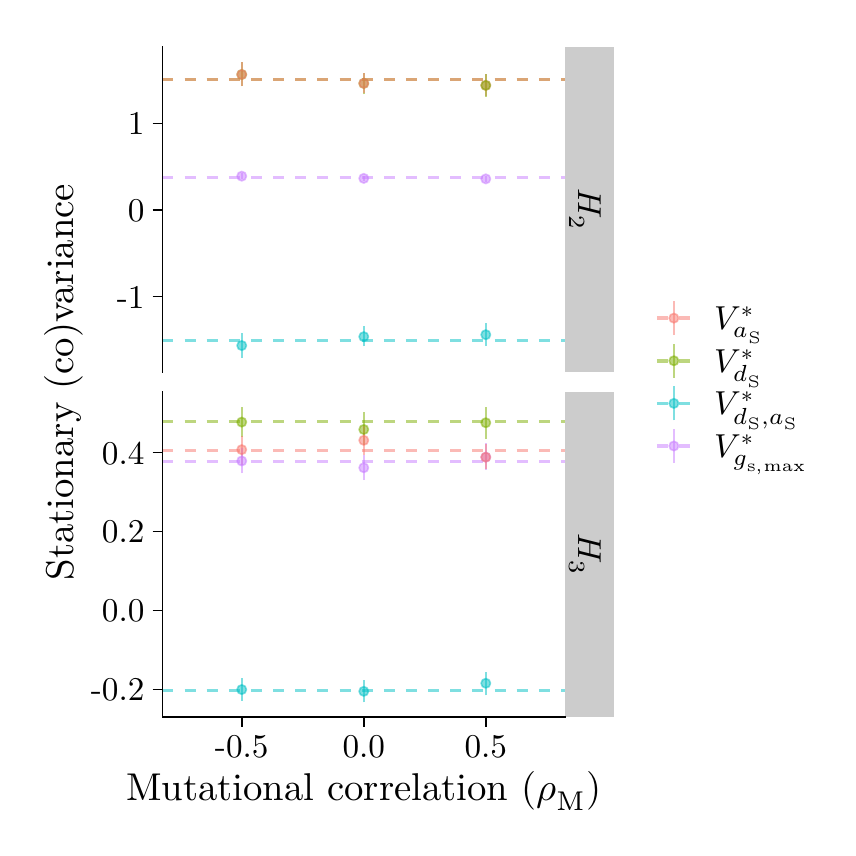
\begin{tikzpicture}[x=1pt,y=1pt]
\definecolor{fillColor}{RGB}{255,255,255}
\path[use as bounding box,fill=fillColor,fill opacity=0.00] (0,0) rectangle (289.08,289.08);
\begin{scope}
\path[clip] ( 48.69,164.52) rectangle (194.20,282.08);
\definecolor{drawColor}{RGB}{124,174,0}

\path[draw=drawColor,draw opacity=0.50,line width= 1.3pt,dash pattern=on 4pt off 4pt ,line join=round] ( 48.69,270.39) -- (194.20,270.39);
\definecolor{drawColor}{RGB}{248,118,109}

\path[draw=drawColor,draw opacity=0.50,line width= 1.3pt,dash pattern=on 4pt off 4pt ,line join=round] ( 48.69,270.39) -- (194.20,270.39);
\definecolor{drawColor}{RGB}{0,191,196}

\path[draw=drawColor,draw opacity=0.50,line width= 1.3pt,dash pattern=on 4pt off 4pt ,line join=round] ( 48.69,175.98) -- (194.20,175.98);
\definecolor{drawColor}{RGB}{199,124,255}

\path[draw=drawColor,draw opacity=0.50,line width= 1.3pt,dash pattern=on 4pt off 4pt ,line join=round] ( 48.69,234.98) -- (194.20,234.98);
\definecolor{drawColor}{RGB}{0,191,196}

\path[draw=drawColor,draw opacity=0.50,line width= 0.7pt,line join=round] ( 77.35,169.86) -- ( 77.35,178.75);
\definecolor{drawColor}{RGB}{124,174,0}

\path[draw=drawColor,draw opacity=0.50,line width= 0.7pt,line join=round] ( 77.35,267.87) -- ( 77.35,276.67);
\definecolor{drawColor}{RGB}{248,118,109}

\path[draw=drawColor,draw opacity=0.50,line width= 0.7pt,line join=round] ( 77.35,267.99) -- ( 77.35,276.74);
\definecolor{drawColor}{RGB}{0,191,196}

\path[draw=drawColor,draw opacity=0.50,line width= 0.7pt,line join=round] (165.54,174.04) -- (165.54,182.46);
\definecolor{drawColor}{RGB}{248,118,109}

\path[draw=drawColor,draw opacity=0.50,line width= 0.7pt,line join=round] (165.54,264.25) -- (165.54,272.45);
\definecolor{drawColor}{RGB}{124,174,0}

\path[draw=drawColor,draw opacity=0.50,line width= 0.7pt,line join=round] (165.54,264.16) -- (165.54,272.18);

\path[draw=drawColor,draw opacity=0.50,line width= 0.7pt,line join=round] (121.45,264.99) -- (121.45,272.62);
\definecolor{drawColor}{RGB}{248,118,109}

\path[draw=drawColor,draw opacity=0.50,line width= 0.7pt,line join=round] (121.45,265.31) -- (121.45,272.62);
\definecolor{drawColor}{RGB}{0,191,196}

\path[draw=drawColor,draw opacity=0.50,line width= 0.7pt,line join=round] (121.45,173.93) -- (121.45,181.20);
\definecolor{drawColor}{RGB}{199,124,255}

\path[draw=drawColor,draw opacity=0.50,line width= 0.7pt,line join=round] ( 77.35,234.35) -- ( 77.35,236.51);

\path[draw=drawColor,draw opacity=0.50,line width= 0.7pt,line join=round] (165.54,233.47) -- (165.54,235.47);

\path[draw=drawColor,draw opacity=0.50,line width= 0.7pt,line join=round] (121.45,233.71) -- (121.45,235.50);
\definecolor{drawColor}{RGB}{0,191,196}
\definecolor{fillColor}{RGB}{0,191,196}

\path[draw=drawColor,draw opacity=0.50,line width= 0.6pt,line join=round,line cap=round,fill=fillColor,fill opacity=0.50] ( 77.35,174.21) circle (  1.69);
\definecolor{drawColor}{RGB}{124,174,0}
\definecolor{fillColor}{RGB}{124,174,0}

\path[draw=drawColor,draw opacity=0.50,line width= 0.6pt,line join=round,line cap=round,fill=fillColor,fill opacity=0.50] ( 77.35,272.15) circle (  1.69);
\definecolor{drawColor}{RGB}{248,118,109}
\definecolor{fillColor}{RGB}{248,118,109}

\path[draw=drawColor,draw opacity=0.50,line width= 0.6pt,line join=round,line cap=round,fill=fillColor,fill opacity=0.50] ( 77.35,272.16) circle (  1.69);
\definecolor{drawColor}{RGB}{0,191,196}
\definecolor{fillColor}{RGB}{0,191,196}

\path[draw=drawColor,draw opacity=0.50,line width= 0.6pt,line join=round,line cap=round,fill=fillColor,fill opacity=0.50] (165.54,178.14) circle (  1.69);
\definecolor{drawColor}{RGB}{248,118,109}
\definecolor{fillColor}{RGB}{248,118,109}

\path[draw=drawColor,draw opacity=0.50,line width= 0.6pt,line join=round,line cap=round,fill=fillColor,fill opacity=0.50] (165.54,268.24) circle (  1.69);
\definecolor{drawColor}{RGB}{124,174,0}
\definecolor{fillColor}{RGB}{124,174,0}

\path[draw=drawColor,draw opacity=0.50,line width= 0.6pt,line join=round,line cap=round,fill=fillColor,fill opacity=0.50] (165.54,268.22) circle (  1.69);

\path[draw=drawColor,draw opacity=0.50,line width= 0.6pt,line join=round,line cap=round,fill=fillColor,fill opacity=0.50] (121.45,268.94) circle (  1.69);
\definecolor{drawColor}{RGB}{248,118,109}
\definecolor{fillColor}{RGB}{248,118,109}

\path[draw=drawColor,draw opacity=0.50,line width= 0.6pt,line join=round,line cap=round,fill=fillColor,fill opacity=0.50] (121.45,268.95) circle (  1.69);
\definecolor{drawColor}{RGB}{0,191,196}
\definecolor{fillColor}{RGB}{0,191,196}

\path[draw=drawColor,draw opacity=0.50,line width= 0.6pt,line join=round,line cap=round,fill=fillColor,fill opacity=0.50] (121.45,177.42) circle (  1.69);
\definecolor{drawColor}{RGB}{199,124,255}
\definecolor{fillColor}{RGB}{199,124,255}

\path[draw=drawColor,draw opacity=0.50,line width= 0.6pt,line join=round,line cap=round,fill=fillColor,fill opacity=0.50] ( 77.35,235.42) circle (  1.69);

\path[draw=drawColor,draw opacity=0.50,line width= 0.6pt,line join=round,line cap=round,fill=fillColor,fill opacity=0.50] (165.54,234.44) circle (  1.69);

\path[draw=drawColor,draw opacity=0.50,line width= 0.6pt,line join=round,line cap=round,fill=fillColor,fill opacity=0.50] (121.45,234.62) circle (  1.69);
\end{scope}
\begin{scope}
\path[clip] ( 48.69, 39.96) rectangle (194.20,157.52);
\definecolor{drawColor}{RGB}{124,174,0}

\path[draw=drawColor,draw opacity=0.50,line width= 1.3pt,dash pattern=on 4pt off 4pt ,line join=round] ( 48.69,146.73) -- (194.20,146.73);
\definecolor{drawColor}{RGB}{248,118,109}

\path[draw=drawColor,draw opacity=0.50,line width= 1.3pt,dash pattern=on 4pt off 4pt ,line join=round] ( 48.69,136.22) -- (194.20,136.22);
\definecolor{drawColor}{RGB}{0,191,196}

\path[draw=drawColor,draw opacity=0.50,line width= 1.3pt,dash pattern=on 4pt off 4pt ,line join=round] ( 48.69, 49.61) -- (194.20, 49.61);
\definecolor{drawColor}{RGB}{199,124,255}

\path[draw=drawColor,draw opacity=0.50,line width= 1.3pt,dash pattern=on 4pt off 4pt ,line join=round] ( 48.69,132.29) -- (194.20,132.29);
\definecolor{drawColor}{RGB}{124,174,0}

\path[draw=drawColor,draw opacity=0.50,line width= 0.7pt,line join=round] (121.45,138.34) -- (121.45,150.22);

\path[draw=drawColor,draw opacity=0.50,line width= 0.7pt,line join=round] (165.54,140.39) -- (165.54,151.95);

\path[draw=drawColor,draw opacity=0.50,line width= 0.7pt,line join=round] ( 77.35,141.33) -- ( 77.35,152.18);
\definecolor{drawColor}{RGB}{248,118,109}

\path[draw=drawColor,draw opacity=0.50,line width= 0.7pt,line join=round] ( 77.35,131.12) -- ( 77.35,141.65);

\path[draw=drawColor,draw opacity=0.50,line width= 0.7pt,line join=round] (121.45,134.82) -- (121.45,145.18);
\definecolor{drawColor}{RGB}{199,124,255}

\path[draw=drawColor,draw opacity=0.50,line width= 0.7pt,line join=round] (165.54,129.21) -- (165.54,138.93);

\path[draw=drawColor,draw opacity=0.50,line width= 0.7pt,line join=round] ( 77.35,127.98) -- ( 77.35,137.20);
\definecolor{drawColor}{RGB}{248,118,109}

\path[draw=drawColor,draw opacity=0.50,line width= 0.7pt,line join=round] (165.54,129.49) -- (165.54,138.67);
\definecolor{drawColor}{RGB}{199,124,255}

\path[draw=drawColor,draw opacity=0.50,line width= 0.7pt,line join=round] (121.45,125.57) -- (121.45,134.61);
\definecolor{drawColor}{RGB}{0,191,196}

\path[draw=drawColor,draw opacity=0.50,line width= 0.7pt,line join=round] (165.54, 47.82) -- (165.54, 56.43);

\path[draw=drawColor,draw opacity=0.50,line width= 0.7pt,line join=round] ( 77.35, 45.86) -- ( 77.35, 53.98);

\path[draw=drawColor,draw opacity=0.50,line width= 0.7pt,line join=round] (121.45, 45.30) -- (121.45, 53.22);
\definecolor{drawColor}{RGB}{124,174,0}
\definecolor{fillColor}{RGB}{124,174,0}

\path[draw=drawColor,draw opacity=0.50,line width= 0.6pt,line join=round,line cap=round,fill=fillColor,fill opacity=0.50] (121.45,143.89) circle (  1.69);

\path[draw=drawColor,draw opacity=0.50,line width= 0.6pt,line join=round,line cap=round,fill=fillColor,fill opacity=0.50] (165.54,146.32) circle (  1.69);

\path[draw=drawColor,draw opacity=0.50,line width= 0.6pt,line join=round,line cap=round,fill=fillColor,fill opacity=0.50] ( 77.35,146.55) circle (  1.69);
\definecolor{drawColor}{RGB}{248,118,109}
\definecolor{fillColor}{RGB}{248,118,109}

\path[draw=drawColor,draw opacity=0.50,line width= 0.6pt,line join=round,line cap=round,fill=fillColor,fill opacity=0.50] ( 77.35,136.60) circle (  1.69);

\path[draw=drawColor,draw opacity=0.50,line width= 0.6pt,line join=round,line cap=round,fill=fillColor,fill opacity=0.50] (121.45,139.97) circle (  1.69);
\definecolor{drawColor}{RGB}{199,124,255}
\definecolor{fillColor}{RGB}{199,124,255}

\path[draw=drawColor,draw opacity=0.50,line width= 0.6pt,line join=round,line cap=round,fill=fillColor,fill opacity=0.50] (165.54,133.88) circle (  1.69);

\path[draw=drawColor,draw opacity=0.50,line width= 0.6pt,line join=round,line cap=round,fill=fillColor,fill opacity=0.50] ( 77.35,132.51) circle (  1.69);
\definecolor{drawColor}{RGB}{248,118,109}
\definecolor{fillColor}{RGB}{248,118,109}

\path[draw=drawColor,draw opacity=0.50,line width= 0.6pt,line join=round,line cap=round,fill=fillColor,fill opacity=0.50] (165.54,133.88) circle (  1.69);
\definecolor{drawColor}{RGB}{199,124,255}
\definecolor{fillColor}{RGB}{199,124,255}

\path[draw=drawColor,draw opacity=0.50,line width= 0.6pt,line join=round,line cap=round,fill=fillColor,fill opacity=0.50] (121.45,130.06) circle (  1.69);
\definecolor{drawColor}{RGB}{0,191,196}
\definecolor{fillColor}{RGB}{0,191,196}

\path[draw=drawColor,draw opacity=0.50,line width= 0.6pt,line join=round,line cap=round,fill=fillColor,fill opacity=0.50] (165.54, 52.18) circle (  1.69);

\path[draw=drawColor,draw opacity=0.50,line width= 0.6pt,line join=round,line cap=round,fill=fillColor,fill opacity=0.50] ( 77.35, 49.91) circle (  1.69);

\path[draw=drawColor,draw opacity=0.50,line width= 0.6pt,line join=round,line cap=round,fill=fillColor,fill opacity=0.50] (121.45, 49.27) circle (  1.69);
\end{scope}
\begin{scope}
\path[clip] (194.20,164.52) rectangle (211.80,282.08);
\definecolor{fillColor}{gray}{0.80}

\path[fill=fillColor] (194.20,164.52) rectangle (211.80,282.08);
\definecolor{drawColor}{RGB}{0,0,0}

\node[text=drawColor,rotate=-90.00,anchor=base,inner sep=0pt, outer sep=0pt, scale=  1.20] at (198.87,223.30) {$H_2$};
\end{scope}
\begin{scope}
\path[clip] (194.20, 39.96) rectangle (211.80,157.52);
\definecolor{fillColor}{gray}{0.80}

\path[fill=fillColor] (194.20, 39.96) rectangle (211.80,157.52);
\definecolor{drawColor}{RGB}{0,0,0}

\node[text=drawColor,rotate=-90.00,anchor=base,inner sep=0pt, outer sep=0pt, scale=  1.20] at (198.87, 98.74) {$H_3$};
\end{scope}
\begin{scope}
\path[clip] (  0.00,  0.00) rectangle (289.08,289.08);
\definecolor{drawColor}{RGB}{0,0,0}

\path[draw=drawColor,line width= 0.6pt,line join=round,line cap=rect] ( 48.69, 39.96) --
	(194.20, 39.96);
\end{scope}
\begin{scope}
\path[clip] (  0.00,  0.00) rectangle (289.08,289.08);
\definecolor{drawColor}{RGB}{0,0,0}

\path[draw=drawColor,line width= 0.6pt,line join=round] ( 77.35, 36.46) --
	( 77.35, 39.96);

\path[draw=drawColor,line width= 0.6pt,line join=round] (121.45, 36.46) --
	(121.45, 39.96);

\path[draw=drawColor,line width= 0.6pt,line join=round] (165.54, 36.46) --
	(165.54, 39.96);
\end{scope}
\begin{scope}
\path[clip] (  0.00,  0.00) rectangle (289.08,289.08);
\definecolor{drawColor}{RGB}{0,0,0}

\node[text=drawColor,anchor=base,inner sep=0pt, outer sep=0pt, scale=  1.20] at ( 77.35, 25.20) {-0.5};

\node[text=drawColor,anchor=base,inner sep=0pt, outer sep=0pt, scale=  1.20] at (121.45, 25.20) {0.0};

\node[text=drawColor,anchor=base,inner sep=0pt, outer sep=0pt, scale=  1.20] at (165.54, 25.20) {0.5};
\end{scope}
\begin{scope}
\path[clip] (  0.00,  0.00) rectangle (289.08,289.08);
\definecolor{drawColor}{RGB}{0,0,0}

\path[draw=drawColor,line width= 0.6pt,line join=round,line cap=rect] ( 48.69,164.52) --
	( 48.69,282.08);
\end{scope}
\begin{scope}
\path[clip] (  0.00,  0.00) rectangle (289.08,289.08);
\definecolor{drawColor}{RGB}{0,0,0}

\node[text=drawColor,anchor=base east,inner sep=0pt, outer sep=0pt, scale=  1.20] at ( 42.19,187.77) {-1};

\node[text=drawColor,anchor=base east,inner sep=0pt, outer sep=0pt, scale=  1.20] at ( 42.19,219.05) {0};

\node[text=drawColor,anchor=base east,inner sep=0pt, outer sep=0pt, scale=  1.20] at ( 42.19,250.33) {1};
\end{scope}
\begin{scope}
\path[clip] (  0.00,  0.00) rectangle (289.08,289.08);
\definecolor{drawColor}{RGB}{0,0,0}

\path[draw=drawColor,line width= 0.6pt,line join=round] ( 45.19,191.90) --
	( 48.69,191.90);

\path[draw=drawColor,line width= 0.6pt,line join=round] ( 45.19,223.18) --
	( 48.69,223.18);

\path[draw=drawColor,line width= 0.6pt,line join=round] ( 45.19,254.46) --
	( 48.69,254.46);
\end{scope}
\begin{scope}
\path[clip] (  0.00,  0.00) rectangle (289.08,289.08);
\definecolor{drawColor}{RGB}{0,0,0}

\path[draw=drawColor,line width= 0.6pt,line join=round,line cap=rect] ( 48.69, 39.96) --
	( 48.69,157.52);
\end{scope}
\begin{scope}
\path[clip] (  0.00,  0.00) rectangle (289.08,289.08);
\definecolor{drawColor}{RGB}{0,0,0}

\node[text=drawColor,anchor=base east,inner sep=0pt, outer sep=0pt, scale=  1.20] at ( 42.19, 45.82) {-0.2};

\node[text=drawColor,anchor=base east,inner sep=0pt, outer sep=0pt, scale=  1.20] at ( 42.19, 74.35) {0.0};

\node[text=drawColor,anchor=base east,inner sep=0pt, outer sep=0pt, scale=  1.20] at ( 42.19,102.87) {0.2};

\node[text=drawColor,anchor=base east,inner sep=0pt, outer sep=0pt, scale=  1.20] at ( 42.19,131.40) {0.4};
\end{scope}
\begin{scope}
\path[clip] (  0.00,  0.00) rectangle (289.08,289.08);
\definecolor{drawColor}{RGB}{0,0,0}

\path[draw=drawColor,line width= 0.6pt,line join=round] ( 45.19, 49.95) --
	( 48.69, 49.95);

\path[draw=drawColor,line width= 0.6pt,line join=round] ( 45.19, 78.48) --
	( 48.69, 78.48);

\path[draw=drawColor,line width= 0.6pt,line join=round] ( 45.19,107.00) --
	( 48.69,107.00);

\path[draw=drawColor,line width= 0.6pt,line join=round] ( 45.19,135.53) --
	( 48.69,135.53);
\end{scope}
\begin{scope}
\path[clip] (  0.00,  0.00) rectangle (289.08,289.08);
\definecolor{drawColor}{RGB}{0,0,0}

\node[text=drawColor,anchor=base,inner sep=0pt, outer sep=0pt, scale=  1.40] at (121.45,  9.72) {Mutational correlation ($\rho_\mathrm{M}$)};
\end{scope}
\begin{scope}
\path[clip] (  0.00,  0.00) rectangle (289.08,289.08);
\definecolor{drawColor}{RGB}{0,0,0}

\node[text=drawColor,rotate= 90.00,anchor=base,inner sep=0pt, outer sep=0pt, scale=  1.40] at ( 16.64,161.02) {Stationary (co)variance};
\end{scope}
\begin{scope}
\path[clip] (  0.00,  0.00) rectangle (289.08,289.08);
\definecolor{drawColor}{RGB}{248,118,109}

\path[draw=drawColor,draw opacity=0.50,line width= 1.3pt,dash pattern=on 4pt off 4pt ,line join=round] (227.34,184.12) -- (239.66,184.12);
\end{scope}
\begin{scope}
\path[clip] (  0.00,  0.00) rectangle (289.08,289.08);
\definecolor{drawColor}{RGB}{248,118,109}

\path[draw=drawColor,draw opacity=0.50,line width= 0.7pt,line join=round] (233.50,177.96) -- (233.50,190.28);
\definecolor{fillColor}{RGB}{248,118,109}

\path[draw=drawColor,draw opacity=0.50,line width= 0.6pt,line join=round,line cap=round,fill=fillColor,fill opacity=0.50] (233.50,184.12) circle (  1.69);
\end{scope}
\begin{scope}
\path[clip] (  0.00,  0.00) rectangle (289.08,289.08);
\definecolor{drawColor}{RGB}{124,174,0}

\path[draw=drawColor,draw opacity=0.50,line width= 1.3pt,dash pattern=on 4pt off 4pt ,line join=round] (227.34,168.72) -- (239.66,168.72);
\end{scope}
\begin{scope}
\path[clip] (  0.00,  0.00) rectangle (289.08,289.08);
\definecolor{drawColor}{RGB}{124,174,0}

\path[draw=drawColor,draw opacity=0.50,line width= 0.7pt,line join=round] (233.50,162.56) -- (233.50,174.88);
\definecolor{fillColor}{RGB}{124,174,0}

\path[draw=drawColor,draw opacity=0.50,line width= 0.6pt,line join=round,line cap=round,fill=fillColor,fill opacity=0.50] (233.50,168.72) circle (  1.69);
\end{scope}
\begin{scope}
\path[clip] (  0.00,  0.00) rectangle (289.08,289.08);
\definecolor{drawColor}{RGB}{0,191,196}

\path[draw=drawColor,draw opacity=0.50,line width= 1.3pt,dash pattern=on 4pt off 4pt ,line join=round] (227.34,153.32) -- (239.66,153.32);
\end{scope}
\begin{scope}
\path[clip] (  0.00,  0.00) rectangle (289.08,289.08);
\definecolor{drawColor}{RGB}{0,191,196}

\path[draw=drawColor,draw opacity=0.50,line width= 0.7pt,line join=round] (233.50,147.16) -- (233.50,159.48);
\definecolor{fillColor}{RGB}{0,191,196}

\path[draw=drawColor,draw opacity=0.50,line width= 0.6pt,line join=round,line cap=round,fill=fillColor,fill opacity=0.50] (233.50,153.32) circle (  1.69);
\end{scope}
\begin{scope}
\path[clip] (  0.00,  0.00) rectangle (289.08,289.08);
\definecolor{drawColor}{RGB}{199,124,255}

\path[draw=drawColor,draw opacity=0.50,line width= 1.3pt,dash pattern=on 4pt off 4pt ,line join=round] (227.34,137.92) -- (239.66,137.92);
\end{scope}
\begin{scope}
\path[clip] (  0.00,  0.00) rectangle (289.08,289.08);
\definecolor{drawColor}{RGB}{199,124,255}

\path[draw=drawColor,draw opacity=0.50,line width= 0.7pt,line join=round] (233.50,131.76) -- (233.50,144.08);
\definecolor{fillColor}{RGB}{199,124,255}

\path[draw=drawColor,draw opacity=0.50,line width= 0.6pt,line join=round,line cap=round,fill=fillColor,fill opacity=0.50] (233.50,137.92) circle (  1.69);
\end{scope}
\begin{scope}
\path[clip] (  0.00,  0.00) rectangle (289.08,289.08);
\definecolor{drawColor}{RGB}{0,0,0}

\node[text=drawColor,anchor=base west,inner sep=0pt, outer sep=0pt, scale=  1.20] at (248.20,179.99) {$V^*_{a_\mathrm{S}}$};
\end{scope}
\begin{scope}
\path[clip] (  0.00,  0.00) rectangle (289.08,289.08);
\definecolor{drawColor}{RGB}{0,0,0}

\node[text=drawColor,anchor=base west,inner sep=0pt, outer sep=0pt, scale=  1.20] at (248.20,164.59) {$V^*_{d_\mathrm{S}}$};
\end{scope}
\begin{scope}
\path[clip] (  0.00,  0.00) rectangle (289.08,289.08);
\definecolor{drawColor}{RGB}{0,0,0}

\node[text=drawColor,anchor=base west,inner sep=0pt, outer sep=0pt, scale=  1.20] at (248.20,149.19) {$V^*_{d_\mathrm{S},a_\mathrm{S}}$};
\end{scope}
\begin{scope}
\path[clip] (  0.00,  0.00) rectangle (289.08,289.08);
\definecolor{drawColor}{RGB}{0,0,0}

\node[text=drawColor,anchor=base west,inner sep=0pt, outer sep=0pt, scale=  1.20] at (248.20,133.79) {$V^*_{g_\mathrm{s,max}}$};
\end{scope}
\end{tikzpicture}

\end{figure}

\newpage

\begin{figure}
\caption{Among-species trait (co)variances are not sensitive to the strength of selection on $g_\mathrm{s,max}$ at stationarity. Dashed lines are the theoretical expectations for the interspecific variance in stomatal density ($V_{d_\mathrm{S}}^*$), stomatal size ($V_{a_\mathrm{S}}^*$), anatomical maximum stomatal conductance ($V_{g_\mathrm{s,max}}^*$), and covariance between density and size ($V_{d_\mathrm{S},a_\mathrm{S}}^*$) at stationarity. The theoretical expectations differ between the hypotheses, $H_2$: stomatal-area minimization (upper panel) and $H_3$: stomatal adaptation + bounded size (lower panel). The points are estimated from simulations of an ensemble of 1000 over a range of selections strengths ($\omega$), where a value of 0.0377 corresponds to the baseline scenario. The solid line behind each points indicates the 95\% bootstrap confidence interval. All other parameters are set to their baseline value as described in the ``Baseline parameter values'' subsection.}
% Created by tikzDevice version 0.12.6 on 2025-08-19 18:36:07
% !TEX encoding = UTF-8 Unicode
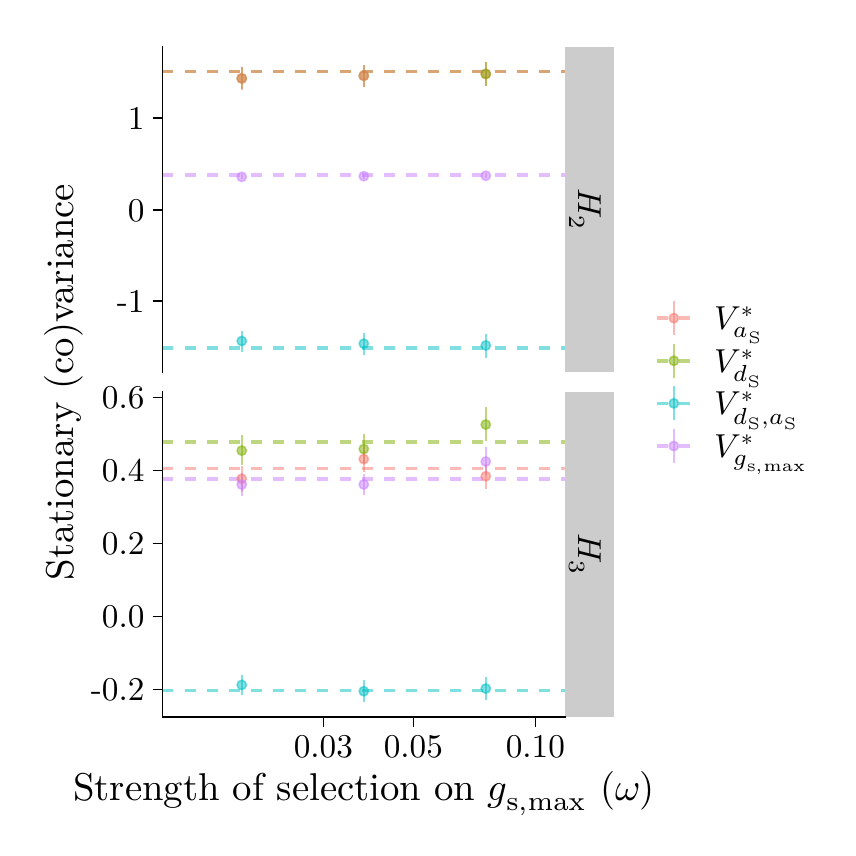
\begin{tikzpicture}[x=1pt,y=1pt]
\definecolor{fillColor}{RGB}{255,255,255}
\path[use as bounding box,fill=fillColor,fill opacity=0.00] (0,0) rectangle (289.08,289.08);
\begin{scope}
\path[clip] ( 48.69,164.52) rectangle (194.20,282.08);
\definecolor{drawColor}{RGB}{124,174,0}

\path[draw=drawColor,draw opacity=0.50,line width= 1.3pt,dash pattern=on 4pt off 4pt ,line join=round] ( 48.69,273.24) -- (194.20,273.24);
\definecolor{drawColor}{RGB}{248,118,109}

\path[draw=drawColor,draw opacity=0.50,line width= 1.3pt,dash pattern=on 4pt off 4pt ,line join=round] ( 48.69,273.24) -- (194.20,273.24);
\definecolor{drawColor}{RGB}{0,191,196}

\path[draw=drawColor,draw opacity=0.50,line width= 1.3pt,dash pattern=on 4pt off 4pt ,line join=round] ( 48.69,173.36) -- (194.20,173.36);
\definecolor{drawColor}{RGB}{199,124,255}

\path[draw=drawColor,draw opacity=0.50,line width= 1.3pt,dash pattern=on 4pt off 4pt ,line join=round] ( 48.69,235.79) -- (194.20,235.79);
\definecolor{drawColor}{RGB}{248,118,109}

\path[draw=drawColor,draw opacity=0.50,line width= 0.7pt,line join=round] (165.54,268.03) -- (165.54,276.74);
\definecolor{drawColor}{RGB}{124,174,0}

\path[draw=drawColor,draw opacity=0.50,line width= 0.7pt,line join=round] (165.54,268.02) -- (165.54,276.69);
\definecolor{drawColor}{RGB}{0,191,196}

\path[draw=drawColor,draw opacity=0.50,line width= 0.7pt,line join=round] (165.54,169.86) -- (165.54,178.41);
\definecolor{drawColor}{RGB}{124,174,0}

\path[draw=drawColor,draw opacity=0.50,line width= 0.7pt,line join=round] ( 77.35,266.93) -- ( 77.35,275.03);
\definecolor{drawColor}{RGB}{248,118,109}

\path[draw=drawColor,draw opacity=0.50,line width= 0.7pt,line join=round] ( 77.35,266.70) -- ( 77.35,274.78);
\definecolor{drawColor}{RGB}{124,174,0}

\path[draw=drawColor,draw opacity=0.50,line width= 0.7pt,line join=round] (121.45,267.76) -- (121.45,275.69);
\definecolor{drawColor}{RGB}{248,118,109}

\path[draw=drawColor,draw opacity=0.50,line width= 0.7pt,line join=round] (121.45,267.50) -- (121.45,275.42);
\definecolor{drawColor}{RGB}{0,191,196}

\path[draw=drawColor,draw opacity=0.50,line width= 0.7pt,line join=round] (121.45,170.78) -- (121.45,178.68);

\path[draw=drawColor,draw opacity=0.50,line width= 0.7pt,line join=round] ( 77.35,171.98) -- ( 77.35,179.55);
\definecolor{drawColor}{RGB}{199,124,255}

\path[draw=drawColor,draw opacity=0.50,line width= 0.7pt,line join=round] (165.54,234.59) -- (165.54,236.67);

\path[draw=drawColor,draw opacity=0.50,line width= 0.7pt,line join=round] (121.45,234.40) -- (121.45,236.38);

\path[draw=drawColor,draw opacity=0.50,line width= 0.7pt,line join=round] ( 77.35,234.27) -- ( 77.35,236.12);
\definecolor{drawColor}{RGB}{248,118,109}
\definecolor{fillColor}{RGB}{248,118,109}

\path[draw=drawColor,draw opacity=0.50,line width= 0.6pt,line join=round,line cap=round,fill=fillColor,fill opacity=0.50] (165.54,272.35) circle (  1.69);
\definecolor{drawColor}{RGB}{124,174,0}
\definecolor{fillColor}{RGB}{124,174,0}

\path[draw=drawColor,draw opacity=0.50,line width= 0.6pt,line join=round,line cap=round,fill=fillColor,fill opacity=0.50] (165.54,272.36) circle (  1.69);
\definecolor{drawColor}{RGB}{0,191,196}
\definecolor{fillColor}{RGB}{0,191,196}

\path[draw=drawColor,draw opacity=0.50,line width= 0.6pt,line join=round,line cap=round,fill=fillColor,fill opacity=0.50] (165.54,174.25) circle (  1.69);
\definecolor{drawColor}{RGB}{124,174,0}
\definecolor{fillColor}{RGB}{124,174,0}

\path[draw=drawColor,draw opacity=0.50,line width= 0.6pt,line join=round,line cap=round,fill=fillColor,fill opacity=0.50] ( 77.35,270.74) circle (  1.69);
\definecolor{drawColor}{RGB}{248,118,109}
\definecolor{fillColor}{RGB}{248,118,109}

\path[draw=drawColor,draw opacity=0.50,line width= 0.6pt,line join=round,line cap=round,fill=fillColor,fill opacity=0.50] ( 77.35,270.76) circle (  1.69);
\definecolor{drawColor}{RGB}{124,174,0}
\definecolor{fillColor}{RGB}{124,174,0}

\path[draw=drawColor,draw opacity=0.50,line width= 0.6pt,line join=round,line cap=round,fill=fillColor,fill opacity=0.50] (121.45,271.70) circle (  1.69);
\definecolor{drawColor}{RGB}{248,118,109}
\definecolor{fillColor}{RGB}{248,118,109}

\path[draw=drawColor,draw opacity=0.50,line width= 0.6pt,line join=round,line cap=round,fill=fillColor,fill opacity=0.50] (121.45,271.72) circle (  1.69);
\definecolor{drawColor}{RGB}{0,191,196}
\definecolor{fillColor}{RGB}{0,191,196}

\path[draw=drawColor,draw opacity=0.50,line width= 0.6pt,line join=round,line cap=round,fill=fillColor,fill opacity=0.50] (121.45,174.89) circle (  1.69);

\path[draw=drawColor,draw opacity=0.50,line width= 0.6pt,line join=round,line cap=round,fill=fillColor,fill opacity=0.50] ( 77.35,175.85) circle (  1.69);
\definecolor{drawColor}{RGB}{199,124,255}
\definecolor{fillColor}{RGB}{199,124,255}

\path[draw=drawColor,draw opacity=0.50,line width= 0.6pt,line join=round,line cap=round,fill=fillColor,fill opacity=0.50] (165.54,235.57) circle (  1.69);

\path[draw=drawColor,draw opacity=0.50,line width= 0.6pt,line join=round,line cap=round,fill=fillColor,fill opacity=0.50] (121.45,235.40) circle (  1.69);

\path[draw=drawColor,draw opacity=0.50,line width= 0.6pt,line join=round,line cap=round,fill=fillColor,fill opacity=0.50] ( 77.35,235.16) circle (  1.69);
\end{scope}
\begin{scope}
\path[clip] ( 48.69, 39.96) rectangle (194.20,157.52);
\definecolor{drawColor}{RGB}{124,174,0}

\path[draw=drawColor,draw opacity=0.50,line width= 1.3pt,dash pattern=on 4pt off 4pt ,line join=round] ( 48.69,139.44) -- (194.20,139.44);
\definecolor{drawColor}{RGB}{248,118,109}

\path[draw=drawColor,draw opacity=0.50,line width= 1.3pt,dash pattern=on 4pt off 4pt ,line join=round] ( 48.69,129.72) -- (194.20,129.72);
\definecolor{drawColor}{RGB}{0,191,196}

\path[draw=drawColor,draw opacity=0.50,line width= 1.3pt,dash pattern=on 4pt off 4pt ,line join=round] ( 48.69, 49.61) -- (194.20, 49.61);
\definecolor{drawColor}{RGB}{199,124,255}

\path[draw=drawColor,draw opacity=0.50,line width= 1.3pt,dash pattern=on 4pt off 4pt ,line join=round] ( 48.69,126.09) -- (194.20,126.09);
\definecolor{drawColor}{RGB}{124,174,0}

\path[draw=drawColor,draw opacity=0.50,line width= 0.7pt,line join=round] (165.54,139.61) -- (165.54,152.18);

\path[draw=drawColor,draw opacity=0.50,line width= 0.7pt,line join=round] ( 77.35,131.15) -- ( 77.35,141.79);

\path[draw=drawColor,draw opacity=0.50,line width= 0.7pt,line join=round] (121.45,131.95) -- (121.45,142.32);
\definecolor{drawColor}{RGB}{199,124,255}

\path[draw=drawColor,draw opacity=0.50,line width= 0.7pt,line join=round] (165.54,127.30) -- (165.54,137.52);
\definecolor{drawColor}{RGB}{248,118,109}

\path[draw=drawColor,draw opacity=0.50,line width= 0.7pt,line join=round] ( 77.35,121.32) -- ( 77.35,130.64);

\path[draw=drawColor,draw opacity=0.50,line width= 0.7pt,line join=round] (165.54,122.33) -- (165.54,131.49);

\path[draw=drawColor,draw opacity=0.50,line width= 0.7pt,line join=round] (121.45,128.67) -- (121.45,137.74);
\definecolor{drawColor}{RGB}{199,124,255}

\path[draw=drawColor,draw opacity=0.50,line width= 0.7pt,line join=round] ( 77.35,119.77) -- ( 77.35,128.03);
\definecolor{drawColor}{RGB}{0,191,196}

\path[draw=drawColor,draw opacity=0.50,line width= 0.7pt,line join=round] (165.54, 46.19) -- (165.54, 54.27);

\path[draw=drawColor,draw opacity=0.50,line width= 0.7pt,line join=round] (121.45, 45.30) -- (121.45, 53.36);
\definecolor{drawColor}{RGB}{199,124,255}

\path[draw=drawColor,draw opacity=0.50,line width= 0.7pt,line join=round] (121.45,120.12) -- (121.45,127.87);
\definecolor{drawColor}{RGB}{0,191,196}

\path[draw=drawColor,draw opacity=0.50,line width= 0.7pt,line join=round] ( 77.35, 47.97) -- ( 77.35, 55.30);
\definecolor{drawColor}{RGB}{124,174,0}
\definecolor{fillColor}{RGB}{124,174,0}

\path[draw=drawColor,draw opacity=0.50,line width= 0.6pt,line join=round,line cap=round,fill=fillColor,fill opacity=0.50] (165.54,145.66) circle (  1.69);

\path[draw=drawColor,draw opacity=0.50,line width= 0.6pt,line join=round,line cap=round,fill=fillColor,fill opacity=0.50] ( 77.35,136.26) circle (  1.69);

\path[draw=drawColor,draw opacity=0.50,line width= 0.6pt,line join=round,line cap=round,fill=fillColor,fill opacity=0.50] (121.45,136.82) circle (  1.69);
\definecolor{drawColor}{RGB}{199,124,255}
\definecolor{fillColor}{RGB}{199,124,255}

\path[draw=drawColor,draw opacity=0.50,line width= 0.6pt,line join=round,line cap=round,fill=fillColor,fill opacity=0.50] (165.54,132.29) circle (  1.69);
\definecolor{drawColor}{RGB}{248,118,109}
\definecolor{fillColor}{RGB}{248,118,109}

\path[draw=drawColor,draw opacity=0.50,line width= 0.6pt,line join=round,line cap=round,fill=fillColor,fill opacity=0.50] ( 77.35,126.08) circle (  1.69);

\path[draw=drawColor,draw opacity=0.50,line width= 0.6pt,line join=round,line cap=round,fill=fillColor,fill opacity=0.50] (165.54,126.99) circle (  1.69);

\path[draw=drawColor,draw opacity=0.50,line width= 0.6pt,line join=round,line cap=round,fill=fillColor,fill opacity=0.50] (121.45,133.19) circle (  1.69);
\definecolor{drawColor}{RGB}{199,124,255}
\definecolor{fillColor}{RGB}{199,124,255}

\path[draw=drawColor,draw opacity=0.50,line width= 0.6pt,line join=round,line cap=round,fill=fillColor,fill opacity=0.50] ( 77.35,123.98) circle (  1.69);
\definecolor{drawColor}{RGB}{0,191,196}
\definecolor{fillColor}{RGB}{0,191,196}

\path[draw=drawColor,draw opacity=0.50,line width= 0.6pt,line join=round,line cap=round,fill=fillColor,fill opacity=0.50] (165.54, 50.28) circle (  1.69);

\path[draw=drawColor,draw opacity=0.50,line width= 0.6pt,line join=round,line cap=round,fill=fillColor,fill opacity=0.50] (121.45, 49.30) circle (  1.69);
\definecolor{drawColor}{RGB}{199,124,255}
\definecolor{fillColor}{RGB}{199,124,255}

\path[draw=drawColor,draw opacity=0.50,line width= 0.6pt,line join=round,line cap=round,fill=fillColor,fill opacity=0.50] (121.45,124.02) circle (  1.69);
\definecolor{drawColor}{RGB}{0,191,196}
\definecolor{fillColor}{RGB}{0,191,196}

\path[draw=drawColor,draw opacity=0.50,line width= 0.6pt,line join=round,line cap=round,fill=fillColor,fill opacity=0.50] ( 77.35, 51.59) circle (  1.69);
\end{scope}
\begin{scope}
\path[clip] (194.20,164.52) rectangle (211.80,282.08);
\definecolor{fillColor}{gray}{0.80}

\path[fill=fillColor] (194.20,164.52) rectangle (211.80,282.08);
\definecolor{drawColor}{RGB}{0,0,0}

\node[text=drawColor,rotate=-90.00,anchor=base,inner sep=0pt, outer sep=0pt, scale=  1.20] at (198.87,223.30) {$H_2$};
\end{scope}
\begin{scope}
\path[clip] (194.20, 39.96) rectangle (211.80,157.52);
\definecolor{fillColor}{gray}{0.80}

\path[fill=fillColor] (194.20, 39.96) rectangle (211.80,157.52);
\definecolor{drawColor}{RGB}{0,0,0}

\node[text=drawColor,rotate=-90.00,anchor=base,inner sep=0pt, outer sep=0pt, scale=  1.20] at (198.87, 98.74) {$H_3$};
\end{scope}
\begin{scope}
\path[clip] (  0.00,  0.00) rectangle (289.08,289.08);
\definecolor{drawColor}{RGB}{0,0,0}

\path[draw=drawColor,line width= 0.6pt,line join=round,line cap=rect] ( 48.69, 39.96) --
	(194.20, 39.96);
\end{scope}
\begin{scope}
\path[clip] (  0.00,  0.00) rectangle (289.08,289.08);
\definecolor{drawColor}{RGB}{0,0,0}

\path[draw=drawColor,line width= 0.6pt,line join=round] (106.86, 36.46) --
	(106.86, 39.96);

\path[draw=drawColor,line width= 0.6pt,line join=round] (139.36, 36.46) --
	(139.36, 39.96);

\path[draw=drawColor,line width= 0.6pt,line join=round] (183.45, 36.46) --
	(183.45, 39.96);
\end{scope}
\begin{scope}
\path[clip] (  0.00,  0.00) rectangle (289.08,289.08);
\definecolor{drawColor}{RGB}{0,0,0}

\node[text=drawColor,anchor=base,inner sep=0pt, outer sep=0pt, scale=  1.20] at (106.86, 25.20) {0.03};

\node[text=drawColor,anchor=base,inner sep=0pt, outer sep=0pt, scale=  1.20] at (139.36, 25.20) {0.05};

\node[text=drawColor,anchor=base,inner sep=0pt, outer sep=0pt, scale=  1.20] at (183.45, 25.20) {0.10};
\end{scope}
\begin{scope}
\path[clip] (  0.00,  0.00) rectangle (289.08,289.08);
\definecolor{drawColor}{RGB}{0,0,0}

\path[draw=drawColor,line width= 0.6pt,line join=round,line cap=rect] ( 48.69,164.52) --
	( 48.69,282.08);
\end{scope}
\begin{scope}
\path[clip] (  0.00,  0.00) rectangle (289.08,289.08);
\definecolor{drawColor}{RGB}{0,0,0}

\node[text=drawColor,anchor=base east,inner sep=0pt, outer sep=0pt, scale=  1.20] at ( 42.19,186.08) {-1};

\node[text=drawColor,anchor=base east,inner sep=0pt, outer sep=0pt, scale=  1.20] at ( 42.19,219.17) {0};

\node[text=drawColor,anchor=base east,inner sep=0pt, outer sep=0pt, scale=  1.20] at ( 42.19,252.26) {1};
\end{scope}
\begin{scope}
\path[clip] (  0.00,  0.00) rectangle (289.08,289.08);
\definecolor{drawColor}{RGB}{0,0,0}

\path[draw=drawColor,line width= 0.6pt,line join=round] ( 45.19,190.21) --
	( 48.69,190.21);

\path[draw=drawColor,line width= 0.6pt,line join=round] ( 45.19,223.30) --
	( 48.69,223.30);

\path[draw=drawColor,line width= 0.6pt,line join=round] ( 45.19,256.39) --
	( 48.69,256.39);
\end{scope}
\begin{scope}
\path[clip] (  0.00,  0.00) rectangle (289.08,289.08);
\definecolor{drawColor}{RGB}{0,0,0}

\path[draw=drawColor,line width= 0.6pt,line join=round,line cap=rect] ( 48.69, 39.96) --
	( 48.69,157.52);
\end{scope}
\begin{scope}
\path[clip] (  0.00,  0.00) rectangle (289.08,289.08);
\definecolor{drawColor}{RGB}{0,0,0}

\node[text=drawColor,anchor=base east,inner sep=0pt, outer sep=0pt, scale=  1.20] at ( 42.19, 45.79) {-0.2};

\node[text=drawColor,anchor=base east,inner sep=0pt, outer sep=0pt, scale=  1.20] at ( 42.19, 72.18) {0.0};

\node[text=drawColor,anchor=base east,inner sep=0pt, outer sep=0pt, scale=  1.20] at ( 42.19, 98.57) {0.2};

\node[text=drawColor,anchor=base east,inner sep=0pt, outer sep=0pt, scale=  1.20] at ( 42.19,124.95) {0.4};

\node[text=drawColor,anchor=base east,inner sep=0pt, outer sep=0pt, scale=  1.20] at ( 42.19,151.34) {0.6};
\end{scope}
\begin{scope}
\path[clip] (  0.00,  0.00) rectangle (289.08,289.08);
\definecolor{drawColor}{RGB}{0,0,0}

\path[draw=drawColor,line width= 0.6pt,line join=round] ( 45.19, 49.93) --
	( 48.69, 49.93);

\path[draw=drawColor,line width= 0.6pt,line join=round] ( 45.19, 76.31) --
	( 48.69, 76.31);

\path[draw=drawColor,line width= 0.6pt,line join=round] ( 45.19,102.70) --
	( 48.69,102.70);

\path[draw=drawColor,line width= 0.6pt,line join=round] ( 45.19,129.08) --
	( 48.69,129.08);

\path[draw=drawColor,line width= 0.6pt,line join=round] ( 45.19,155.47) --
	( 48.69,155.47);
\end{scope}
\begin{scope}
\path[clip] (  0.00,  0.00) rectangle (289.08,289.08);
\definecolor{drawColor}{RGB}{0,0,0}

\node[text=drawColor,anchor=base,inner sep=0pt, outer sep=0pt, scale=  1.40] at (121.45,  9.72) {Strength of selection on $g_\mathrm{s,max}$ ($\omega$)};
\end{scope}
\begin{scope}
\path[clip] (  0.00,  0.00) rectangle (289.08,289.08);
\definecolor{drawColor}{RGB}{0,0,0}

\node[text=drawColor,rotate= 90.00,anchor=base,inner sep=0pt, outer sep=0pt, scale=  1.40] at ( 16.64,161.02) {Stationary (co)variance};
\end{scope}
\begin{scope}
\path[clip] (  0.00,  0.00) rectangle (289.08,289.08);
\definecolor{drawColor}{RGB}{248,118,109}

\path[draw=drawColor,draw opacity=0.50,line width= 1.3pt,dash pattern=on 4pt off 4pt ,line join=round] (227.34,184.12) -- (239.66,184.12);
\end{scope}
\begin{scope}
\path[clip] (  0.00,  0.00) rectangle (289.08,289.08);
\definecolor{drawColor}{RGB}{248,118,109}

\path[draw=drawColor,draw opacity=0.50,line width= 0.7pt,line join=round] (233.50,177.96) -- (233.50,190.28);
\definecolor{fillColor}{RGB}{248,118,109}

\path[draw=drawColor,draw opacity=0.50,line width= 0.6pt,line join=round,line cap=round,fill=fillColor,fill opacity=0.50] (233.50,184.12) circle (  1.69);
\end{scope}
\begin{scope}
\path[clip] (  0.00,  0.00) rectangle (289.08,289.08);
\definecolor{drawColor}{RGB}{124,174,0}

\path[draw=drawColor,draw opacity=0.50,line width= 1.3pt,dash pattern=on 4pt off 4pt ,line join=round] (227.34,168.72) -- (239.66,168.72);
\end{scope}
\begin{scope}
\path[clip] (  0.00,  0.00) rectangle (289.08,289.08);
\definecolor{drawColor}{RGB}{124,174,0}

\path[draw=drawColor,draw opacity=0.50,line width= 0.7pt,line join=round] (233.50,162.56) -- (233.50,174.88);
\definecolor{fillColor}{RGB}{124,174,0}

\path[draw=drawColor,draw opacity=0.50,line width= 0.6pt,line join=round,line cap=round,fill=fillColor,fill opacity=0.50] (233.50,168.72) circle (  1.69);
\end{scope}
\begin{scope}
\path[clip] (  0.00,  0.00) rectangle (289.08,289.08);
\definecolor{drawColor}{RGB}{0,191,196}

\path[draw=drawColor,draw opacity=0.50,line width= 1.3pt,dash pattern=on 4pt off 4pt ,line join=round] (227.34,153.32) -- (239.66,153.32);
\end{scope}
\begin{scope}
\path[clip] (  0.00,  0.00) rectangle (289.08,289.08);
\definecolor{drawColor}{RGB}{0,191,196}

\path[draw=drawColor,draw opacity=0.50,line width= 0.7pt,line join=round] (233.50,147.16) -- (233.50,159.48);
\definecolor{fillColor}{RGB}{0,191,196}

\path[draw=drawColor,draw opacity=0.50,line width= 0.6pt,line join=round,line cap=round,fill=fillColor,fill opacity=0.50] (233.50,153.32) circle (  1.69);
\end{scope}
\begin{scope}
\path[clip] (  0.00,  0.00) rectangle (289.08,289.08);
\definecolor{drawColor}{RGB}{199,124,255}

\path[draw=drawColor,draw opacity=0.50,line width= 1.3pt,dash pattern=on 4pt off 4pt ,line join=round] (227.34,137.92) -- (239.66,137.92);
\end{scope}
\begin{scope}
\path[clip] (  0.00,  0.00) rectangle (289.08,289.08);
\definecolor{drawColor}{RGB}{199,124,255}

\path[draw=drawColor,draw opacity=0.50,line width= 0.7pt,line join=round] (233.50,131.76) -- (233.50,144.08);
\definecolor{fillColor}{RGB}{199,124,255}

\path[draw=drawColor,draw opacity=0.50,line width= 0.6pt,line join=round,line cap=round,fill=fillColor,fill opacity=0.50] (233.50,137.92) circle (  1.69);
\end{scope}
\begin{scope}
\path[clip] (  0.00,  0.00) rectangle (289.08,289.08);
\definecolor{drawColor}{RGB}{0,0,0}

\node[text=drawColor,anchor=base west,inner sep=0pt, outer sep=0pt, scale=  1.20] at (248.20,179.99) {$V^*_{a_\mathrm{S}}$};
\end{scope}
\begin{scope}
\path[clip] (  0.00,  0.00) rectangle (289.08,289.08);
\definecolor{drawColor}{RGB}{0,0,0}

\node[text=drawColor,anchor=base west,inner sep=0pt, outer sep=0pt, scale=  1.20] at (248.20,164.59) {$V^*_{d_\mathrm{S}}$};
\end{scope}
\begin{scope}
\path[clip] (  0.00,  0.00) rectangle (289.08,289.08);
\definecolor{drawColor}{RGB}{0,0,0}

\node[text=drawColor,anchor=base west,inner sep=0pt, outer sep=0pt, scale=  1.20] at (248.20,149.19) {$V^*_{d_\mathrm{S},a_\mathrm{S}}$};
\end{scope}
\begin{scope}
\path[clip] (  0.00,  0.00) rectangle (289.08,289.08);
\definecolor{drawColor}{RGB}{0,0,0}

\node[text=drawColor,anchor=base west,inner sep=0pt, outer sep=0pt, scale=  1.20] at (248.20,133.79) {$V^*_{g_\mathrm{s,max}}$};
\end{scope}
\end{tikzpicture}

\end{figure}

\newpage

\begin{figure}
\caption{Among-species trait (co)variances are not sensitive to the strength of selection on $\phi_f$ at stationarity. Dashed lines are the theoretical expectations for the interspecific variance in stomatal density ($V_{d_\mathrm{S}}^*$), stomatal size ($V_{a_\mathrm{S}}^*$), anatomical maximum stomatal conductance ($V_{g_\mathrm{s,max}}^*$), and covariance between density and size ($V_{d_\mathrm{S},a_\mathrm{S}}^*$) at stationarity. The theoretical expectations differ between the hypotheses, $H_2$: stomatal-area minimization (upper panel) and $H_3$: stomatal adaptation + bounded size (lower panel). The points are estimated from simulations of an ensemble of 1000 over a range of selection strengths ($\phi_f$), where a value of 1 corresponds to the baseline scenario. The solid line behind each points indicates the 95\% bootstrap confidence interval. All other parameters are set to their baseline value as described in the ``Baseline parameter values'' subsection.}
% Created by tikzDevice version 0.12.6 on 2025-08-19 18:36:12
% !TEX encoding = UTF-8 Unicode
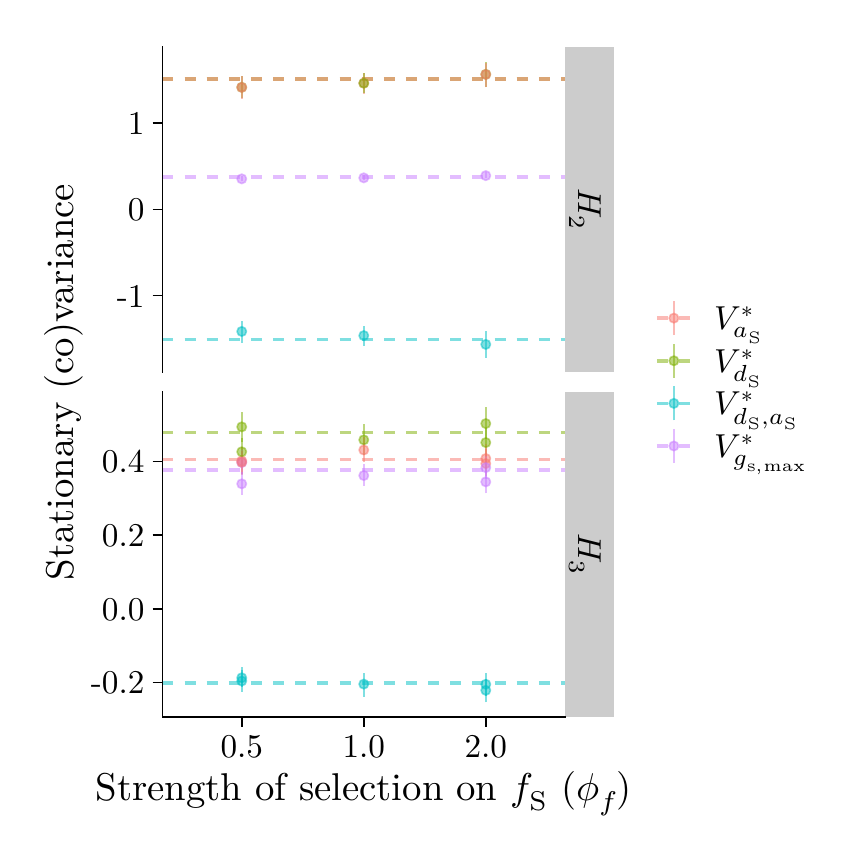
\begin{tikzpicture}[x=1pt,y=1pt]
\definecolor{fillColor}{RGB}{255,255,255}
\path[use as bounding box,fill=fillColor,fill opacity=0.00] (0,0) rectangle (289.08,289.08);
\begin{scope}
\path[clip] ( 48.69,164.52) rectangle (194.20,282.08);
\definecolor{drawColor}{RGB}{124,174,0}

\path[draw=drawColor,draw opacity=0.50,line width= 1.3pt,dash pattern=on 4pt off 4pt ,line join=round] ( 48.69,270.45) -- (194.20,270.45);
\definecolor{drawColor}{RGB}{248,118,109}

\path[draw=drawColor,draw opacity=0.50,line width= 1.3pt,dash pattern=on 4pt off 4pt ,line join=round] ( 48.69,270.45) -- (194.20,270.45);
\definecolor{drawColor}{RGB}{0,191,196}

\path[draw=drawColor,draw opacity=0.50,line width= 1.3pt,dash pattern=on 4pt off 4pt ,line join=round] ( 48.69,176.37) -- (194.20,176.37);
\definecolor{drawColor}{RGB}{199,124,255}

\path[draw=drawColor,draw opacity=0.50,line width= 1.3pt,dash pattern=on 4pt off 4pt ,line join=round] ( 48.69,235.17) -- (194.20,235.17);
\definecolor{drawColor}{RGB}{0,191,196}

\path[draw=drawColor,draw opacity=0.50,line width= 0.7pt,line join=round] (165.54,169.86) -- (165.54,179.30);
\definecolor{drawColor}{RGB}{124,174,0}

\path[draw=drawColor,draw opacity=0.50,line width= 0.7pt,line join=round] (165.54,267.59) -- (165.54,276.74);
\definecolor{drawColor}{RGB}{248,118,109}

\path[draw=drawColor,draw opacity=0.50,line width= 0.7pt,line join=round] (165.54,267.47) -- (165.54,276.48);
\definecolor{drawColor}{RGB}{124,174,0}

\path[draw=drawColor,draw opacity=0.50,line width= 0.7pt,line join=round] ( 77.35,263.50) -- ( 77.35,271.70);
\definecolor{drawColor}{RGB}{248,118,109}

\path[draw=drawColor,draw opacity=0.50,line width= 0.7pt,line join=round] ( 77.35,263.43) -- ( 77.35,271.46);
\definecolor{drawColor}{RGB}{0,191,196}

\path[draw=drawColor,draw opacity=0.50,line width= 0.7pt,line join=round] ( 77.35,175.23) -- ( 77.35,182.92);
\definecolor{drawColor}{RGB}{248,118,109}

\path[draw=drawColor,draw opacity=0.50,line width= 0.7pt,line join=round] (121.45,265.15) -- (121.45,272.68);
\definecolor{drawColor}{RGB}{0,191,196}

\path[draw=drawColor,draw opacity=0.50,line width= 0.7pt,line join=round] (121.45,174.00) -- (121.45,181.40);
\definecolor{drawColor}{RGB}{124,174,0}

\path[draw=drawColor,draw opacity=0.50,line width= 0.7pt,line join=round] (121.45,265.38) -- (121.45,272.59);
\definecolor{drawColor}{RGB}{199,124,255}

\path[draw=drawColor,draw opacity=0.50,line width= 0.7pt,line join=round] (165.54,234.62) -- (165.54,236.79);

\path[draw=drawColor,draw opacity=0.50,line width= 0.7pt,line join=round] ( 77.35,233.53) -- ( 77.35,235.45);

\path[draw=drawColor,draw opacity=0.50,line width= 0.7pt,line join=round] (121.45,233.91) -- (121.45,235.78);
\definecolor{drawColor}{RGB}{0,191,196}
\definecolor{fillColor}{RGB}{0,191,196}

\path[draw=drawColor,draw opacity=0.50,line width= 0.6pt,line join=round,line cap=round,fill=fillColor,fill opacity=0.50] (165.54,174.63) circle (  1.69);
\definecolor{drawColor}{RGB}{124,174,0}
\definecolor{fillColor}{RGB}{124,174,0}

\path[draw=drawColor,draw opacity=0.50,line width= 0.6pt,line join=round,line cap=round,fill=fillColor,fill opacity=0.50] (165.54,272.21) circle (  1.69);
\definecolor{drawColor}{RGB}{248,118,109}
\definecolor{fillColor}{RGB}{248,118,109}

\path[draw=drawColor,draw opacity=0.50,line width= 0.6pt,line join=round,line cap=round,fill=fillColor,fill opacity=0.50] (165.54,272.18) circle (  1.69);
\definecolor{drawColor}{RGB}{124,174,0}
\definecolor{fillColor}{RGB}{124,174,0}

\path[draw=drawColor,draw opacity=0.50,line width= 0.6pt,line join=round,line cap=round,fill=fillColor,fill opacity=0.50] ( 77.35,267.53) circle (  1.69);
\definecolor{drawColor}{RGB}{248,118,109}
\definecolor{fillColor}{RGB}{248,118,109}

\path[draw=drawColor,draw opacity=0.50,line width= 0.6pt,line join=round,line cap=round,fill=fillColor,fill opacity=0.50] ( 77.35,267.51) circle (  1.69);
\definecolor{drawColor}{RGB}{0,191,196}
\definecolor{fillColor}{RGB}{0,191,196}

\path[draw=drawColor,draw opacity=0.50,line width= 0.6pt,line join=round,line cap=round,fill=fillColor,fill opacity=0.50] ( 77.35,179.31) circle (  1.69);
\definecolor{drawColor}{RGB}{248,118,109}
\definecolor{fillColor}{RGB}{248,118,109}

\path[draw=drawColor,draw opacity=0.50,line width= 0.6pt,line join=round,line cap=round,fill=fillColor,fill opacity=0.50] (121.45,269.02) circle (  1.69);
\definecolor{drawColor}{RGB}{0,191,196}
\definecolor{fillColor}{RGB}{0,191,196}

\path[draw=drawColor,draw opacity=0.50,line width= 0.6pt,line join=round,line cap=round,fill=fillColor,fill opacity=0.50] (121.45,177.81) circle (  1.69);
\definecolor{drawColor}{RGB}{124,174,0}
\definecolor{fillColor}{RGB}{124,174,0}

\path[draw=drawColor,draw opacity=0.50,line width= 0.6pt,line join=round,line cap=round,fill=fillColor,fill opacity=0.50] (121.45,269.01) circle (  1.69);
\definecolor{drawColor}{RGB}{199,124,255}
\definecolor{fillColor}{RGB}{199,124,255}

\path[draw=drawColor,draw opacity=0.50,line width= 0.6pt,line join=round,line cap=round,fill=fillColor,fill opacity=0.50] (165.54,235.62) circle (  1.69);

\path[draw=drawColor,draw opacity=0.50,line width= 0.6pt,line join=round,line cap=round,fill=fillColor,fill opacity=0.50] ( 77.35,234.45) circle (  1.69);

\path[draw=drawColor,draw opacity=0.50,line width= 0.6pt,line join=round,line cap=round,fill=fillColor,fill opacity=0.50] (121.45,234.81) circle (  1.69);
\end{scope}
\begin{scope}
\path[clip] ( 48.69, 39.96) rectangle (194.20,157.52);
\definecolor{drawColor}{RGB}{124,174,0}

\path[draw=drawColor,draw opacity=0.50,line width= 1.3pt,dash pattern=on 4pt off 4pt ,line join=round] ( 48.69,142.78) -- (194.20,142.78);
\definecolor{drawColor}{RGB}{248,118,109}

\path[draw=drawColor,draw opacity=0.50,line width= 1.3pt,dash pattern=on 4pt off 4pt ,line join=round] ( 48.69,132.98) -- (194.20,132.98);
\definecolor{drawColor}{RGB}{0,191,196}

\path[draw=drawColor,draw opacity=0.50,line width= 1.3pt,dash pattern=on 4pt off 4pt ,line join=round] ( 48.69, 52.19) -- (194.20, 52.19);
\definecolor{drawColor}{RGB}{199,124,255}

\path[draw=drawColor,draw opacity=0.50,line width= 1.3pt,dash pattern=on 4pt off 4pt ,line join=round] ( 48.69,129.32) -- (194.20,129.32);
\definecolor{drawColor}{RGB}{124,174,0}

\path[draw=drawColor,draw opacity=0.50,line width= 0.7pt,line join=round] (165.54,140.53) -- (165.54,152.18);

\path[draw=drawColor,draw opacity=0.50,line width= 0.7pt,line join=round] (121.45,134.79) -- (121.45,145.72);

\path[draw=drawColor,draw opacity=0.50,line width= 0.7pt,line join=round] ( 77.35,139.22) -- ( 77.35,150.03);

\path[draw=drawColor,draw opacity=0.50,line width= 0.7pt,line join=round] (165.54,134.06) -- (165.54,144.28);
\definecolor{drawColor}{RGB}{248,118,109}

\path[draw=drawColor,draw opacity=0.50,line width= 0.7pt,line join=round] (165.54,128.56) -- (165.54,138.69);

\path[draw=drawColor,draw opacity=0.50,line width= 0.7pt,line join=round] ( 77.35,127.70) -- ( 77.35,137.71);
\definecolor{drawColor}{RGB}{124,174,0}

\path[draw=drawColor,draw opacity=0.50,line width= 0.7pt,line join=round] ( 77.35,130.86) -- ( 77.35,140.82);
\definecolor{drawColor}{RGB}{248,118,109}

\path[draw=drawColor,draw opacity=0.50,line width= 0.7pt,line join=round] (165.54,127.04) -- (165.54,136.74);

\path[draw=drawColor,draw opacity=0.50,line width= 0.7pt,line join=round] (121.45,132.07) -- (121.45,141.07);
\definecolor{drawColor}{RGB}{199,124,255}

\path[draw=drawColor,draw opacity=0.50,line width= 0.7pt,line join=round] ( 77.35,127.79) -- ( 77.35,136.57);
\definecolor{drawColor}{RGB}{248,118,109}

\path[draw=drawColor,draw opacity=0.50,line width= 0.7pt,line join=round] ( 77.35,127.54) -- ( 77.35,136.20);
\definecolor{drawColor}{RGB}{0,191,196}

\path[draw=drawColor,draw opacity=0.50,line width= 0.7pt,line join=round] (121.45, 47.23) -- (121.45, 55.86);

\path[draw=drawColor,draw opacity=0.50,line width= 0.7pt,line join=round] (165.54, 45.30) -- (165.54, 53.79);
\definecolor{drawColor}{RGB}{199,124,255}

\path[draw=drawColor,draw opacity=0.50,line width= 0.7pt,line join=round] (165.54,126.07) -- (165.54,134.38);

\path[draw=drawColor,draw opacity=0.50,line width= 0.7pt,line join=round] (121.45,123.38) -- (121.45,131.58);

\path[draw=drawColor,draw opacity=0.50,line width= 0.7pt,line join=round] ( 77.35,120.23) -- ( 77.35,128.37);

\path[draw=drawColor,draw opacity=0.50,line width= 0.7pt,line join=round] (165.54,120.78) -- (165.54,128.84);
\definecolor{drawColor}{RGB}{0,191,196}

\path[draw=drawColor,draw opacity=0.50,line width= 0.7pt,line join=round] (165.54, 47.73) -- (165.54, 55.72);

\path[draw=drawColor,draw opacity=0.50,line width= 0.7pt,line join=round] ( 77.35, 49.12) -- ( 77.35, 57.09);

\path[draw=drawColor,draw opacity=0.50,line width= 0.7pt,line join=round] ( 77.35, 50.84) -- ( 77.35, 57.90);
\definecolor{drawColor}{RGB}{124,174,0}
\definecolor{fillColor}{RGB}{124,174,0}

\path[draw=drawColor,draw opacity=0.50,line width= 0.6pt,line join=round,line cap=round,fill=fillColor,fill opacity=0.50] (165.54,146.02) circle (  1.69);

\path[draw=drawColor,draw opacity=0.50,line width= 0.6pt,line join=round,line cap=round,fill=fillColor,fill opacity=0.50] (121.45,140.14) circle (  1.69);

\path[draw=drawColor,draw opacity=0.50,line width= 0.6pt,line join=round,line cap=round,fill=fillColor,fill opacity=0.50] ( 77.35,144.83) circle (  1.69);

\path[draw=drawColor,draw opacity=0.50,line width= 0.6pt,line join=round,line cap=round,fill=fillColor,fill opacity=0.50] (165.54,139.16) circle (  1.69);
\definecolor{drawColor}{RGB}{248,118,109}
\definecolor{fillColor}{RGB}{248,118,109}

\path[draw=drawColor,draw opacity=0.50,line width= 0.6pt,line join=round,line cap=round,fill=fillColor,fill opacity=0.50] (165.54,133.40) circle (  1.69);

\path[draw=drawColor,draw opacity=0.50,line width= 0.6pt,line join=round,line cap=round,fill=fillColor,fill opacity=0.50] ( 77.35,132.59) circle (  1.69);
\definecolor{drawColor}{RGB}{124,174,0}
\definecolor{fillColor}{RGB}{124,174,0}

\path[draw=drawColor,draw opacity=0.50,line width= 0.6pt,line join=round,line cap=round,fill=fillColor,fill opacity=0.50] ( 77.35,135.84) circle (  1.69);
\definecolor{drawColor}{RGB}{248,118,109}
\definecolor{fillColor}{RGB}{248,118,109}

\path[draw=drawColor,draw opacity=0.50,line width= 0.6pt,line join=round,line cap=round,fill=fillColor,fill opacity=0.50] (165.54,131.58) circle (  1.69);

\path[draw=drawColor,draw opacity=0.50,line width= 0.6pt,line join=round,line cap=round,fill=fillColor,fill opacity=0.50] (121.45,136.48) circle (  1.69);
\definecolor{drawColor}{RGB}{199,124,255}
\definecolor{fillColor}{RGB}{199,124,255}

\path[draw=drawColor,draw opacity=0.50,line width= 0.6pt,line join=round,line cap=round,fill=fillColor,fill opacity=0.50] ( 77.35,131.93) circle (  1.69);
\definecolor{drawColor}{RGB}{248,118,109}
\definecolor{fillColor}{RGB}{248,118,109}

\path[draw=drawColor,draw opacity=0.50,line width= 0.6pt,line join=round,line cap=round,fill=fillColor,fill opacity=0.50] ( 77.35,132.05) circle (  1.69);
\definecolor{drawColor}{RGB}{0,191,196}
\definecolor{fillColor}{RGB}{0,191,196}

\path[draw=drawColor,draw opacity=0.50,line width= 0.6pt,line join=round,line cap=round,fill=fillColor,fill opacity=0.50] (121.45, 51.88) circle (  1.69);

\path[draw=drawColor,draw opacity=0.50,line width= 0.6pt,line join=round,line cap=round,fill=fillColor,fill opacity=0.50] (165.54, 49.63) circle (  1.69);
\definecolor{drawColor}{RGB}{199,124,255}
\definecolor{fillColor}{RGB}{199,124,255}

\path[draw=drawColor,draw opacity=0.50,line width= 0.6pt,line join=round,line cap=round,fill=fillColor,fill opacity=0.50] (165.54,130.11) circle (  1.69);

\path[draw=drawColor,draw opacity=0.50,line width= 0.6pt,line join=round,line cap=round,fill=fillColor,fill opacity=0.50] (121.45,127.24) circle (  1.69);

\path[draw=drawColor,draw opacity=0.50,line width= 0.6pt,line join=round,line cap=round,fill=fillColor,fill opacity=0.50] ( 77.35,124.25) circle (  1.69);

\path[draw=drawColor,draw opacity=0.50,line width= 0.6pt,line join=round,line cap=round,fill=fillColor,fill opacity=0.50] (165.54,124.96) circle (  1.69);
\definecolor{drawColor}{RGB}{0,191,196}
\definecolor{fillColor}{RGB}{0,191,196}

\path[draw=drawColor,draw opacity=0.50,line width= 0.6pt,line join=round,line cap=round,fill=fillColor,fill opacity=0.50] (165.54, 51.81) circle (  1.69);

\path[draw=drawColor,draw opacity=0.50,line width= 0.6pt,line join=round,line cap=round,fill=fillColor,fill opacity=0.50] ( 77.35, 53.00) circle (  1.69);

\path[draw=drawColor,draw opacity=0.50,line width= 0.6pt,line join=round,line cap=round,fill=fillColor,fill opacity=0.50] ( 77.35, 54.16) circle (  1.69);
\end{scope}
\begin{scope}
\path[clip] (194.20,164.52) rectangle (211.80,282.08);
\definecolor{fillColor}{gray}{0.80}

\path[fill=fillColor] (194.20,164.52) rectangle (211.80,282.08);
\definecolor{drawColor}{RGB}{0,0,0}

\node[text=drawColor,rotate=-90.00,anchor=base,inner sep=0pt, outer sep=0pt, scale=  1.20] at (198.87,223.30) {$H_2$};
\end{scope}
\begin{scope}
\path[clip] (194.20, 39.96) rectangle (211.80,157.52);
\definecolor{fillColor}{gray}{0.80}

\path[fill=fillColor] (194.20, 39.96) rectangle (211.80,157.52);
\definecolor{drawColor}{RGB}{0,0,0}

\node[text=drawColor,rotate=-90.00,anchor=base,inner sep=0pt, outer sep=0pt, scale=  1.20] at (198.87, 98.74) {$H_3$};
\end{scope}
\begin{scope}
\path[clip] (  0.00,  0.00) rectangle (289.08,289.08);
\definecolor{drawColor}{RGB}{0,0,0}

\path[draw=drawColor,line width= 0.6pt,line join=round,line cap=rect] ( 48.69, 39.96) --
	(194.20, 39.96);
\end{scope}
\begin{scope}
\path[clip] (  0.00,  0.00) rectangle (289.08,289.08);
\definecolor{drawColor}{RGB}{0,0,0}

\path[draw=drawColor,line width= 0.6pt,line join=round] ( 77.35, 36.46) --
	( 77.35, 39.96);

\path[draw=drawColor,line width= 0.6pt,line join=round] (121.45, 36.46) --
	(121.45, 39.96);

\path[draw=drawColor,line width= 0.6pt,line join=round] (165.54, 36.46) --
	(165.54, 39.96);
\end{scope}
\begin{scope}
\path[clip] (  0.00,  0.00) rectangle (289.08,289.08);
\definecolor{drawColor}{RGB}{0,0,0}

\node[text=drawColor,anchor=base,inner sep=0pt, outer sep=0pt, scale=  1.20] at ( 77.35, 25.20) {0.5};

\node[text=drawColor,anchor=base,inner sep=0pt, outer sep=0pt, scale=  1.20] at (121.45, 25.20) {1.0};

\node[text=drawColor,anchor=base,inner sep=0pt, outer sep=0pt, scale=  1.20] at (165.54, 25.20) {2.0};
\end{scope}
\begin{scope}
\path[clip] (  0.00,  0.00) rectangle (289.08,289.08);
\definecolor{drawColor}{RGB}{0,0,0}

\path[draw=drawColor,line width= 0.6pt,line join=round,line cap=rect] ( 48.69,164.52) --
	( 48.69,282.08);
\end{scope}
\begin{scope}
\path[clip] (  0.00,  0.00) rectangle (289.08,289.08);
\definecolor{drawColor}{RGB}{0,0,0}

\node[text=drawColor,anchor=base east,inner sep=0pt, outer sep=0pt, scale=  1.20] at ( 42.19,188.11) {-1};

\node[text=drawColor,anchor=base east,inner sep=0pt, outer sep=0pt, scale=  1.20] at ( 42.19,219.28) {0};

\node[text=drawColor,anchor=base east,inner sep=0pt, outer sep=0pt, scale=  1.20] at ( 42.19,250.45) {1};
\end{scope}
\begin{scope}
\path[clip] (  0.00,  0.00) rectangle (289.08,289.08);
\definecolor{drawColor}{RGB}{0,0,0}

\path[draw=drawColor,line width= 0.6pt,line join=round] ( 45.19,192.24) --
	( 48.69,192.24);

\path[draw=drawColor,line width= 0.6pt,line join=round] ( 45.19,223.41) --
	( 48.69,223.41);

\path[draw=drawColor,line width= 0.6pt,line join=round] ( 45.19,254.58) --
	( 48.69,254.58);
\end{scope}
\begin{scope}
\path[clip] (  0.00,  0.00) rectangle (289.08,289.08);
\definecolor{drawColor}{RGB}{0,0,0}

\path[draw=drawColor,line width= 0.6pt,line join=round,line cap=rect] ( 48.69, 39.96) --
	( 48.69,157.52);
\end{scope}
\begin{scope}
\path[clip] (  0.00,  0.00) rectangle (289.08,289.08);
\definecolor{drawColor}{RGB}{0,0,0}

\node[text=drawColor,anchor=base east,inner sep=0pt, outer sep=0pt, scale=  1.20] at ( 42.19, 48.38) {-0.2};

\node[text=drawColor,anchor=base east,inner sep=0pt, outer sep=0pt, scale=  1.20] at ( 42.19, 74.99) {0.0};

\node[text=drawColor,anchor=base east,inner sep=0pt, outer sep=0pt, scale=  1.20] at ( 42.19,101.60) {0.2};

\node[text=drawColor,anchor=base east,inner sep=0pt, outer sep=0pt, scale=  1.20] at ( 42.19,128.21) {0.4};
\end{scope}
\begin{scope}
\path[clip] (  0.00,  0.00) rectangle (289.08,289.08);
\definecolor{drawColor}{RGB}{0,0,0}

\path[draw=drawColor,line width= 0.6pt,line join=round] ( 45.19, 52.51) --
	( 48.69, 52.51);

\path[draw=drawColor,line width= 0.6pt,line join=round] ( 45.19, 79.12) --
	( 48.69, 79.12);

\path[draw=drawColor,line width= 0.6pt,line join=round] ( 45.19,105.73) --
	( 48.69,105.73);

\path[draw=drawColor,line width= 0.6pt,line join=round] ( 45.19,132.34) --
	( 48.69,132.34);
\end{scope}
\begin{scope}
\path[clip] (  0.00,  0.00) rectangle (289.08,289.08);
\definecolor{drawColor}{RGB}{0,0,0}

\node[text=drawColor,anchor=base,inner sep=0pt, outer sep=0pt, scale=  1.40] at (121.45,  9.72) {Strength of selection on $f_\mathrm{S}$ ($\phi_f$)};
\end{scope}
\begin{scope}
\path[clip] (  0.00,  0.00) rectangle (289.08,289.08);
\definecolor{drawColor}{RGB}{0,0,0}

\node[text=drawColor,rotate= 90.00,anchor=base,inner sep=0pt, outer sep=0pt, scale=  1.40] at ( 16.64,161.02) {Stationary (co)variance};
\end{scope}
\begin{scope}
\path[clip] (  0.00,  0.00) rectangle (289.08,289.08);
\definecolor{drawColor}{RGB}{248,118,109}

\path[draw=drawColor,draw opacity=0.50,line width= 1.3pt,dash pattern=on 4pt off 4pt ,line join=round] (227.34,184.12) -- (239.66,184.12);
\end{scope}
\begin{scope}
\path[clip] (  0.00,  0.00) rectangle (289.08,289.08);
\definecolor{drawColor}{RGB}{248,118,109}

\path[draw=drawColor,draw opacity=0.50,line width= 0.7pt,line join=round] (233.50,177.96) -- (233.50,190.28);
\definecolor{fillColor}{RGB}{248,118,109}

\path[draw=drawColor,draw opacity=0.50,line width= 0.6pt,line join=round,line cap=round,fill=fillColor,fill opacity=0.50] (233.50,184.12) circle (  1.69);
\end{scope}
\begin{scope}
\path[clip] (  0.00,  0.00) rectangle (289.08,289.08);
\definecolor{drawColor}{RGB}{124,174,0}

\path[draw=drawColor,draw opacity=0.50,line width= 1.3pt,dash pattern=on 4pt off 4pt ,line join=round] (227.34,168.72) -- (239.66,168.72);
\end{scope}
\begin{scope}
\path[clip] (  0.00,  0.00) rectangle (289.08,289.08);
\definecolor{drawColor}{RGB}{124,174,0}

\path[draw=drawColor,draw opacity=0.50,line width= 0.7pt,line join=round] (233.50,162.56) -- (233.50,174.88);
\definecolor{fillColor}{RGB}{124,174,0}

\path[draw=drawColor,draw opacity=0.50,line width= 0.6pt,line join=round,line cap=round,fill=fillColor,fill opacity=0.50] (233.50,168.72) circle (  1.69);
\end{scope}
\begin{scope}
\path[clip] (  0.00,  0.00) rectangle (289.08,289.08);
\definecolor{drawColor}{RGB}{0,191,196}

\path[draw=drawColor,draw opacity=0.50,line width= 1.3pt,dash pattern=on 4pt off 4pt ,line join=round] (227.34,153.32) -- (239.66,153.32);
\end{scope}
\begin{scope}
\path[clip] (  0.00,  0.00) rectangle (289.08,289.08);
\definecolor{drawColor}{RGB}{0,191,196}

\path[draw=drawColor,draw opacity=0.50,line width= 0.7pt,line join=round] (233.50,147.16) -- (233.50,159.48);
\definecolor{fillColor}{RGB}{0,191,196}

\path[draw=drawColor,draw opacity=0.50,line width= 0.6pt,line join=round,line cap=round,fill=fillColor,fill opacity=0.50] (233.50,153.32) circle (  1.69);
\end{scope}
\begin{scope}
\path[clip] (  0.00,  0.00) rectangle (289.08,289.08);
\definecolor{drawColor}{RGB}{199,124,255}

\path[draw=drawColor,draw opacity=0.50,line width= 1.3pt,dash pattern=on 4pt off 4pt ,line join=round] (227.34,137.92) -- (239.66,137.92);
\end{scope}
\begin{scope}
\path[clip] (  0.00,  0.00) rectangle (289.08,289.08);
\definecolor{drawColor}{RGB}{199,124,255}

\path[draw=drawColor,draw opacity=0.50,line width= 0.7pt,line join=round] (233.50,131.76) -- (233.50,144.08);
\definecolor{fillColor}{RGB}{199,124,255}

\path[draw=drawColor,draw opacity=0.50,line width= 0.6pt,line join=round,line cap=round,fill=fillColor,fill opacity=0.50] (233.50,137.92) circle (  1.69);
\end{scope}
\begin{scope}
\path[clip] (  0.00,  0.00) rectangle (289.08,289.08);
\definecolor{drawColor}{RGB}{0,0,0}

\node[text=drawColor,anchor=base west,inner sep=0pt, outer sep=0pt, scale=  1.20] at (248.20,179.99) {$V^*_{a_\mathrm{S}}$};
\end{scope}
\begin{scope}
\path[clip] (  0.00,  0.00) rectangle (289.08,289.08);
\definecolor{drawColor}{RGB}{0,0,0}

\node[text=drawColor,anchor=base west,inner sep=0pt, outer sep=0pt, scale=  1.20] at (248.20,164.59) {$V^*_{d_\mathrm{S}}$};
\end{scope}
\begin{scope}
\path[clip] (  0.00,  0.00) rectangle (289.08,289.08);
\definecolor{drawColor}{RGB}{0,0,0}

\node[text=drawColor,anchor=base west,inner sep=0pt, outer sep=0pt, scale=  1.20] at (248.20,149.19) {$V^*_{d_\mathrm{S},a_\mathrm{S}}$};
\end{scope}
\begin{scope}
\path[clip] (  0.00,  0.00) rectangle (289.08,289.08);
\definecolor{drawColor}{RGB}{0,0,0}

\node[text=drawColor,anchor=base west,inner sep=0pt, outer sep=0pt, scale=  1.20] at (248.20,133.79) {$V^*_{g_\mathrm{s,max}}$};
\end{scope}
\end{tikzpicture}

\end{figure}

\newpage

\begin{figure}
\caption{Among-species trait (co)variances are not sensitive to the strength of selection on $\phi_a$ at stationarity. Dashed lines are the theoretical expectations for the interspecific variance in stomatal density ($V_{d_\mathrm{S}}^*$), stomatal size ($V_{a_\mathrm{S}}^*$), anatomical maximum stomatal conductance ($V_{g_\mathrm{s,max}}^*$), and covariance between density and size ($V_{d_\mathrm{S},a_\mathrm{S}}^*$) at stationarity. The theoretical expectations differ only apply to $H_3$: stomatal adaptation + bounded size hypothesis. The points are estimated from simulations of an ensemble of 1000 over a range of selection strengths ($\phi_a$), where a value of 1 corresponds to the baseline scenario. The solid line behind each points indicates the 95\% bootstrap confidence interval. All other parameters are set to their baseline value as described in the ``Baseline parameter values'' subsection.}
% Created by tikzDevice version 0.12.6 on 2025-08-19 18:36:14
% !TEX encoding = UTF-8 Unicode
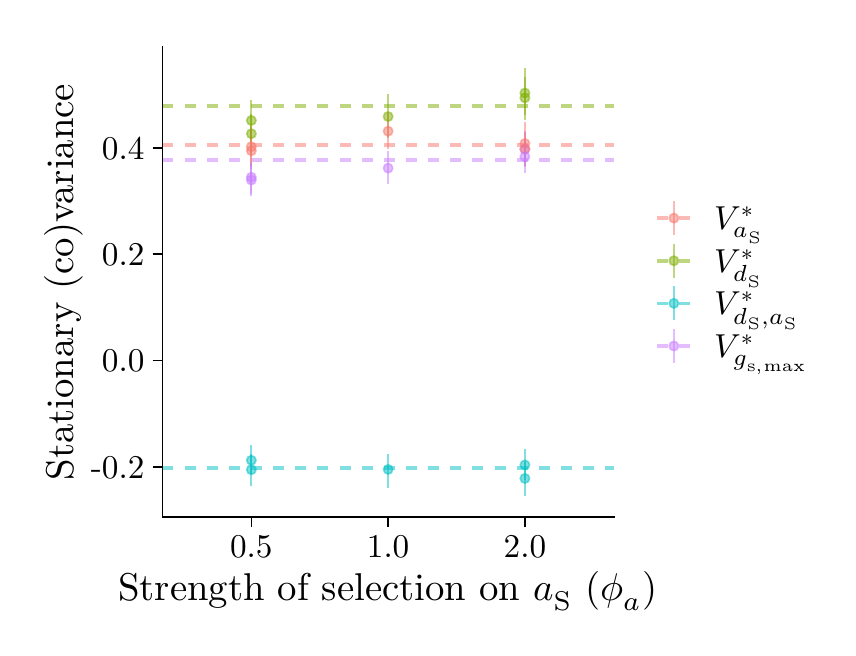
\begin{tikzpicture}[x=1pt,y=1pt]
\definecolor{fillColor}{RGB}{255,255,255}
\path[use as bounding box,fill=fillColor,fill opacity=0.00] (0,0) rectangle (289.08,216.81);
\begin{scope}
\path[clip] ( 48.69, 39.96) rectangle (211.80,209.81);
\definecolor{drawColor}{RGB}{124,174,0}

\path[draw=drawColor,draw opacity=0.50,line width= 1.3pt,dash pattern=on 4pt off 4pt ,line join=round] ( 48.69,188.52) -- (211.80,188.52);
\definecolor{drawColor}{RGB}{248,118,109}

\path[draw=drawColor,draw opacity=0.50,line width= 1.3pt,dash pattern=on 4pt off 4pt ,line join=round] ( 48.69,174.36) -- (211.80,174.36);
\definecolor{drawColor}{RGB}{0,191,196}

\path[draw=drawColor,draw opacity=0.50,line width= 1.3pt,dash pattern=on 4pt off 4pt ,line join=round] ( 48.69, 57.63) -- (211.80, 57.63);
\definecolor{drawColor}{RGB}{199,124,255}

\path[draw=drawColor,draw opacity=0.50,line width= 1.3pt,dash pattern=on 4pt off 4pt ,line join=round] ( 48.69,169.07) -- (211.80,169.07);
\definecolor{drawColor}{RGB}{124,174,0}

\path[draw=drawColor,draw opacity=0.50,line width= 0.7pt,line join=round] (179.67,185.26) -- (179.67,202.09);

\path[draw=drawColor,draw opacity=0.50,line width= 0.7pt,line join=round] (130.25,176.98) -- (130.25,192.77);

\path[draw=drawColor,draw opacity=0.50,line width= 0.7pt,line join=round] (179.67,183.37) -- (179.67,198.99);

\path[draw=drawColor,draw opacity=0.50,line width= 0.7pt,line join=round] ( 80.82,175.92) -- ( 80.82,190.68);
\definecolor{drawColor}{RGB}{248,118,109}

\path[draw=drawColor,draw opacity=0.50,line width= 0.7pt,line join=round] (179.67,167.97) -- (179.67,182.61);

\path[draw=drawColor,draw opacity=0.50,line width= 0.7pt,line join=round] ( 80.82,166.73) -- ( 80.82,181.19);
\definecolor{drawColor}{RGB}{124,174,0}

\path[draw=drawColor,draw opacity=0.50,line width= 0.7pt,line join=round] ( 80.82,171.29) -- ( 80.82,185.68);
\definecolor{drawColor}{RGB}{248,118,109}

\path[draw=drawColor,draw opacity=0.50,line width= 0.7pt,line join=round] ( 80.82,165.78) -- ( 80.82,179.79);

\path[draw=drawColor,draw opacity=0.50,line width= 0.7pt,line join=round] (130.25,173.04) -- (130.25,186.04);
\definecolor{drawColor}{RGB}{199,124,255}

\path[draw=drawColor,draw opacity=0.50,line width= 0.7pt,line join=round] (179.67,166.85) -- (179.67,179.54);
\definecolor{drawColor}{RGB}{248,118,109}

\path[draw=drawColor,draw opacity=0.50,line width= 0.7pt,line join=round] (179.67,166.49) -- (179.67,179.01);
\definecolor{drawColor}{RGB}{0,191,196}

\path[draw=drawColor,draw opacity=0.50,line width= 0.7pt,line join=round] (130.25, 50.47) -- (130.25, 62.93);

\path[draw=drawColor,draw opacity=0.50,line width= 0.7pt,line join=round] (179.67, 47.68) -- (179.67, 59.95);
\definecolor{drawColor}{RGB}{199,124,255}

\path[draw=drawColor,draw opacity=0.50,line width= 0.7pt,line join=round] (179.67,164.38) -- (179.67,176.38);

\path[draw=drawColor,draw opacity=0.50,line width= 0.7pt,line join=round] (130.25,160.49) -- (130.25,172.33);

\path[draw=drawColor,draw opacity=0.50,line width= 0.7pt,line join=round] ( 80.82,155.94) -- ( 80.82,167.70);

\path[draw=drawColor,draw opacity=0.50,line width= 0.7pt,line join=round] ( 80.82,156.73) -- ( 80.82,168.37);
\definecolor{drawColor}{RGB}{0,191,196}

\path[draw=drawColor,draw opacity=0.50,line width= 0.7pt,line join=round] ( 80.82, 51.18) -- ( 80.82, 62.73);

\path[draw=drawColor,draw opacity=0.50,line width= 0.7pt,line join=round] (179.67, 53.19) -- (179.67, 64.72);

\path[draw=drawColor,draw opacity=0.50,line width= 0.7pt,line join=round] ( 80.82, 55.67) -- ( 80.82, 65.88);
\definecolor{drawColor}{RGB}{124,174,0}
\definecolor{fillColor}{RGB}{124,174,0}

\path[draw=drawColor,draw opacity=0.50,line width= 0.6pt,line join=round,line cap=round,fill=fillColor,fill opacity=0.50] (179.67,193.20) circle (  1.69);

\path[draw=drawColor,draw opacity=0.50,line width= 0.6pt,line join=round,line cap=round,fill=fillColor,fill opacity=0.50] (130.25,184.70) circle (  1.69);

\path[draw=drawColor,draw opacity=0.50,line width= 0.6pt,line join=round,line cap=round,fill=fillColor,fill opacity=0.50] (179.67,191.47) circle (  1.69);

\path[draw=drawColor,draw opacity=0.50,line width= 0.6pt,line join=round,line cap=round,fill=fillColor,fill opacity=0.50] ( 80.82,183.28) circle (  1.69);
\definecolor{drawColor}{RGB}{248,118,109}
\definecolor{fillColor}{RGB}{248,118,109}

\path[draw=drawColor,draw opacity=0.50,line width= 0.6pt,line join=round,line cap=round,fill=fillColor,fill opacity=0.50] (179.67,174.97) circle (  1.69);

\path[draw=drawColor,draw opacity=0.50,line width= 0.6pt,line join=round,line cap=round,fill=fillColor,fill opacity=0.50] ( 80.82,173.79) circle (  1.69);
\definecolor{drawColor}{RGB}{124,174,0}
\definecolor{fillColor}{RGB}{124,174,0}

\path[draw=drawColor,draw opacity=0.50,line width= 0.6pt,line join=round,line cap=round,fill=fillColor,fill opacity=0.50] ( 80.82,178.49) circle (  1.69);
\definecolor{drawColor}{RGB}{248,118,109}
\definecolor{fillColor}{RGB}{248,118,109}

\path[draw=drawColor,draw opacity=0.50,line width= 0.6pt,line join=round,line cap=round,fill=fillColor,fill opacity=0.50] ( 80.82,172.34) circle (  1.69);

\path[draw=drawColor,draw opacity=0.50,line width= 0.6pt,line join=round,line cap=round,fill=fillColor,fill opacity=0.50] (130.25,179.41) circle (  1.69);
\definecolor{drawColor}{RGB}{199,124,255}
\definecolor{fillColor}{RGB}{199,124,255}

\path[draw=drawColor,draw opacity=0.50,line width= 0.6pt,line join=round,line cap=round,fill=fillColor,fill opacity=0.50] (179.67,172.84) circle (  1.69);
\definecolor{drawColor}{RGB}{248,118,109}
\definecolor{fillColor}{RGB}{248,118,109}

\path[draw=drawColor,draw opacity=0.50,line width= 0.6pt,line join=round,line cap=round,fill=fillColor,fill opacity=0.50] (179.67,173.01) circle (  1.69);
\definecolor{drawColor}{RGB}{0,191,196}
\definecolor{fillColor}{RGB}{0,191,196}

\path[draw=drawColor,draw opacity=0.50,line width= 0.6pt,line join=round,line cap=round,fill=fillColor,fill opacity=0.50] (130.25, 57.18) circle (  1.69);

\path[draw=drawColor,draw opacity=0.50,line width= 0.6pt,line join=round,line cap=round,fill=fillColor,fill opacity=0.50] (179.67, 53.93) circle (  1.69);
\definecolor{drawColor}{RGB}{199,124,255}
\definecolor{fillColor}{RGB}{199,124,255}

\path[draw=drawColor,draw opacity=0.50,line width= 0.6pt,line join=round,line cap=round,fill=fillColor,fill opacity=0.50] (179.67,170.20) circle (  1.69);

\path[draw=drawColor,draw opacity=0.50,line width= 0.6pt,line join=round,line cap=round,fill=fillColor,fill opacity=0.50] (130.25,166.06) circle (  1.69);

\path[draw=drawColor,draw opacity=0.50,line width= 0.6pt,line join=round,line cap=round,fill=fillColor,fill opacity=0.50] ( 80.82,161.75) circle (  1.69);

\path[draw=drawColor,draw opacity=0.50,line width= 0.6pt,line join=round,line cap=round,fill=fillColor,fill opacity=0.50] ( 80.82,162.77) circle (  1.69);
\definecolor{drawColor}{RGB}{0,191,196}
\definecolor{fillColor}{RGB}{0,191,196}

\path[draw=drawColor,draw opacity=0.50,line width= 0.6pt,line join=round,line cap=round,fill=fillColor,fill opacity=0.50] ( 80.82, 57.08) circle (  1.69);

\path[draw=drawColor,draw opacity=0.50,line width= 0.6pt,line join=round,line cap=round,fill=fillColor,fill opacity=0.50] (179.67, 58.80) circle (  1.69);

\path[draw=drawColor,draw opacity=0.50,line width= 0.6pt,line join=round,line cap=round,fill=fillColor,fill opacity=0.50] ( 80.82, 60.48) circle (  1.69);
\end{scope}
\begin{scope}
\path[clip] (  0.00,  0.00) rectangle (289.08,216.81);
\definecolor{drawColor}{RGB}{0,0,0}

\path[draw=drawColor,line width= 0.6pt,line join=round,line cap=rect] ( 48.69, 39.96) --
	( 48.69,209.81);
\end{scope}
\begin{scope}
\path[clip] (  0.00,  0.00) rectangle (289.08,216.81);
\definecolor{drawColor}{RGB}{0,0,0}

\node[text=drawColor,anchor=base east,inner sep=0pt, outer sep=0pt, scale=  1.20] at ( 42.19, 53.96) {-0.2};

\node[text=drawColor,anchor=base east,inner sep=0pt, outer sep=0pt, scale=  1.20] at ( 42.19, 92.41) {0.0};

\node[text=drawColor,anchor=base east,inner sep=0pt, outer sep=0pt, scale=  1.20] at ( 42.19,130.85) {0.2};

\node[text=drawColor,anchor=base east,inner sep=0pt, outer sep=0pt, scale=  1.20] at ( 42.19,169.30) {0.4};
\end{scope}
\begin{scope}
\path[clip] (  0.00,  0.00) rectangle (289.08,216.81);
\definecolor{drawColor}{RGB}{0,0,0}

\path[draw=drawColor,line width= 0.6pt,line join=round] ( 45.19, 58.10) --
	( 48.69, 58.10);

\path[draw=drawColor,line width= 0.6pt,line join=round] ( 45.19, 96.54) --
	( 48.69, 96.54);

\path[draw=drawColor,line width= 0.6pt,line join=round] ( 45.19,134.99) --
	( 48.69,134.99);

\path[draw=drawColor,line width= 0.6pt,line join=round] ( 45.19,173.43) --
	( 48.69,173.43);
\end{scope}
\begin{scope}
\path[clip] (  0.00,  0.00) rectangle (289.08,216.81);
\definecolor{drawColor}{RGB}{0,0,0}

\path[draw=drawColor,line width= 0.6pt,line join=round,line cap=rect] ( 48.69, 39.96) --
	(211.80, 39.96);
\end{scope}
\begin{scope}
\path[clip] (  0.00,  0.00) rectangle (289.08,216.81);
\definecolor{drawColor}{RGB}{0,0,0}

\path[draw=drawColor,line width= 0.6pt,line join=round] ( 80.82, 36.46) --
	( 80.82, 39.96);

\path[draw=drawColor,line width= 0.6pt,line join=round] (130.25, 36.46) --
	(130.25, 39.96);

\path[draw=drawColor,line width= 0.6pt,line join=round] (179.67, 36.46) --
	(179.67, 39.96);
\end{scope}
\begin{scope}
\path[clip] (  0.00,  0.00) rectangle (289.08,216.81);
\definecolor{drawColor}{RGB}{0,0,0}

\node[text=drawColor,anchor=base,inner sep=0pt, outer sep=0pt, scale=  1.20] at ( 80.82, 25.20) {0.5};

\node[text=drawColor,anchor=base,inner sep=0pt, outer sep=0pt, scale=  1.20] at (130.25, 25.20) {1.0};

\node[text=drawColor,anchor=base,inner sep=0pt, outer sep=0pt, scale=  1.20] at (179.67, 25.20) {2.0};
\end{scope}
\begin{scope}
\path[clip] (  0.00,  0.00) rectangle (289.08,216.81);
\definecolor{drawColor}{RGB}{0,0,0}

\node[text=drawColor,anchor=base,inner sep=0pt, outer sep=0pt, scale=  1.40] at (130.25,  9.72) {Strength of selection on $a_\mathrm{S}$ ($\phi_a$)};
\end{scope}
\begin{scope}
\path[clip] (  0.00,  0.00) rectangle (289.08,216.81);
\definecolor{drawColor}{RGB}{0,0,0}

\node[text=drawColor,rotate= 90.00,anchor=base,inner sep=0pt, outer sep=0pt, scale=  1.40] at ( 16.64,124.89) {Stationary (co)variance};
\end{scope}
\begin{scope}
\path[clip] (  0.00,  0.00) rectangle (289.08,216.81);
\definecolor{drawColor}{RGB}{248,118,109}

\path[draw=drawColor,draw opacity=0.50,line width= 1.3pt,dash pattern=on 4pt off 4pt ,line join=round] (227.34,147.99) -- (239.66,147.99);
\end{scope}
\begin{scope}
\path[clip] (  0.00,  0.00) rectangle (289.08,216.81);
\definecolor{drawColor}{RGB}{248,118,109}

\path[draw=drawColor,draw opacity=0.50,line width= 0.7pt,line join=round] (233.50,141.83) -- (233.50,154.15);
\definecolor{fillColor}{RGB}{248,118,109}

\path[draw=drawColor,draw opacity=0.50,line width= 0.6pt,line join=round,line cap=round,fill=fillColor,fill opacity=0.50] (233.50,147.99) circle (  1.69);
\end{scope}
\begin{scope}
\path[clip] (  0.00,  0.00) rectangle (289.08,216.81);
\definecolor{drawColor}{RGB}{124,174,0}

\path[draw=drawColor,draw opacity=0.50,line width= 1.3pt,dash pattern=on 4pt off 4pt ,line join=round] (227.34,132.59) -- (239.66,132.59);
\end{scope}
\begin{scope}
\path[clip] (  0.00,  0.00) rectangle (289.08,216.81);
\definecolor{drawColor}{RGB}{124,174,0}

\path[draw=drawColor,draw opacity=0.50,line width= 0.7pt,line join=round] (233.50,126.43) -- (233.50,138.75);
\definecolor{fillColor}{RGB}{124,174,0}

\path[draw=drawColor,draw opacity=0.50,line width= 0.6pt,line join=round,line cap=round,fill=fillColor,fill opacity=0.50] (233.50,132.59) circle (  1.69);
\end{scope}
\begin{scope}
\path[clip] (  0.00,  0.00) rectangle (289.08,216.81);
\definecolor{drawColor}{RGB}{0,191,196}

\path[draw=drawColor,draw opacity=0.50,line width= 1.3pt,dash pattern=on 4pt off 4pt ,line join=round] (227.34,117.19) -- (239.66,117.19);
\end{scope}
\begin{scope}
\path[clip] (  0.00,  0.00) rectangle (289.08,216.81);
\definecolor{drawColor}{RGB}{0,191,196}

\path[draw=drawColor,draw opacity=0.50,line width= 0.7pt,line join=round] (233.50,111.03) -- (233.50,123.35);
\definecolor{fillColor}{RGB}{0,191,196}

\path[draw=drawColor,draw opacity=0.50,line width= 0.6pt,line join=round,line cap=round,fill=fillColor,fill opacity=0.50] (233.50,117.19) circle (  1.69);
\end{scope}
\begin{scope}
\path[clip] (  0.00,  0.00) rectangle (289.08,216.81);
\definecolor{drawColor}{RGB}{199,124,255}

\path[draw=drawColor,draw opacity=0.50,line width= 1.3pt,dash pattern=on 4pt off 4pt ,line join=round] (227.34,101.79) -- (239.66,101.79);
\end{scope}
\begin{scope}
\path[clip] (  0.00,  0.00) rectangle (289.08,216.81);
\definecolor{drawColor}{RGB}{199,124,255}

\path[draw=drawColor,draw opacity=0.50,line width= 0.7pt,line join=round] (233.50, 95.63) -- (233.50,107.95);
\definecolor{fillColor}{RGB}{199,124,255}

\path[draw=drawColor,draw opacity=0.50,line width= 0.6pt,line join=round,line cap=round,fill=fillColor,fill opacity=0.50] (233.50,101.79) circle (  1.69);
\end{scope}
\begin{scope}
\path[clip] (  0.00,  0.00) rectangle (289.08,216.81);
\definecolor{drawColor}{RGB}{0,0,0}

\node[text=drawColor,anchor=base west,inner sep=0pt, outer sep=0pt, scale=  1.20] at (248.20,143.85) {$V^*_{a_\mathrm{S}}$};
\end{scope}
\begin{scope}
\path[clip] (  0.00,  0.00) rectangle (289.08,216.81);
\definecolor{drawColor}{RGB}{0,0,0}

\node[text=drawColor,anchor=base west,inner sep=0pt, outer sep=0pt, scale=  1.20] at (248.20,128.45) {$V^*_{d_\mathrm{S}}$};
\end{scope}
\begin{scope}
\path[clip] (  0.00,  0.00) rectangle (289.08,216.81);
\definecolor{drawColor}{RGB}{0,0,0}

\node[text=drawColor,anchor=base west,inner sep=0pt, outer sep=0pt, scale=  1.20] at (248.20,113.05) {$V^*_{d_\mathrm{S},a_\mathrm{S}}$};
\end{scope}
\begin{scope}
\path[clip] (  0.00,  0.00) rectangle (289.08,216.81);
\definecolor{drawColor}{RGB}{0,0,0}

\node[text=drawColor,anchor=base west,inner sep=0pt, outer sep=0pt, scale=  1.20] at (248.20, 97.65) {$V^*_{g_\mathrm{s,max}}$};
\end{scope}
\end{tikzpicture}

\end{figure}

\clearpage

\section*{References}\label{references}
\addcontentsline{toc}{section}{References}

\phantomsection\label{refs}
\begin{CSLReferences}{0}{1}
\bibitem[\citeproctext]{ref-arnold_evolutionary_2023}
\textbf{\textbf{Arnold SJ}}. \textbf{2023}. \emph{Evolutionary
{Quantitative} {Genetics}}. Oxford, United Kingdom: Oxford University
Press.

\bibitem[\citeproctext]{ref-boucher_general_2018}
\textbf{\textbf{Boucher FC}, \textbf{Démery V}, \textbf{Conti E},
\textbf{Harmon LJ}, \textbf{Uyeda J}}. \textbf{2018}.
\href{https://doi.org/10.1093/sysbio/syx075}{A {General} {Model} for
{Estimating} {Macroevolutionary} {Landscapes}}. \emph{Systematic
Biology} \textbf{67}: 304--319.

\bibitem[\citeproctext]{ref-duffield_thermox_2024}
\textbf{\textbf{Duffield S}, \textbf{Donatella K}, \textbf{Melanson D}}.
\textbf{2024}.
\emph{\href{https://github.com/normal-computing/thermox}{Thermox:
{Exact} {OU} processes with {JAX}}}.

\bibitem[\citeproctext]{ref-estes_resolving_2007}
\textbf{\textbf{Estes S}, \textbf{Arnold SJ}}. \textbf{2007}.
\href{https://doi.org/10.1086/510633}{Resolving the {Paradox} of
{Stasis}: {Models} with {Stabilizing} {Selection} {Explain}
{Evolutionary} {Divergence} on {All} {Timescales}}. \emph{The American
Naturalist} \textbf{169}: 227--244.

\bibitem[\citeproctext]{ref-grafen_phylogenetic_1989}
\textbf{\textbf{Grafen A}}. \textbf{1989}.
\href{https://doi.org/10.1098/rstb.1989.0106}{The phylogenetic
regression}. \emph{Philosophical Transactions of the Royal Society of
London. B, Biological Sciences} \textbf{326}: 119--157.

\bibitem[\citeproctext]{ref-hansen_stabilizing_1997}
\textbf{\textbf{Hansen TF}}. \textbf{1997}.
\href{https://doi.org/10.2307/2411186}{Stabilizing selection and the
comparative analysis of adaptation}. \emph{Evolution} \textbf{51}: 1341.

\bibitem[\citeproctext]{ref-hansen_adaptive_2012}
\textbf{\textbf{Hansen TF}}. \textbf{2012}. Adaptive landscapes and the
comparative analysis of adaptation. In: Svensson E, Calsbeek R, eds. The
{Adaptive} {Landscape} in {Evolutionary} {Biology}. Oxford, UK: Oxford
University Press, 205--226.

\bibitem[\citeproctext]{ref-hansen_interpreting_2012}
\textbf{\textbf{Hansen TF}, \textbf{Bartoszek K}}. \textbf{2012}.
\href{https://doi.org/10.1093/sysbio/syr122}{Interpreting the
evolutionary regression: The interplay between observational and
biological errors in phylogenetic comparative studies}. \emph{Systematic
Biology} \textbf{61}: 413--425.

\bibitem[\citeproctext]{ref-hansen_comparative_2008}
\textbf{\textbf{Hansen TF}, \textbf{Pienaar J}, \textbf{Orzack SH}}.
\textbf{2008}. \href{https://doi.org/10.1111/j.1558-5646.2008.00412.x}{A
comparative method for studying adaptation to a randomly evolving
environment}. \emph{Evolution}: 1965--1977.

\bibitem[\citeproctext]{ref-ho_linear-time_2014}
\textbf{\textbf{Ho LST}, \textbf{Ané C}}. \textbf{2014}.
\href{https://doi.org/10.1093/sysbio/syu005}{A linear-time algorithm for
{Gaussian} and non-{Gaussian} trait evolution models}. \emph{Systematic
Biology} \textbf{63}: 397--408.

\bibitem[\citeproctext]{ref-ives_within-species_2007}
\textbf{\textbf{Ives AR}, \textbf{Midford PE}, \textbf{Garland T}}.
\textbf{2007}.
\href{https://doi.org/10.1080/10635150701313830}{Within-{Species}
{Variation} and {Measurement} {Error} in {Phylogenetic} {Comparative}
{Methods}} (T Oakley, Ed.). \emph{Systematic Biology} \textbf{56}:
252--270.

\bibitem[\citeproctext]{ref-kilmer_ordinary_2017}
\textbf{\textbf{Kilmer JT}, \textbf{Rodríguez RL}}. \textbf{2017}.
\href{https://doi.org/10.1111/jeb.12986}{Ordinary least squares
regression is indicated for studies of allometry}. \emph{Journal of
Evolutionary Biology} \textbf{30}: 4--12.

\bibitem[\citeproctext]{ref-lande_natural_1976}
\textbf{\textbf{Lande R}}. \textbf{1976}.
\href{https://doi.org/10.2307/2407703}{Natural {Selection} and {Random}
{Genetic} {Drift} in {Phenotypic} {Evolution}}. \emph{Evolution}
\textbf{30}: 314.

\bibitem[\citeproctext]{ref-lande_quantitative_1979}
\textbf{\textbf{Lande R}}. \textbf{1979}.
\href{https://doi.org/10.2307/2407630}{Quantitative genetic analysis of
multivariate evolution, applied to brain: Body size allometry}.
\emph{Evolution} \textbf{33}: 402--416.

\bibitem[\citeproctext]{ref-lande_genetic_1980}
\textbf{\textbf{Lande R}}. \textbf{1980}.
\href{https://doi.org/10.1093/genetics/94.1.203}{The genetic covariance
between characters maintained by pleiotropic mutations}. \emph{Genetics}
\textbf{94}: 203--215.

\bibitem[\citeproctext]{ref-pennell_model_2015}
\textbf{\textbf{Pennell MW}, \textbf{FitzJohn RG}, \textbf{Cornwell WK},
\textbf{Harmon LJ}}. \textbf{2015}.
\href{https://doi.org/10.1086/682022}{Model adequacy and the
macroevolution of {Angiosperm} functional traits}. \emph{The American
Naturalist} \textbf{186}: E33--E50.

\bibitem[\citeproctext]{ref-pennell_integrative_2013}
\textbf{\textbf{Pennell MW}, \textbf{Harmon LJ}}. \textbf{2013}.
\href{https://doi.org/10.1111/nyas.12157}{An integrative view of
phylogenetic comparative methods: Connections to population genetics,
community ecology, and paleobiology: {Integrative} comparative methods}.
\emph{Annals of the New York Academy of Sciences} \textbf{1289}:
90--105.

\bibitem[\citeproctext]{ref-pennell_macroevolutionary_2024}
\textbf{\textbf{Pennell MW}, \textbf{Jiang D}}. \textbf{2024}.
\href{https://doi.org/10.1093/evolut/qpae015}{The macroevolutionary
adaptive landscape: More than a metaphor?} \emph{Evolution} \textbf{78}:
792--795.

\bibitem[\citeproctext]{ref-rolland_conceptual_2023}
\textbf{\textbf{Rolland J}, \textbf{Henao-Diaz LF}, \textbf{Doebeli M},
\textbf{Germain R}, \textbf{Harmon LJ}, \textbf{Knowles LL},
\textbf{Liow LH}, \textbf{Mank JE}, \textbf{Machac A}, \textbf{Otto SP},
\emph{et al.}} \textbf{2023}.
\href{https://doi.org/10.1038/s41559-023-02116-7}{Conceptual and
empirical bridges between micro- and macroevolution}. \emph{Nature
Ecology \& Evolution} \textbf{7}: 1181--1193.

\bibitem[\citeproctext]{ref-sack_trait_2020}
\textbf{\textbf{Sack L}, \textbf{Buckley TN}}. \textbf{2020}.
\href{https://doi.org/10.1093/icb/icz152}{Trait {Multi}-{Functionality}
in {Plant} {Stress} {Response}}. \emph{Integrative and Comparative
Biology} \textbf{60}: 98--112.

\bibitem[\citeproctext]{ref-uyeda_novel_2014}
\textbf{\textbf{Uyeda JC}, \textbf{Harmon LJ}}. \textbf{2014}. A novel
{Bayesian} method for inferring and interpreting the dynamics of
adaptive landscapes from phylogenetic comparative data. \emph{Systematic
Biology} \textbf{64}: 902--918.

\bibitem[\citeproctext]{ref-warton_bivariate_2006}
\textbf{\textbf{Warton DI}, \textbf{Wright IJ}, \textbf{Falster DS},
\textbf{Westoby M}}. \textbf{2006}.
\href{https://doi.org/10.1017/S1464793106007007}{Bivariate line-fitting
methods for allometry}. \emph{Biological Reviews} \textbf{81}: 259.

\end{CSLReferences}



\end{document}
